% !TeX root = ./eLife_draft.tex
\documentclass[9pt,lineno]{elife}
\usepackage[version=4]{mhchem}
\usepackage{siunitx}
\title{Fundamental limits on the rate of bacterial cell division}
\author[$\dagger$, 1]{Nathan M. Belliveau}
\author[$\dagger$, 2]{Griffin Chure}
\author[3]{Christina L. Hueschen}
\author[4]{Hernan G. Garcia}
\author[5]{Jane Kondev}
\author[6]{Daniel S. Fisher}
\author[1, 7, *]{Julie A. Theriot}
\author[8, 9, *]{Rob Phillips}
\affil[1]{Department of Biology, University of Washington, Seattle, WA, USA}
\affil[2]{Department of Applied Physics, California Institute of Technology, Pasadena, CA, USA}
\affil[3]{Department of Chemical Engineering, Stanford University, Stanford, CA, USA}
\affil[4]{Department of Molecular Cell Biology and Department of Physics, University of California Berkeley, Berkeley, CA, USA}
\affil[5]{Department of Physics, Brandeis University, Waltham, MA, USA}
\affil[6]{Department of Applied Physics, Stanford University, Stanford, CA, USA}
\affil[7]{Allen Institute for Cell Science, Seattle, WA, USA}
\affil[8]{Division of Biology and Biological Engineering, California Institute of Technology, Pasadena, CA, USA}
\affil[9]{Department of Physics, California Institute of Technology, Pasadena, CA, USA}
\affil[*]{Co-corresponding authors. Address correspondence to phillips@pboc.caltech.edu and jtheriot@uw.edu}
\contrib[$\dagger$]{These authors contributed equally to this work}

\begin{document}
\maketitle
\begin{abstract}
Recent years have seen a deluge of experiments dissecting the relationship
between bacterial growth rate, cell size, and protein content, quantifying
the abundance of proteins across growth conditions with unprecedented
resolution. However, we still lack a rigorous understanding of what sets the
scale of these quantities and when protein abundances should (or should not)
depend on growth rate. Here, we seek to quantitatively understand this
relationship across a collection of \textit{Escherichia coli} proteomic data
sets covering $\approx$ 4000 proteins and 36 growth rates. We estimate
the basic requirements for steady-state growth by considering key processes
in nutrient transport, energy generation, cell envelope biogenesis, and the
central dogma. From these estimates, ribosome biogenesis emerges as a primary
determinant of growth rate. We expand on this assessment by exploring a model of proteomic
regulation as a function of the nutrient supply, revealing a mechanism that
ties cell size and growth rate to ribosomal content.

\end{abstract}

% !TeX root = ./eLife_draft.tex

\section{Introduction}
The observed range of bacterial growth rates is enormously diverse. In natural
environments, some microbial organisms may double only once per year
\citep{mikucki2009} while in comfortable laboratory conditions, growth can be
rapid with several divisions per hour \citep{schaechter1958}. This six
order-of-magnitude difference in time scales of growth encompasses different
microbial species and lifestyles, yet even for a single species such as
\textit{Escherichia coli}, the growth rate can be modulated over a
large scale by tuning the type and amount of nutrients in the growth medium
\citep{liu2005a}. This remarkable plasticity in growth rate illustrates the
intimate relationship between environmental conditions and the rates at which
cells convert nutrients into new cellular material -- a relationship that has
remained a major topic of inquiry in bacterial physiology for over a century
\citep{jun2018}.

A key discovery in bacterial physiology of the past 70 years was the
identification of bacterial "growth laws" \citep{schaechter1958}; empirical
relationships that relate the bacterial growth rate to the protein and RNA
composition of the intracellular milieu in a number of different species.
Over the past decade, a flurry of work \citep{molenaar2009, scott2010,
klumpp2014, basan2015, dai2016, erickson2017} has examined these growth laws
at a quantitative level, developing a series of phenomenological models from
which the growth laws naturally emerge. In parallel, a "molecular revolution"
in biology has yielded an increasingly refined molecular census of the cell,
particularly for bacteria such as the microbial workhorse \textit{E. coli}
\citep{schmidt2016, davidi2016a}. In light of the now expansive trove of
quantitative biological data, we can revisit several of the evergreen
questions about bacterial growth and physiology that were originally raised
by microbiologists in the middle of the 20th century. Specifically, what
biological processes are the primary determinants for how quickly bacterial
cells can grow and reproduce? Why do cells modulate the absolute numbers and
relative ratios of their molecular constituents as a function of changes in
growth rate or nutrient availability?

In this work, we begin by considering these two questions from two distinct
angles. First, as a result of an array of high-quality proteome-wide
measurements of \textit{E. coli} under diverse growth conditions, we have
generated a census that allows us to explore how the number of key molecular
players change as a function of growth rate. Here, we have assembled a singular
data set of protein copy numbers using measurements collected over the past
decade via mass spectrometry \citep{schmidt2016, peebo2015, valgepea2013} or
ribosomal profiling \citep{li2014} of the composition of the \textit{E. coli}
proteome across a gamut of growth rates. Due to notable changes in cell size and
cellular composition as a function of growth rate \citep{bremer2008,
taheriaraghi2015}, as well as differences in normalization and standardization
schemes used in each experimental work, substantial care was taken to ensure
consistency on a per cellular basis (see the Appendix for a detailed analysis
and additional discussion). To our knowledge, this compiled and curated dataset
represents the most comprehensive view to date of the \textit{E. coli} proteome,
covering $\approx$ 4000 proteins and 36 unique growth rates, with the observed
abundance of any given protein being directly comparable between data sets and
across growth rates. This allows us to interrogate  the \textit{E. coli}
specific physiology underlying the observed abundances while  minimizing the
effects of experimental noise, as  $\approx$ 75\% of the  proteins are observed
in at least two separate datasets.

Second, by compiling molecular turnover rate measurements for many of the
fundamental processes associated with bacterial growth, we make quantitative
estimates of a handful of key cellular processes (schematized in
\FIG{categories}) to determine whether our current understanding of the
kinetics of these processes are sufficient to explain the magnitude of the
observed protein copy numbers across conditions (see \BOX{estimate_rules}
describing the philosophy behind this approach). The census, combined with
these estimates, provide a window into the question of whether the rates of
central processes such as energy generation or DNA synthesis vary
systematically as a function of cell growth rate by altering protein copy
number.

Throughout our estimates, we consider an archetypal growth rate of $\approx$
0.5 hr$^{-1}$ corresponding to a doubling time of $\approx$ 5000 seconds, as
the data sets examined here heavily sample this growth regime. While we
formulate point estimates for the protein abundances at this division time,
we also consider how these values will vary at other growth rates due to
changes in cell size, surface area, and chromosome copy number
\citep{taheriaraghi2015, harris2018}. For the majority of the processes
considered, we find that the protein copy numbers appear tuned for the task
of cell doubling across a continuum of growth rates. Thus, our understanding
of the kinetics of various biological processes is sufficient to
quantitatively explain the observed abundances of these proteins.

% From these estimates, it emerges that translation, particularly the synthesis of
% ribosomal proteins, is a plausible candidate that limits the rate of cellular
% growth in \textit{E. coli}.

From these estimates, it emerges that translation,  particularly the synthesis of ribosomal proteins is a
plausible candidate that limits the rate of cellular growth in \textit{E. coli}.
We reach this conclusion by considering that ribosome synthesis is 1) a rate
limiting step for the \textit{fastest} bacterial division, and  2) the main
determinant of bacterial growth rate across  nutrient conditions associated with
moderate to fast growth rates. In addition, a strict dependence between the
maximal growth rate and ribosomal mass fraction coincides with the regime where
the growth laws appear most valid \citep{amir2017, scott2010}. This enables us
to suggest that the long-observed correlation between growth rate and cell size
\citep{schaechter1958, si2017} can be simply attributed to the increased
absolute number of ribosomes per cell under conditions supporting extremely
rapid growth. To better understand how the observed alterations in absolute
protein abundances, and in particular, changes in ribosome copy number,
influence growth rate across different nutrient conditions we consider a minimal
model of cellular growth. Our conclusions from these analyses provide important
insight into how \textit{E. coli} regulates growth across conditions of
differing nutrient availability and identifies fundamental constraints in
bacterial growth more broadly.






\begin{figure}
    \centering{
    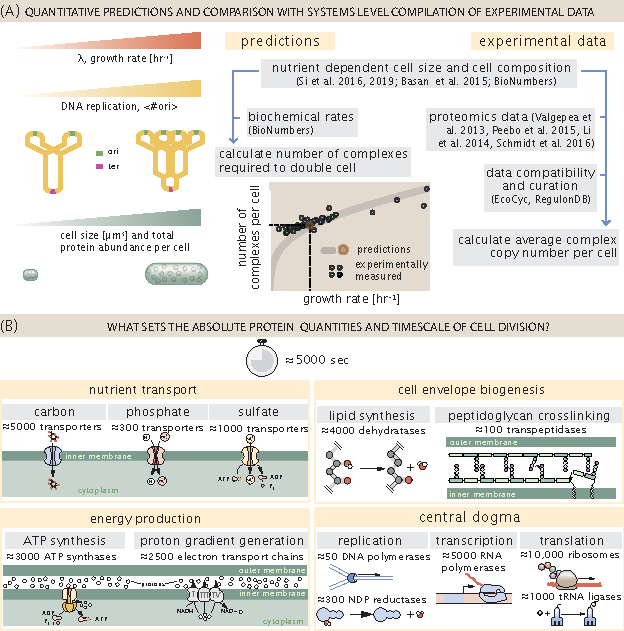
\includegraphics{main_figs/fig1_schematic_categories_grouped.pdf}
    \caption{\textbf{Transport and synthesis processes necessary for cell division.}
            We consider an array of processes necessary for a cell to double its
            molecular components, broadly grouped into four classes. These
            categories are (A) nutrient transport across the cell membrane, (B) cell envelope
            biogenesis, (C) energy production (namely, ATP synthesis), and (D) processes associated with the central dogma.
            Numbers shown are the approximate number of complexes of each type
            observed at a growth rate of 0.5 hr$^{-1}$, or a cell doubling time
            of $\approx$ 5000 s.}
    \label{fig:categories}
    }
\end{figure}

\section{Uptake of Nutrients}
In order to build new cellular mass, the molecular and elemental building blocks
must be scavenged from the environment in different forms. Carbon, for example,
is acquired via the transport of carbohydrates and sugar alcohols with some
carbon sources receiving preferential treatment in their consumption
\citep{monod1947}. Phosphorus, sulfur, and nitrogen, on the other hand, are
harvested primarily in the forms of inorganic salts, namely phosphate, sulfate,
and ammonia \citep{jun2018, assentoft2016, stasi2019, antonenko1997,
rosenberg1977, willsky1973}. All of these compounds have different
permeabilities across the cell membrane \cite{phillips2018} and  most require some energetic
investment either via ATP hydrolysis or through the proton electrochemical
gradient to bring the material across the hydrophobic cell membrane. Given the
diversity of biological transport mechanisms and the vast number of inputs
needed to build a cell, we begin by considering transport of some of the most
important cellular ingredients: carbon, nitrogen, oxygen, hydrogen, phosphorus,
and sulfur.

The elemental composition of \textit{E. coli} has received much quantitative
attention over the past half century \citep{neidhardt1991, taymaz-nikerel2010,
heldal1985, bauer1976}, providing us with a starting point for estimating the
copy numbers of various transporters. While there is some variability in the
exact elemental percentages (with different uncertainties), we can estimate that
the dry mass of a typical \textit{E. coli} cell is $\approx$ 45\% carbon (BNID:
100649, \cite{milo2010}), $\approx$ 15\% nitrogen (BNID: 106666,
\cite{milo2010}), $\approx$ 3\% phosphorus (BNID: 100653, \cite{milo2010}), and
1\% sulfur (BNID: 100655, \cite{milo2010}). In the coming paragraphs, we will
engage in a dialogue between back-of-the-envelope estimates for the numbers of
transporters needed to facilitate these chemical stoichiometries and the
experimental proteomic measurements of the biological reality. Such an approach
provides the opportunity to test if our biological knowledge is sufficient to
understand the scale at which these complexes are produced. Specifically, we
will make these estimates considering a modest doubling time of 5000 s, a growth
rate of $\approx$ 0.5 hr$^{-1}$, the range in which the majority of the
experimental measurements reside.

\subsection{Nitrogen Transport}
Before we begin our back-of-the-envelope estimations, we must address which
elemental sources must require proteinaceous transport, meaning that the cell
cannot acquire appreciable amounts simply via diffusion across the membrane.
The permeability of the lipid membrane to a large number of solutes has been
extensively characterized over the past century. Large, polar
molecular species (such as various sugar molecules, sulfate, and phosphate) have
low permeabilities  while small, non-polar compounds (such as oxygen, carbon
dioxide, and ammonia) can readily diffuse across the
membrane. Ammonia, a primary source of nitrogen in typical laboratory
conditions, has a permeability on par with water ($\approx 10^5$ nm/s,
BNID:110824 \cite{milo2010}). In particularly nitrogen-poor
conditions, \textit{E. coli} expresses a transporter (AmtB) which appears to aid in
nitrogen assimilation, though the mechanism and kinetic details of transport
are still a matter of debate \citep{heeswijk2013a, khademi2004}. Beyond ammonia,
another plentiful source of nitrogen come in the form of glutamate, which has it's
own complex metabolism and scavenging pathways. However, nitrogen is plentiful
in the growth conditions examined in this work, permitting us to neglect
nitrogen transport as a potential rate limiting process in cell division in
typical experimental conditions. We direct the reader to the supplemental
information for a more in-depth discussion of permeabilities and a series of
calculations revealing that active nitrogen transport can be neglected for the
purposes of this article.

\subsection{Carbon Transport}
We begin our estimations with the most abundant element in \textit{E. coli}
by mass, carbon. Using $\approx$ 0.3 pg as the typical \textit{E. coli} dry
mass (BNID: 103904, \cite{milo2010}), we estimate that $\approx 10^{10}$
carbon atoms must be brought into the cell in order to double all of the
carbon-containing molecules (\FIG{carbon_tport}(A, top)). Typical laboratory
growth conditions, such as those explored in the aforementioned proteomic
data sets, provide carbon as a single class of sugar such as glucose,
galactose, or xylose to name a few. \textit{E. coli} has evolved myriad
mechanisms by which these sugars can be transported across the cell membrane.
One such mechanism of transport is via the PTS system which is a highly
modular system capable of transporting a diverse range of sugars
\citep{escalante2012}. The glucose-specific component of this system
transports $\approx$ 200 glucose molecules per second per transporter (BNID:
114686, \cite{milo2010}). Making the assumption that this is a typical sugar
transport rate, coupled with the need to transport 10$^{10}$ carbon atoms, we
arrive at the conclusion that on the order of 1,000 transporters must be
expressed in order to bring in enough carbon atoms to divide in 5000 s,
diagrammed in the top panel of \FIG{carbon_tport}(A). This estimate, along
with the observed average number of the PTS system carbohydrate transporters present in the
proteomic data sets \citep{schmidt2016, peebo2015,valgepea2013,li2014}, is
shown in \FIG{carbon_tport}(A). While we estimate 1500 transporters are
needed with a 5000 s division time, we can abstract this calculation to consider
any particular growth rate given knowledge of the cell density and volume as a
function of growth rate and direct the reader to the SI for more information. As
revealed in \FIG{carbon_tport}(A), experimental measurements exceed the estimate
by several fold, illustrating that transport of carbon into the cell is not
rate limiting for cell division. Abstracting this point estimate at 5000 s to a
continuum of growth rates (grey line in \FIG{carbon_tport}(A)) reveals an excess
of transporters at other growth rates, though in rapid growth regimes, the
abundance is below our simple estimate.
\begin{figure}
    \begin{fullwidth}
    \centering{
    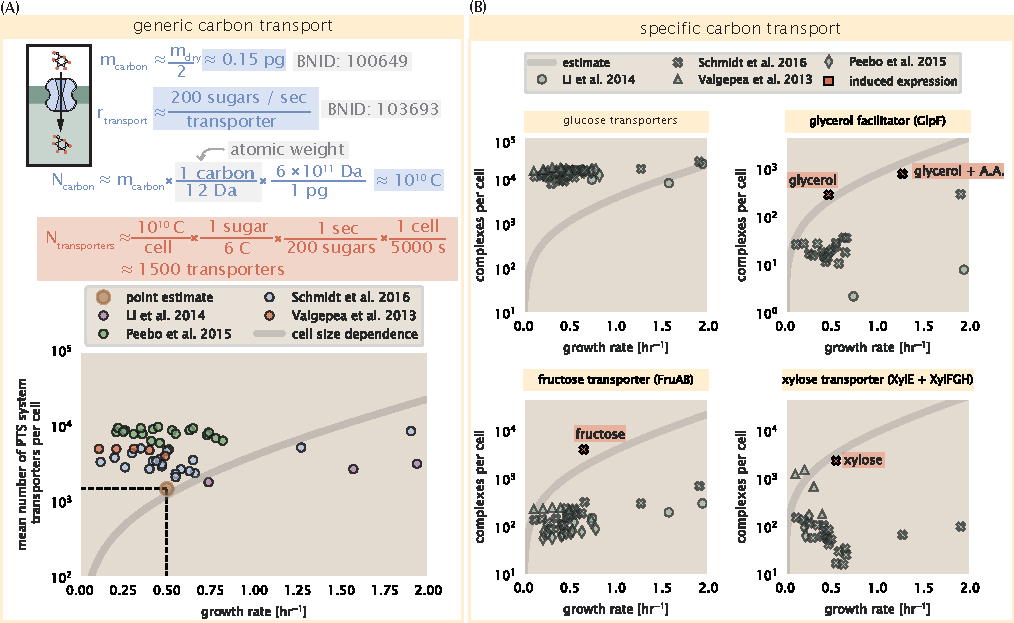
\includegraphics{main_figs/fig2_carbon_transport.pdf}
    \caption{\textbf{The abundance of carbon transport systems across growth
    rates.} (A) A simple estimate for the minimum number of generic carbohydrate
    transport systems (top) assumes $\approx 10^{10}$ C are needed to complete
    division, each transported sugar contains $\approx 6$ C, and each
    transporter conducts sugar molecules at a rate of $\approx 200$ per second.
    Bottom plot shows the estimated number of transporters needed at a growth
    rate of $\approx 0.5 $ per hr (light-brown point and dashed lines).  Colored
    points correspond to the mean number of PTS system sugar transporters
    (complexes annotated with the Gene Ontology term GO:0009401) for
    different growth conditions across different published datasets. (B) The
    abundance of various specific carbon transport systems plotted as a function
    of the population growth rate. The rates of substrate transport to compute
    the continuum growth rate estimate (grey line) were 200 glucose$\cdot$
    s$^{-1}$ (BNID: 103693, \cite{milo2010}),  2000 glycerol$\cdot$s$^{-1}$
    \citep{lu2003}, 200 fructose$\cdot$
    s$^{-1}$ (assumed to be similar to PtsI, BNID: 103693, \cite{milo2010}), and 50 xylose$\cdot$s$^{-1}$
    (assumed to be comparable to LacY, BNID:103159, \cite{milo2010}).
    Red points and highlighted text indicate conditions in
    which the
    only source of carbon in the growth medium induces expression of the
    transport system. Grey line in (A) and (B) represents the estimated number of transporters per cell at a continuum
    of growth rates.}
    \label{fig:carbon_tport}
    }
    \end{fullwidth}
\end{figure}

The estimate presented in \FIG{carbon_tport}(A) neglects any specifics of the
regulation of the carbon transport system and presents a  view of how
many carbohydrate transporters are present on average. Using the diverse array
of growth conditions explored in the proteomic data sets, we can explore how
individual carbon transport systems depend on the population growth rate. In
\FIG{carbon_tport}(B), we show the total number of carbohydrate transporters
specific to different carbon sources. A striking observation, shown in the
top-left plot of \FIG{carbon_tport}(B), is the constancy in the expression of the
glucose-specific transport systems. Additionally, we note that the total number
of glucose-specific transporters is tightly distributed at $\approx 10^4$ per cell,
the approximate number of transporters needed to sustain rapid growth of several
divisions per hour. This
illustrates that \textit{E. coli} maintains a substantial number of complexes
present for transporting glucose regardless of growth rate, which is known to be the preferential carbon
source \citep{monod1947, liu2005a, aidelberg2014}.

It is now understood that a large number of metabolic operons are regulated
with dual-input logic gates that are only expressed when glucose
concentrations are low (mediated by cyclic-AMP receptor protein CRP) and the
concentration of other carbon sources are elevated \citep{gama-castro2016, zhang2014a}. A
famed example of such dual-input regulatory logic is in the regulation of the
\textit{lac} operon which is only natively activated in the absence of glucose and the
presence of allolactose, an intermediate in lactose metabolism \citep{jacob1961}, though
we now know of many other such examples \citep{ireland2020, gama-castro2016,
belliveau2018}. This illustrates that once glucose is depleted from the
environment, cells have a means to dramatically increase the abundance of the
specific transporter needed to digest the next sugar that is present. Several
examples of induced expression of specific carbon-source transporters are
shown in \FIG{carbon_tport}(B). Points colored in red (labeled by red
text-boxes) correspond to growth conditions in which the specific carbon source
(glycerol, xylose, or fructose) is present. These plots show that, in the
absence of the particular carbon source, expression of the transporters is
maintained on the order of $\sim 10^2$ per cell. However, when the transport
substrate is present, expression is induced and the
transporters become highly-expressed. The grey lines in \FIG{carbon_tport}(B)
show the estimated number of transporters needed at each growth rate to satisfy
the cellular carbon requirement. It is notable that  in all cases, the magnitude
of induced expression (shown in red) falls close to the estimate, illustrating
the ability of the cell to tune expression in response to changing environments. Together, this generic estimation and the specific
examples of induced expression suggest that transport of carbon across the cell
membrane, while critical for growth, is not the rate-limiting step of cell division.

\subsection{Phosphorus and Sulfur Transport}
We now turn our attention towards other essential elements, namely phosphorus and
sulfur. Phosphorus is critical to the cellular energy economy in the form of
high-energy phosphodiester bonds making up DNA, RNA, and the NTP energy pool as
well as playing a critical role in the post-translational modification of
proteins and defining the polar-heads of lipids. In total, phosphorus
makes up $\approx$3\% of the cellular dry mass which in typical experimental conditions is in the form of inorganic phosphate. The cell membrane
has remarkably low permeability to this highly-charged and critical molecule,
therefore requiring the expression of active transport systems. In \textit{E. coli}, the proton
electrochemical gradient across the inner membrane is leveraged to transport
inorganic phosphate into the cell \citep{rosenberg1977}.
Proton-solute symporters are widespread in \textit{E. coli} \citep{ramos1977,
booth1979} and can have rapid transport rates of 50 to 100 molecules per second for
sugars and other solutes (BNID: 103159; 111777, \cite{milo2010}). As a more
extreme example, the proton transporters in the F$_1$-F$_0$ ATP synthase, which
use the proton electrochemical gradient for rotational motion, can shuttle
protons across the membrane at a rate of $\approx$ 1000 per second (BNID:
104890; 103390, \citep{milo2010}). In \textit{E.
coli} the PitA phosphate transport system has been shown to be very tightly coupled
with the proton electrochemical gradient with a 1:1 proton:phosphate
stoichiometric ratio \citep{harris2001, feist2007}. Taking the geometric mean of
the aforementioned estimates gives a plausible rate of phosphate transport on
the order of 300  per second. Illustrated in
\FIG{phospho_sulfo_tport}(A), we can estimate that $\approx$ 150
phosphate transporters are necessary to maintain an $\approx$ 3\% dry mass with
a 5000 s division time. This estimate is consistent with observation when we examine the
observed copy numbers of PitA in proteomic data sets (plot in
\FIG{phospho_sulfo_tport}(A)). While our estimate is very much in line with the
observed numbers, we emphasize that this is likely a slight overestimate of the
number of transporters needed as there are other phosphorous scavenging systems,
such as the ATP-dependent phosphate transporter Pst system which we have neglected.

Satisfied that there are a sufficient number of phosphate transporters
present in the cell, we now turn to sulfur transport as another potentially rate
limiting process. Similar to phosphate, sulfate is  highly-charged
and not particularly membrane permeable, requiring active
transport. While there exists a H+/sulfate symporter in \textit{E.
coli}, it is in relatively low abundance and is not well characterized
\citep{zhang2014}. Sulfate is predominantly acquired via the ATP-dependent ABC
transporter CysUWA system which also plays an important role in selenium
transport \citep{sekowska2000, sirko1995}. While specific kinetic details of
this transport system are not readily available, generic ATP transport
systems in prokaryotes transport on the order of 1 to 10 molecules per second
(BNID: 109035, \cite{milo2010}). Combining this generic
transport rate, measurement of sulfur comprising 1\% of dry mass, and a 5000
second division time yields an estimate of $\approx$ 1000 CysUWA
complexes per cell (\FIG{phospho_sulfo_tport}(B)). Once again, this estimate
is in notable agreement with proteomic data sets, suggesting that there are
sufficient transporters present to acquire the necessary sulfur. In a similar
spirit of our estimate of phosphorus transport, we emphasize that this is
likely an overestimate of the number of necessary transporters as we have
neglected other sulfur scavenging systems that are in lower abundance.


\begin{figure*}
    \begin{fullwidth}
    \centering{
        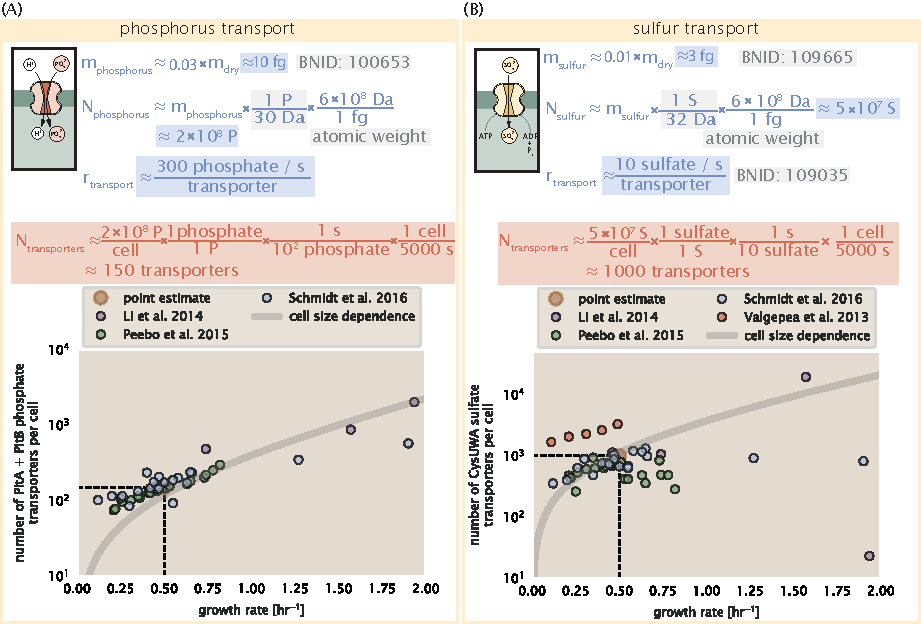
\includegraphics{main_figs/fig3_phospho_sulfo_transport.pdf}
        \caption{\textbf{Estimates and measurements of phosphate and sulfate
        transport systems as a function of growth rate.} (A) Estimate for the
        number of PitA phosphate transport systems needed to maintain a 3\%
        phosphorus \textit{E. coli} dry mass. Points in plot correspond to
        the the total number of PitA transporters per cell. (B) Estimate of
        the number of CysUWA complexes necessary to maintain a 1\% sulfur
        \textit{E. coli} dry mass. Points in plot correspond to average
        number of CysUWA transporter complexes that can be formed given the
        transporter stoichiometry [CysA]$_2$[CysU][CysW][Sbp/CysP]. Grey line
        in (A) and (B) represents the estimated number of transporters per
        cell at a continuum of growth rates.}
        \label{fig:phospho_sulfo_tport}
    }
    \end{fullwidth}
\end{figure*}


\subsection{Limits on Transporter Expression}
So which, if any, of these processes may be rate limiting for growth? As
suggested by \FIG{carbon_tport} (B), induced expression can lead to an
order-of-magnitude (or more) increase in the amount of transporters needed to
facilitate transport. Thus, if acquisition of nutrients was the limiting state
in cell division, could expression simply be increased to accommodate faster
growth? A way to approach this question is to compute the amount of space in the
bacterial membrane that could be occupied by nutrient transporters. Considering a rule-of-thumb for the surface area of
\textit{E. coli} of about 6 \textmu m$^2$ (BNID: 101792, \cite{milo2010}), we expect
an areal density for 1000 transporters to be approximately 200
transporters/ \textmu m$^2$. For a typical transporter occupying about 50
nm$^2$/dimer, this amounts to about only 1 percent of the total inner membrane
\citep{szenk2017}. In addition, bacterial cell membranes typically have
densities of 10$^5$ proteins/$\mu m^2$ \citep{phillips2018}, implying that the
cell could accommodate more transporters of a variety of species if it were rate
limiting. As we will see in the next section, however, occupancy of the membrane can
impose other limits on the rate of energy production.

% \section{Energy Production}
Cells consume and generate energy predominantly in the form of nucleoside
triphosphates (NTPs) in order to grow. The high-energy phosophodiester bonds of
(primarily) ATP power a variety of cellular processes that drive biological
systems away from thermodynamic equilibrium. We now turn to the synthesis of ATP
as a potential process that may limit growth, which also requires us to consider
the maintenance of the electrochemical proton gradient which powers it.

\subsection{ATP Synthesis}
Hydrolysis of the terminal phosphodiester bond of ATP into ADP (or
alternatively GTP and GDP) and an inorganic phosphate provides the
thermodynamic driving force in a wide array of biochemical reactions. One
such reaction is the formation of peptide bonds during translation, which
requires $\approx$ 2 ATPs for the charging of an amino acid to the tRNA and
$\approx$ 2 GTPs for the formation of each peptide bond. Assuming the ATP
costs associated with error correction and post-translational modifications
of proteins are negligible, we can make the approximation that each peptide
bond has a net cost of $\approx$ 4 ATP (BNID: 101442).
Formation of GTP from ATP is achieved via the action of nucleoside
diphosphate kinase, which catalyzes this reaction without an energy
investment \citep{lascu2000} and therefore consider all NTP requirements of
the cell to be functionally equivalent to being exclusively ATP. In total,
the energetic costs of peptide bond formation consume $\approx$ 80\% of the
cells ATP budget [BNID: 107782; 106158; 101637; 111918,
\cite{lynch2015,stouthamer1973}]. The pool of ATP is produced by the
F$_1$-F$_0$ ATP synthase -- a membrane-bound rotary motor which under ideal
conditions can yield $\approx$ 300 ATP per second [BNID: 114701;
\cite{weber2003}].

To estimate the total number of ATP equivalents consumed during a cell cycle, we
will make the approximation that there are $\approx 3\times10^6$ proteins per
cell with an average protein length of $\approx$ 300 peptide bonds (BNID:
115702; 108986; 104877). Taking these values together, coupled with an estimate
of $\approx$ 4 ATP equivalents per peptide bond, we find that the typical
\textit{E. coli} cell consumes $\sim 5 \times 10^9$ ATP per cell cycle on
protein synthesis alone. Assuming that each ATP synthases operates at its
maximal speed (300 ATP per second per synthase), $\approx$ 3000 ATP synthases
are needed to keep up with the energy demands of the cell. This estimate
is comparable with the experimental observations,  shown in
\FIG{energy_production} (A). We note that this estimate assumes all ATP is
synthesized via ATP synthase and neglects synthesis via fermentative metabolism.
This simplification may explain why at the fastest growth rates ($\approx$ 2
hr$^{-1}$), our continuum estimate predicts more synthase than is experimentally
observed (gray line in \FIG{energy_production}). At rapid growth rates,
\textit{E. coli} enters a type of overflow metabolism where fermentative
metabolism becomes pronounced \citep{szenk2017}.

\subsection{Generating the Proton Electrochemical Gradient}
In order to produce ATP, the F$_1$-F$_0$ ATP synthase itself must consume
energy. Rather than burning through its own product (and violating
thermodynamics), this intricate macromolecular machine has evolved to exploit
the electrochemical potential established across the inner membrane through
cellular respiration. This electrochemical gradient is manifest by the pumping
of protons into the intermembrane space via the electron transport chains as
they reduce NADH. In \textit{E. coli}, this potential difference is $\approx
-$200 mV (BNID: 102120). A simple estimate of the inner membrane as a capacitor
with a working voltage of -200 mV reveals that $\approx 2\times 10^4$ protons
must be present in the intermembrane space. However, each rotation of an ATP
synthase shuttles $\approx$ 4 protons into the cytosol (BNID: 103390). With a few thousand ATP
synthases producing ATP at their maximal rate, the potential difference would be
rapidly abolished in a few milliseconds if it were not being actively
maintained.

The electrochemistry of the electron transport complexes of \textit{E. coli}
have been the subject of intense biochemical and biophysical study
\citep{ingledew1984, khademian2017,cox1970,henkel2014}. A recent work
\citep{szenk2017} examined the respiratory capacity of the \textit{E. coli}
electron transport complexes using structural and biochemical data, revealing
that each electron transport chain rapidly pumps protons into the
intermembrane space at a rate of $\approx$ 1500 protons per second (BIND:
114704; 114687). Using our estimate of the number of ATP synthases required
per cell [\FIG{energy_production}(A)], coupled with these recent
measurements, we estimate that $\approx 3000$ electron transport complexes
would be necessary to facilitate the $\sim 5 \times 10^6$ protons per second
diet of the cellular ATP synthases. This estimate is in agreement with the
number of complexes identified in the proteomic datasets [plot in
\FIG{energy_production}(B)]. This suggests that every ATP synthase must be
accompanied by $\approx$ 1 functional electron transport chain.

\begin{figure}
    \begin{fullwidth}
        \centering{
            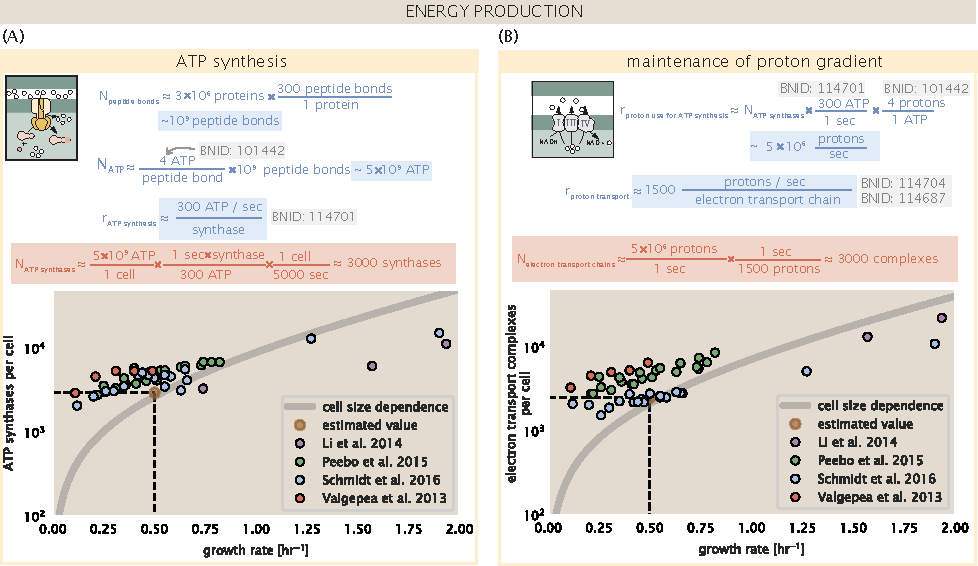
\includegraphics{main_figs/fig4_energy_production.pdf}
            \caption{\textbf{The abundance of F$_1$-F$_0$ ATP synthases and
            electron transport chain complexes as a function of growth
            rate.} (A) Estimate of the number of F$_1$-F$_0$ ATP synthase
            complexes needed to accommodate peptide bond formation and other NTP
            dependent processes. Points in plot correspond to the
            mean number of complete F$_1$-F$_0$ ATP synthase complexes that
            can be formed given proteomic measurements and the subunit
            stoichiometry
            [AtpE]$_{10}$[AtpF]$_2$[AtpB][AtpC][AtpH][AtpA]$_{3}$[AtpG][AtpD]$_3$.
            (B) Estimate of the number of electron transport chain complexes
            needed to maintain a membrane potential of $-$200 mV given
            estimate of number of F$_1$-F$_0$ ATP synthases from (A). Points
            in plot correspond to the average number of complexes identified
            as being involved in aerobic respiration by the Gene Ontology
            identifier GO:0019646 that could be formed given proteomic
            observations. These complexes include cytochromes \textit{bd1}
            ([CydA][CydB][CydX][CydH]), \textit{bdII} ([AppC][AppB]),
            \textit{bo$_3$},([CyoD][CyoA][CyoB][CyoC]) and NADH:quinone
            oxioreducase I
            ([NuoA][NuoH][NuoJ][NuoK][NuoL][NuoM][NuoN][NuoB][NuoC][NuoE][NuoF][NuoG][NuoI])
            and II ([Ndh]). Grey lines in both (A) and (B) correspond to the
            estimate procedure described, but applied to a continuum of growth
            rates. We direct the reader to the Supporting Information for a more
            thorough description of this approach.}
        \label{fig:energy_production}
        }
    \end{fullwidth}
\end{figure}


\subsubsection{Limits on Biosynthesis in a Crowded Membrane}
Our estimates thus far have focused on biochemistry at the periphery of the cell.
Since surface area and volume do not scale identically as cell size changes,  in
order to better understand the physical constraints on transport and  energy
production it is necessary to consider the consequence of a changing S/V
ratio, which will decrease at faster growth rates. Here we use our analysis of
ATP production  to consider this constraint.

In our estimate of ATP production above we found that a cell demands about $5
\times 10^9$ ATP per cell cycle or $10^6$ ATP/s. With a cell volume of roughly 1
fL (BNID: 100004), this corresponds to about $2 \times 10^{10}$ ATP per fL of cell volume, in
line with previous estimates \citep{stouthamer1977, szenk2017}. In
\FIG{energy_scaling} (A) we plot this ATP demand as a function of the S/V ratio
in green, where we have considered a range of cell shapes from spherical to
rod-shaped with an aspect ratio (length/width) equal to 4. In order to consider
the maximum ATP that could be produced, we consider the amount of ATP that can
be generated by a membrane filled with ATP synthase and electron transport
complexes and a maximal production rate of about 3 ATP / (nm$^2 \cdot$s)
\citep{szenk2017}. This is shown in blue in \FIG{energy_scaling}(A), which shows
that at least for the growth rates observed (right column in plot), the energy
demand is roughly an order of magnitude less. Interestingly, \cite{szenk2017}
found that ATP production by respiration is less efficient than by
fermentation on a per membrane area basis, due to the additional proteins of the
electron transport chain. This suggests that, even under anaerobic growth, cells
will have sufficient membrane space for ATP production.

The analysis highlights that there will indeed be a maximum attainable cell size
due to a diminishing capacity to provide resources as the cell increases in
size. The maximum energy production in \FIG{energy_scaling}(A), however, does
represent a somewhat unachievable limit since the inner membrane must also
include other proteins such as those we've considered for nutrient transport and cell
wall biogenesis. To better understand the overall proteomic makeup of the inner
membrane, we therefore used Gene Ontology (GO) annotations \citep{ashburner2000,
thegeneOntologyconsortium2018} to identify all proteins embedded or peripheral
to the inner membrane (GO term: 0005886). Those associated but not
membrane-bound include proteins like MreB and FtsZ and must nonetheless be
considered as a vital component occupying space on the membrane. In
\FIG{energy_scaling}(B), we find that the total protein mass per \textmu m$^2$
is nearly constant across growth rates. Interestingly, when we consider the
distribution of proteins grouped by their Clusters of Orthologous Groups (COG)
\citep{tatusov2000}, the relative abundance for those in metabolism (including
ATP synthesis via respiration) is also relatively constant across growth rates,
suggesting that no one process (energy production, nutrient uptake, etc.) is
particularly dominating even at fast growth rates [\FIG{energy_scaling}(C)].

\begin{figure}
    \begin{fullwidth}
        \centering{
            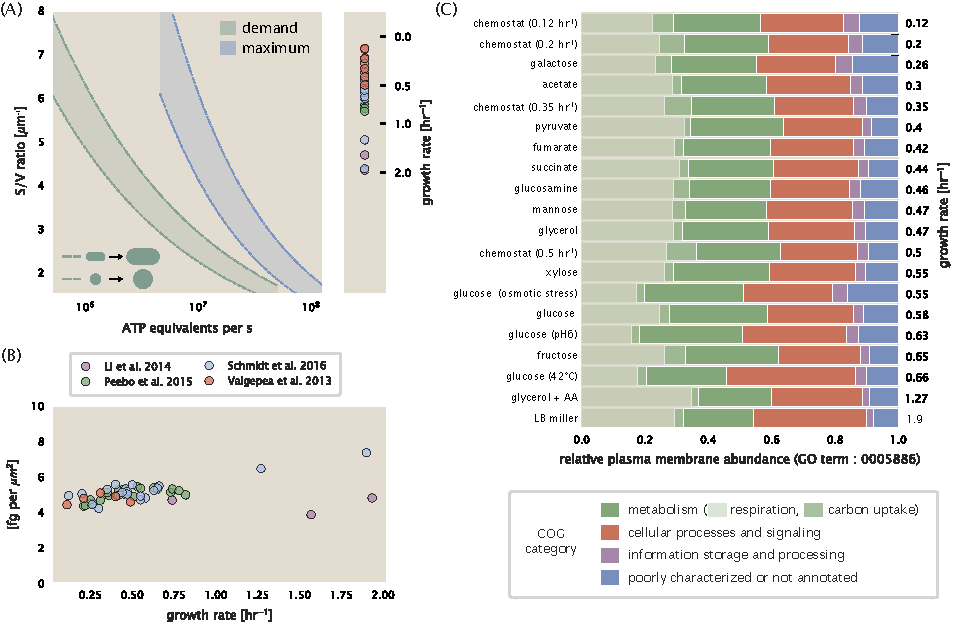
\includegraphics{main_figs/fig5_energy_SV_scaling.pdf}
            \caption{\textbf{Influence of cell size and surface area to volume
            (S/V) ratio on ATP production and inner membrane composition.} (A) Scaling
            of ATP demand and maximum ATP production through respiration as a
            function of S/V ratio. Cell volumes of 0.5 fL to 50 fL were
            considered, with the dashed (\texttt{- -}) line corresponding to a
            sphere and the dash-dot line (\texttt{-.}) reflecting a rod-shaped
            bacterium like \textit{E. coli} with a typical aspect ratio (length
            / width) of 4 \citep{shi2018}. The ATP demand is calculated as
            $10^6$ ATP/(\textmu m$^3$ s), while the maximum ATP production rate
            is taken to be 3 ATP / (nm$^2 \cdot$s)
            \citep{szenk2017}, with calculations of \textit{E. coli} volume and
            surface area detailed in Appendix \nameref{sec:protein_size_SV}. In
            this calculation, 50\% of the bacterial inner membrane is assumed to
            be protein, with the remainder lipid. (B) Total protein mass per
            \textmu m$^2$ calculated for proteins with inner membrane annotation
            (GO term: 0005886). (C) Relative protein abundances by mass based on
            COG annotation. Metabolic proteins are further separated into
            respiration (F$_1$-F$_0$ ATP synthase, NADH dehydrogenase I,
            succinate:quinone oxidoreductase, cytochrome bo$_3$ ubiquinol
            oxidase, cytochrome bd-I ubiquinol oxidase) and carbohydrate
            transport (GO term: GO:0008643). Note that the elongation factor
            EF-Tu can also associate with the inner membrane, but was excluded
            in this analysis due to its high relative abundance (roughly
            identical to the summed protein shown in part
            (B)).}\label{fig:energy_scaling}
            }
                \end{fullwidth}
\end{figure}

% \section{Synthesis of the Cell Envelope}
The subjects of our estimates thus far have been localized to the periphery of
the cell, embedded within the hydrophobic lipid bilayer of the inner membrane.
As outlined in \FIG{energy_scaling}, cells could in principle increase the
expression of the membrane-bound ATP synthases and electron transport chains to
support a larger energy budget across a wide range of cell volumes and membrane
surface areas. This ability, however, is contingent on the ability for the cell
to expand the surface area of the cell by synthesizing new lipids as well as
expanding the peptidoglycan cell wall. In this next class of estimates, we will
turn our focus to these process and consider the copy numbers of the relevant
proteinaceous components needed to synthesize lipids and form new cell wall
material. 

\subsection{Lipid Synthesis}
The cell envelopes of gram negative bacteria (such as \textit{E. coli}) are
composed of an inner and outer phospholipid bilayer membrane separated by a
$\approx 10$ nm periplasmic space. As mentioned in our discussion of the
surface area to volume constraints on energy production, \textit{E. coli} is
a rod-shaped bacterium with a 4:1 length-to-width aspect ratio. At modest
growth rates, such as our stopwatch of 5000 s, the total cell surface area is
$\approx$ 5 \textmu m$^2$ (BNID: 101792, \cite{milo2010}). As there are two
membranes, each of which composed of two lipid leaflets, the total membrane
area is $\approx 20$\textmu m$^2$, a remarkable value compared to the
$\approx$ 2\textmu m length of the cell.

While this represents the total area of the membrane, this does not mean that it
is composed entirely of lipid molecules. Rather the dense packing of the
membrane with proteins means that only $\approx$ 40 \% of the membrane area is
occupied by lipids (BNID: 100078, \cite{milo2010}). Using a rule-of-thumb of 0.5
nm$^2$ as the surface area of the typical lipid (BNID: 106993, \cite{milo2010}),
we arrive at an estimate of $\approx$ 2 $\times$ 10$^7$ lipids per cell, an
estimate in close agreement with experimental measurements (BNID: 100071,
102996; \cite{milo2010}).

The membranes of \textit{E. coli} are composed of a variety of different
lipids, each of which unique in their structures and biosynthetic pathways
\citep{sohlenkamp2016}. With such diversity in biosynthesis, it becomes
difficult to identify which step(s) may be the rate-limiting reactions. This
objective is further complicated by sparsity of \textit{in vivo} kinetic
data. Recently, a combination of stochastic kinetic modeling
\citep{ruppe2018} and \textit{in vitro} kinetic measurements
\citep{ranganathan2012, yu2011} have revealed remarkably slow steps in the
fatty acid synthesis pathways which may serve as the rate limiting reactions.
One such step is the removal of hydroxyl groups from the fatty-acid chain by
ACP dehydratase, leading to the formation of carbon-carbon double bonds. This
reaction, catalyzed both by proteins FabZ and FabA in \textit{E. coli}
\citep{yu2011}, have been estimated to have kinetic turnover rates of
$\approx$ 1 dehydration per second per enzyme \citep{ruppe2018}. Combining
this rate estimate, our previous estimates for the number of lipids to be
formed, and a 5000 second division yields and estimate that the cell requires
$\approx$ 4000 ACP dehydratases. This estimate is in reasonable agreement with the experimentally observed copy
numbers of FabZ and FabA (\FIG{cell_envelope}(A)). Furthermore, we can extend
this estimate to account for the change in membrane surface area as a function
of the growth rate (grey line in \FIG{cell_envelope}(A)), which captures the
observed growth rate dependent expression of these two enzymes. 

Despite the slow catalytic rate of the FabZ and FabA enzymes, we argue that the
generation of fatty acids is not a bottleneck in cell division and is not the
key process responsible for setting the bacterial growth rate. Experimental
evidence has shown that the rate of fatty-acid synthesis can be drastically
increased \textit{in vitro} by increasing the concentration of FabZ
\cite{yu2011}. Stochastic simulations of the complete fatty acid synthesis
pathway of \textit{E. coli} further supports this experimental observation
\cite{ruppe2018}. Thus, if this step was the determining factor in cell
division, increasing growth rate could be as simple as increasing the number of
ACP dehydratases per cell. With a proteome size of $\approx$ 3$\times$10$^6$
proteins, a drastic increase in expression from 4000 to 40,000 ACP dehydratases
would result in a $\approx$ 1\% increase in the proteome pool. As other proteins
such as ribosomes and tRNA synthetases are in much larger
abundance than 4000 per cell (as we will see in the coming sections), it is
unlikely that expression of ACP dehydratases couldn't be increased to facilitate
faster growth.


\begin{figure}
    \begin{fullwidth}
    \centering{
        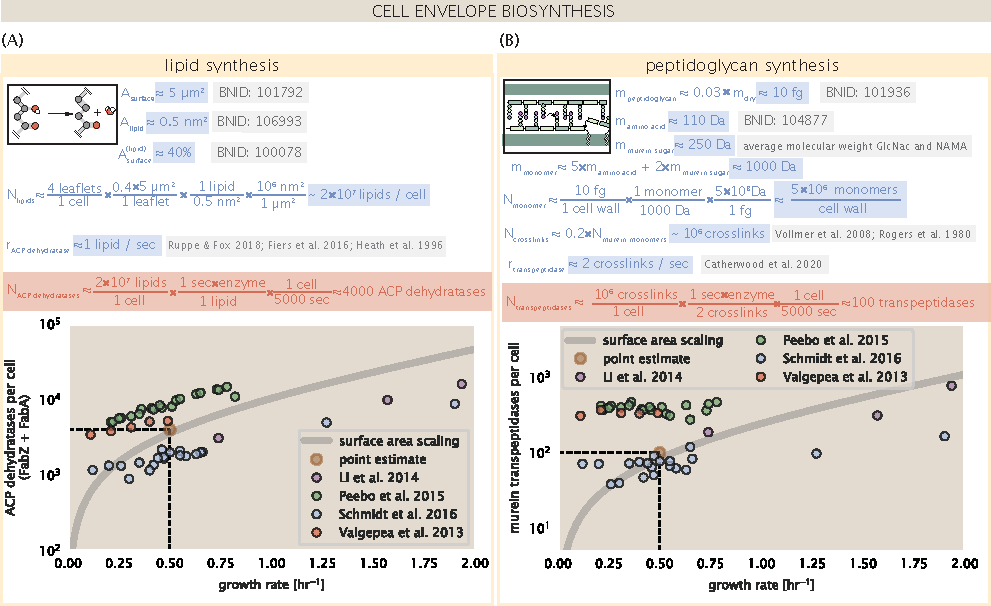
\includegraphics{main_figs/cell_wall_peptidoglycan.pdf}
        \caption{\textbf{Estimation of the key components involved in cell
        envelope biosynthesis.} (A) Top panel shows a schematic estimation for
        the number of ACP dehydratases necessary to form functional
        phospholipids. The rate of ACP dehydratases was inferred from
        experimental measurements via a stochastic kinetic model described in
        \cite{ruppe2018}. Bottom panel shows the experimentally observed complex
        copy numbers using the stoichiometries [FabA]$_2$ and [FabZ]$_2$. (B) An
        estimate for the number of peptidoglycan transpeptidases needed to
        complete maturation of the peptidoglycan. The mass of the murein monomer
        was estimated by approximating each amino acid in the pentapeptide chain
        as having a mass of 110 Da and each sugar in the disaccharide having a
        mass of $\approx$ 250 Da. The \textit{in vivo} rate of transpeptidation
        rein \textit{E. coli} was taken from recent analysis by
        \cite{catherwood2020}. The bottom panel shows experimental measurements
        of the transpeptidase complexes in \textit{E. coli} following the
        stoichiometries [MrcA]$_2$, [MrcB]$_2$, [MrdA]$_1$, and [MrdB]$_1$. Grey
        curves in each plot show the estimated number of complexes needed to
        satisfy the synthesis requirements scaled by the surface area as a
        function of growth rate. We direct the reader to the supplemental
        information for a more detailed discussion of this estimate. 
        }
        \label{fig:cell_envelope}
    }
    \end{fullwidth}

\end{figure}


\subsection{Peptidoglycan Synthesis}
While variation in cell size as a function growth rate can be large,
bacterial cells demonstrate exquisite control over their cell shape. The
maintenance of cell shape is due primarily to the intricate meshwork of the
cell wall, a shell of polymerized discaccharides interspersed with short
peptide crosslinks termed the peptidoglycan. In gram negative bacteria, such as \textit{E. coli}, this
enormous peptidoglycan molecule is a few nanometers thick and resides within the
periplasmic space between the inner and outer membrane. The formation of the
peptidoglycan is an intricate process, involving the bacterial actin homolog
MreB \citep{shi2018} along with a variety of membrane-bound and periplasmic
enzymes \citep{morgenstein2015}. The coordinated action of these components
result in a highly-robust polymerization framework which maintains cell shape
even in the face of large-scale perturbations and can restore rod-shaped
morphology even after digestion of the peptidoglycan \citep{harris2018,shi2018}.

In glucose-supported balanced growth, the peptidoglycan alone comprises
$\approx$ 3\% of the cellular dry mass (BNID: 101936, \cite{milo2010}), making it the most massive molecule in
\textit{E. coli}. The polymerized unit of the peptidoglycan is a
N-acetylglucosamine and N-acetylmuramic acid disaccharide, the former of which
is functionalized with a short pentapeptide. With a mass of $\approx$ 1000 Da,
this unit, which we refer to as a murein monomer, is polymerized to form long
strands in the periplasm which are attached to eachother via the peptide linkers. Using the
aforementioned measurement that $\approx$ 3\% of the dry mass is peptidoglycan,
it can be estimated that the peptidoglycan is composed of $\approx$
6$\times$10$^6$ murein monomers.

In principle, each one of these murein monomers can be crosslinked to another
glycan strand via the pentapeptide. In some species, such as in gram-positive
bacterium \textit{Staphylococcus aureus}, the extent of crosslinking can be
large with $>$ 90\% of pentapeptides forming a connection between glycan
strands. In \textit{E. coli}, however, a much smaller proportion ($\approx$
20\%) of the peptides are crosslinked, resulting in a weaker and more porous
cell wall \cite{vollmer2008a, rogers1980}. The formation of these crosslinks
primarily occur during the polymerization of the murein monomers and is
facilitated by a family of enzymes called transpeptidases. In \textit{E. coli},
there are four primary transpeptidases that are involved in lateral and
longitudinal extension of the peptidoglycan. These transpeptidases have only
recently been quantitatively characterized \textit{in vivo} via liquid
chromatography mass spectrometry \citep{catherwood2020}, which revealed a
kinetic turnover rate of $\approx 1 - 2$ crosslinking reactions formed per
second per enzyme.

Pulling these measurements together permits us to make an estimate that on the
order of $\approx$ 100 transpeptidases are needed for complete maturation of the
peptidoglycan, given a division time of $\approx$ 5000 seconds, a value that is
closely aligned with the experimental observations (\FIG{cell_envelope}(B)). Expanding this
estimate to account for the changing volume of the peptidoglycan as a function
of growth rates (grey line in \FIG{cell_envelope}(B)) also qualitatively captures the observed
dependence in the data, though systematic disagreements between the different
data sets makes the comparison more difficult. 

Much as in the case of fatty acid synthesis, we find it unlikely that the
formation of peptidoglycan is a rate limiting step in bacterial cell division.
The estimate we have presented considers only the transpeptidase enzymes that
are involved lateral and longitudinal elongation of the peptidoglycan (proteins
MrdA, MrdB, MrcA, and MrcB). This neglects the presence of other transpeptidases
that are present in the periplasm that are involved in remodeling and maturation
of the peptidoglycan. It is therefore possible that if this was setting the
speed limit for cell division, the simple expression of more maturation
transpeptidases may be sufficient to maintain the structural integrity of the
cell wall. 

Furthermore, it has been shown experimentally that, while critical for cell
wall formation, there are components needed beyond  the transpeptidases to
maintain cell shape and permit cell division. For example, the bacterial actin
homolog MreB polymerizes laterally along the inner membrane and facilitates the
longitudinal expansion of the peptidoglycan. Inhibition of MreB through the
addition of small molecules results in loss of the cell shape, though formation
of the peptidoglycan is not significantly hindered \cite{shi2018}. This suggests
that in considering the development of the cell envelope, proper assembly may
be a more important property to consider beyond synthesis of the appropriate
number of glycan polymers. 
% \section{Processes of the Central Dogma}
Up to this point, we have considered a variety of transport and biosynthetic
processes that are critical to acquiring and generating new cell mass. While
there are of course many other metabolic processes we could consider, we now
turn our focus to some of the most important processes which \textit{must} be
undertaken irrespective of the growth conditions -- those of the central
dogma.

\subsection{DNA Replication}
Most bacteria (including \textit{E. coli}) harbor a single, circular chromosome
and can have extra-chromosomal plasmids up to $\sim$ 100 kbp in length. While
we consider the starting material dNTPs in \FIGSUPP[DNA_synthesis]{dntp} and
discussed further in the Appendix Section "\nameref{sec:SI_central_dogma}", here we focus
our quantitative thinking on the chromosome of \textit{E. coli}, which
harbors $\approx$ 5000 genes and $\approx 5\times 10^6$ base pairs.

To successfully divide and produce viable progeny, this chromosome must be
faithfully replicated and segregated into each nascent cell. Replication is
initiated at a single region of the chromosome termed the \textit{oriC} locus
where a pair of replisomes, each consisting of two DNA polymerase III,
begin their high-fidelity replication of the genome in opposite directions
\citep{fijalkowska2012}. \textit{In vitro} measurements have shown that DNA
Polymerase III copies DNA at a rate of $\approx 600$ nucleotides per second
(BNID: 104120). Therefore, to replicate a single chromosome, two replisomes
moving at their maximal rate would copy the entire genome in $\approx$ 4000
s. Thus, with a division time of 5000 seconds, there is sufficient time for a pair
of replisomes complexes to replicate the entire genome.

\begin{figure}
  \centering{
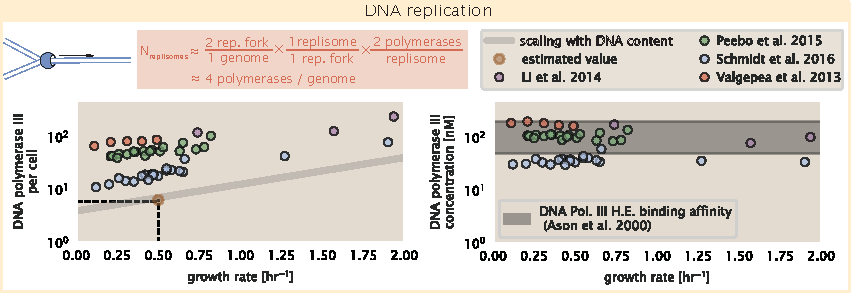
\includegraphics{main_figs/fig6_DNA_replication_main.pdf}
\caption{\textbf{Complex abundance estimates for dNTP synthesis and DNA
replication.} An estimate
for the minimum number of DNA polymerase holoenzyme complexes needed to
facilitate replication of a single genome. Points in the left-hand plot correspond
to the total number of DNA polymerase III holoenzyme complexes
([DnaE]$_3$[DnaQ]$_3$[HolE]$_3$[DnaX]$_5$[HolB][HolA][DnaN]$_4$[HolC]$_4$[HolD]$_4$)
per cell. Right-hand plot shows the effective concentration of DNA polymerase III
holoenzyme (See Appendix \nameref{sec:protein_size_SV} for calculation of cell
size). Grey lines in left-hand panel show the estimated number of
complexes needed as a function of growth, the details of which are described
in the Supplemental Information.} \label{fig:DNA_synthesis}
 }
\figsupp[Estimate and observations of the abundance of ribonucleotide
reductase, a key component in dNTP synthesis.]{Estimate of the number of
ribonucleotide reductase enzymes needed to facilitate the synthesis of
$\approx 10^7$ dNTPs over the course of a 5000 second generation time. Points
in the plot correspond to the total number of ribonucleotide reductase I
([NrdA]$_2$[NrdB]$_2$) and ribonucleotide reductase II ([NrdE]$_2$[NrdF]$_2$)
complexes. Grey lines in top panel show the estimated number of complexes
needed as a function of growth, the details of which are described in the
Appendix.}{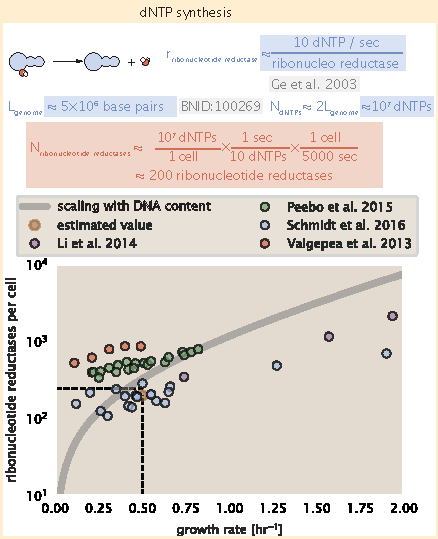
\includegraphics{main_figs/fig6-S1_dNTP_synthesis.pdf}}\label{figsupp:dntp}

\end{figure}

In rapidly growing cultures, bacteria like \textit{E. coli}
can initiate as many as 10 - 12 replication forks at a
given time \citep{bremer2008, si2017},  we expect only a few DNA polymerases
($\approx 10$) are needed. However, as shown in \FIG{DNA_synthesis}, DNA
polymerase III is nearly an order of magnitude more abundant. This discrepancy
can be understood by considering its binding constant to DNA. \textit{In vitro} characterization has quantified the $K_D$ of
DNA polymerase III holoenzyme to single-stranded and double-stranded DNA to be
50 and 200 nM, respectively \citep{ason2000}. The right-hand plot in
\FIG{DNA_synthesis} shows that the concentration of DNA polymerase III
across all data sets is within this range. Thus, its copy number appears to vary such that its
concentration is approximately equal to the dissociation constant to the DNA.
While the processes regulating the initiation of DNA replication are complex and
involve more than just the holoenzyme, these data indicate that the kinetics of
replication rather than the explicit copy number of the DNA polymerase III
holoenzyme is the more relevant feature of DNA replication to consider. In light
of this, the data in \FIG{DNA_synthesis} suggests that for bacteria like
\textit{E. coli}, DNA replication does not represent a rate-limiting step in
cell division. However, it is worth noting that for bacterium like \textit{C.
crescentus} whose chromosomal replication is initiated only once per cell cycle
\citep{jensen2001}, the time to double their chromosome indeed represents an
upper limit to their growth rate.

% \subsection{RNA Synthesis}\label{sec:RNA_synthesis}
With the machinery governing the replication of the genome accounted for, we
now turn our attention to the next stage of the central dogma -- the
transcription of DNA to form RNA. We primarily consider three major groupings
of RNA, namely the RNA associated with ribosomes (rRNA), the RNA encoding the
amino-acid sequence of proteins (mRNA), and the RNA which links codon
sequence to amino-acid identity during translation (tRNA). Despite the varied
function of these RNA species, they share a commonality in that they are
transcribed from DNA via the action of RNA polymerase. In the coming
paragraphs, we will consider the synthesis of RNA as a rate limiting step in
bacterial division by estimating how many RNA polymerases must be present to
synthesize all necessary rRNA, mRNA, and tRNA.

\subsubsection{rRNA}
We begin with an estimation of the number of RNA polymerases needed to
synthesize the rRNA that serve as catalytic and structural elements of the
ribosome. Each ribosome contains three rRNA molecules of lengths 120, 1542,
and 2904 nucleotides (BNID: 108093, \cite{milo2010}), meaning each ribosome
contains $\approx$ 4500 nucleotides. As the \textit{E. coli} RNA polymerase
transcribes DNA to RNA at a rate of $\approx$ 40 nucleotides per second
(BNID: 101904, \cite{milo2010}), it takes a single RNA polymerase
$\approx$ 100 s to synthesize the RNA needed to form a single functional ribosome.
Therefore, in a 5000 s division time, a single RNA polymerase transcribing
rRNA at a time would result in only $\approx$ 50 functional ribosomal rRNA
units -- far below the observed number of $\approx 10^4$ ribosomes per cell.

Of course, there can be more than one RNA polymerase transcribing the rRNA genes
at any given time. To elucidate the \textit{maximum} number of rRNA units that can
be synthesized given a single copy of each rRNA gene, we will consider a
hypothesis in which the rRNA operon is completely tiled with RNA polymerase.
\textit{In vivo} measurements of the kinetics of rRNA transcription have revealed that
RNA polymerases are loaded onto the promoter of an rRNA gene at a rate of
$\approx$ 1 per second (BNID: 111997; 102362, \cite{milo2010}). If RNA
polymerases are being constantly loaded on to the rRNA genes at this rate,
then we can assume that $\approx$ 1 functional rRNA unit is
synthesized per second. With a 5000 second division time, this hypothesis
leads to a maximal value of 5000 functional rRNA units, still undershooting
the observed number of $10^4$ ribosomes per cell.

\textit{E. coli}, like many other bacterium, have evolved a clever mechanism to surpass this kinetic limit
for the rate of rRNA production. Rather than having only one copy of each rRNA
gene, \textit{E. coli} has seven copies of the operon (BIND: 100352,
\cite{milo2010}) four of which are localized directly adjacent to the origin of
replication \citep{birnbaum1971}. As fast growth also implies an increased gene
dosage due to paralellized chromosomal replication, the total number of rRNA
genes can be on the order of $\approx$ 10 -- 70 copies at moderate to fast
growth rates \citep{stevenson2004}. Using our standard time scale of a 5000
second division time, we can make the lower-bound estimate that the typical cell
will have 7 copies of the rRNA operon. Synthesizing one functional rRNA unit per
second per rRNA operon, a total of $4 \times 10^4$ rRNA units can be
synthesized, comfortably above the observed number of ribosomes per cell.

How many RNA polymerases are then needed to constantly transcribe 7 copies of
the rRNA genes? We approach this estimate by considering the maximum number
of RNA polymerases tiled along the rRNA genes with a loading rate of 1 per
second and a transcription rate of 40 nucleotides per second. Considering
that a RNA polymerase has a physical footprint of approximately 40
nucleotides (BNID: 107873, \cite{milo2010}), we can expect
$\approx$ 1 RNA polymerase per 80 nucleotides. With a total length of
$\approx$ 4500 nucleotides per operon and 7 operons per cell, the maximum
number of RNA polymerases that can be transcribing rRNA at any given time is
$\approx$ 400. As we will see in the coming sections, the
synthesis of rRNA is the dominant requirement of the RNA polymerase pool.

\subsubsection{mRNA}
To form a functional protein, all protein coding genes must first be
transcribed from DNA to form an mRNA molecule. While each protein requires an
mRNA blueprint, many copies of the protein can be synthesized from a single
mRNA. Factors such as strength of the ribosomal binding site, mRNA stability,
and rare codon usage frequency dictate the number of proteins that can be
made from a single mRNA, with yields ranging from 10$^1$ to 10$^4$ (BNID: 104186; 100196;
106254, \cite{milo2010}). Computing the geometric mean of this range yields
$\approx$ 1000 proteins synthesized per mRNA, a value that agrees with
experimental measurements of the number of proteins per cell ($\approx 3
\times 10^6$, BNID: 100088, \cite{milo2010}) and total number of mRNA per
cell ($\approx 3 \times 10^3$, BNID:100064, \cite{milo2010}).

This estimation captures the \textit{steady-state} mRNA copy number, meaning
that at any given time, there will exist approximately 3000 unique mRNA
molecules. To determine the \textit{total} number of mRNA that need to be
synthesized over the cell's lifetime, we must consider degradation of the mRNA.
In most bacteria, mRNAs are rather unstable with life times on the order of
several minutes (BNID: 104324; 106253; 111927; 111998, \cite{milo2010}). For
convenience, we assume that the typical mRNA in our cell of interest has a
typical lifetime of $\approx$ 300 seconds. Using this value, we can determine
the total mRNA production rate to maintain a steady-state copy number of 3000
mRNA per cell. While we direct the reader to the appendix for a more detailed
discussion of mRNA transcriptional dynamics, we state here that the total mRNA
production rate must be on the order of $\approx$ 15 mRNA per second. In
\textit{E. coli}, the average protein is $\approx$ 300 amino acids in length
(BNID: 108986; \cite{milo2010}), meaning that the corresponding mRNA is
$\approx$ 900 nucleotides which we will further approximate as $\approx$ 1000
nucleotides to account for the non-protein coding regions on the 5' and
3' ends. This means that the cell must have enough RNA polymerase molecules
about to sustain a transcription rate of $\approx 1.5 \times 10^4$ nucleotides
per second. Knowing that a single RNA polymerase polymerizes RNA at a clip of 40
nucleotides per second, we arrive at a comfortable estimate of $\approx$ 250 RNA
polymerase complexes needed to satisfy the mRNA demands of the cell. It is worth
noting that this number is approximately half of that required to synthesize
enough rRNA, as we saw in the previous section. We find this to be a striking
result as these 250 RNA polymerase molecules are responsible for the
transcription of the $\approx$ 4000 protein coding genes that are not ribosome
associated.

\subsubsection{tRNA}
The final class of RNA molecules worthy of quantitative consideration are the
tRNAs that are used during translation to map codon sequence on mRNA to specific amino acids.
Unlike mRNA or rRNA, each individual tRNA is remarkably short, ranging
from 70 to 95 nucleotides each (BNID: 109645; 102340, \cite{milo2010}). What
they lack in length, they make up for in abundance, with reported values ranging from
$\approx$6$\times$10$^4$ (BNID: 105280, \cite{milo2010}) to
$\approx$4$\times$10$^5$ (BNID: 108611). To test tRNA synthesis as a possible
growth-rate limiting stage, we will err towards a higher abundance of $\approx$
4$\times$10$^5$ per cell. Combining the abundance and tRNA length measurements,
we make the estimate that $\approx 5 \times 10^7$ nucleotides are sequestered in tRNA per cell.
Unlike mRNA, tRNA is remarkably stable with typical lifetimes \textit{in vivo}
on the order of $\approx$ 48 hours \citep{abelson1974,svenningsen2017} -- well
beyond the timescale of division. Once again using our rule-of-thumb for the
rate of transcription to be 40 nucleotides per second and assuming a division
time of $\approx$ 5000 seconds, we arrive at an estimate of $\approx$ 150 RNA
polymerases to synthesize enough tRNA. This requirement pales in comparison to
the number of polymerases needed to generate the rRNA and mRNA pools and can be
neglected as a significant transcriptional burden.

\begin{figure}
    \begin{fullwidth}
    \centering{
        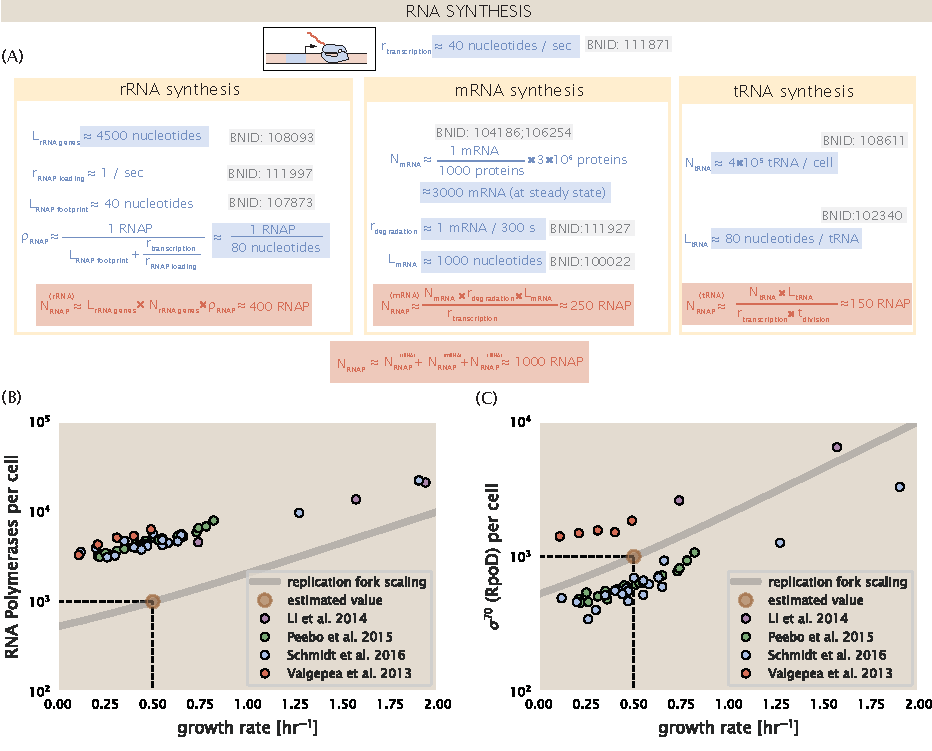
\includegraphics{main_figs/fig7_RNA_synthesis.pdf}
        \caption{\textbf{Estimation of the RNA polymerase demand and
        comparison with experimental data.} (A) Estimations for the number of
        RNA polymerase needed to synthesize sufficient quantities of rRNA, mRNA,
        and tRNA from left to right, respectively. Bionumber Identifiers (BNIDs)
        are provided for key quantities used in the estimates. (B) The RNA
        polymerase core enzyme copy number as a function of growth rate. Colored
        points correspond to the average number RNA polymerase core enzymes that
        could be formed given a subunit stoichiometry of [RpoA]$_2$[RpoC][RpoB].
        (C) The abundance of $\sigma^{70}$ as a function of growth rate.
        Estimated value for the number of RNAP is shown in (B) and (C) as a
        translucent brown point at a growth rate of 0.5 hr$^{-1}$.}
    \label{fig:RNA_synthesis}
    }
    \end{fullwidth}
\end{figure}


\subsubsection{RNA Polymerase and $\sigma$-factor Abundance}
These estimates, summarized in \FIG{RNA_synthesis} (A), reveal that synthesis of
rRNA  and mRNA are the dominant RNA species synthesized by RNA polymerase,
suggesting the need for $\approx$ 700 RNA polymerases per cell. As is revealed
in \FIG{RNA_synthesis} (B), this estimate is about an order of magnitude below
the observed number of RNA polymerase complexes per cell ($\approx$ 5000 -
7000). The disagreement between the estimated number of RNA polymerases and
these observations are at least consistent with recent literature revealing that
$\approx$ 80 \% of RNA polymerases in \textit{E. coli} are not transcriptionally
active \citep{patrick2015}. Our estimate ignores the possibility that some
fraction is only nonspecifically bound to DNA, as well as the obstacles that RNA
polymerase and DNA polymerase present for each other at they move along the DNA
\citep{finkelstein2013}.

In addition, it is also vital to consider the role of $\sigma$-factors which
help RNA polymerase identify and bind to transcriptional start sites
\citep{browning2016}. Here we consider $\sigma^{70}$ (RpoD) which is the
dominant "general-purpose" $\sigma$-factor in \textit{E. coli}. While initially
thought of as being solely involved in transcriptional initiation, the past two
decades of single-molecule work has revealed a more multipurpose role for
$\sigma^{70}$ including facilitating transcriptional elongation
\citep{kapanidis2005, goldman2015, perdue2011,mooney2003,mooney2005}.
\FIG{RNA_synthesis} (B) is suggestive of such a role as the number of
$\sigma^{70}$ proteins per cell is in close agreement with our estimate of the
number of transcriptional complexes needed.

These estimates provide insight as to the observed magnitude of both RNA
polymerase and the $\sigma$-70 factor. As we have done in the previous sections,
and described in the supplemental information, we can generalize these estimates
across a wide range of growth rates (grey line in \FIG{RNA_synthesis}(B). While
there remains some disagreement in the magnitude of the copy number, this
estimate appears to very adequately describe the growth rate dependence of these
complexes. Furthermore, these findings illustrate that transcription
cannot be the rate limiting step in bacterial division. \FIG{RNA_synthesis} (A)
reveals that the availability of RNA polymerase is not a limiting factor for
cell division as the cell always has an apparent $\sim$ 10-fold excess than needed.
Furthermore, if more transcriptional activity was needed to satisfy the cellular
requirements, more $\sigma^{70}$-factors could be expressed to utilize a larger
fraction of the RNA polymerase pool.

\section{Protein synthesis}

Lastly, we turn our attention to the process of translation. So far our
estimates have led to protein copy numbers that are consistent with the
proteomic data, or even in excess of what might be needed for each task under
limiting growth conditions. Even in our example of \textit{E. coli} grown under
different carbohydrate sources (\FIG{carbon_tport}(B)), cells can utilize
alternative carbon sources by inducing the expression of additional membrane
transporters and enzymes. Optimal resource allocation and the role of ribosomal
proteins have been an area of intense quantitative study over the last decade by
Hwa and others \citep{scott2010, hui2015}. From the perspective of limiting
growth, our earlier estimate of rRNA highlighted the necessity for multiple
copies of rRNA genes in order to make enough rRNA, suggesting the possibility
that synthesis of ribosomes might be rate limiting. While the transcriptional
demand for  the ribosomal proteins is substantially lower than rRNA genes, since
many proteins can be translated from relatively fewer mRNA, other ribosomal
proteins like the translation elongation factor EF-Tu also present a substantial
burden. For EF-Tu  in particular, it is the most highly expressed protein in
\textit{E. coli} and  is expressed by multiple genes on the chromosome, tufA and
tufB.

% Experimentally,
% consecutive deletion of rRNA operons showed a significant reduction in growth
% rate in rich media when cells had only 3 or less \citep{levin2017}.

% Separately, it has been found that gross
% overexpression of a protein can dramatically lower growth rate due to the
% altered allocation of resources \citep{basan2015}.

We begin by first estimating the number of tRNA synthetases and ribosomes
required for  a doubling time of 5000 seconds.  \textit{E. coli} has roughly 3 x
10$^6$ proteins per cell, which for an average protein of 300 aa, amounts to the formation
of $\approx$ 10$^9$ peptide bonds. This also corresponds to the
number of amino-acyl tRNA that are used by ribosomes, with the pool of tRNA continuously
recharging new amino acids by tRNA synthetases. At a rate of charging of
about 20 amino-acyl tRNA per second (BNID: 105279, \cite{milo2010}), we find
that cells have more than sufficient tRNA synthetases to meet the demand of
ribosomes during  protein synthesis (\FIG{protein_synthesis}(A)).
If we consider an elongation rate of $\approx$ 15 peptide bonds per second
(BNID: 114271, \cite{milo2010, dai2016}), the formation of $\approx$ 10$^9$
peptide bonds would require 1.5 x 10$^4$ ribosomes at a growth rate of 0.5
hr$^{-1}$. This is indeed consistent with the experimental data shown in
\FIG{protein_synthesis}(B).

[NB: How about moving this estimates paragraph and associated \FIG{protein_synthesis} to SI after all?]

\begin{figure}
    \begin{fullwidth}
    \centering{
        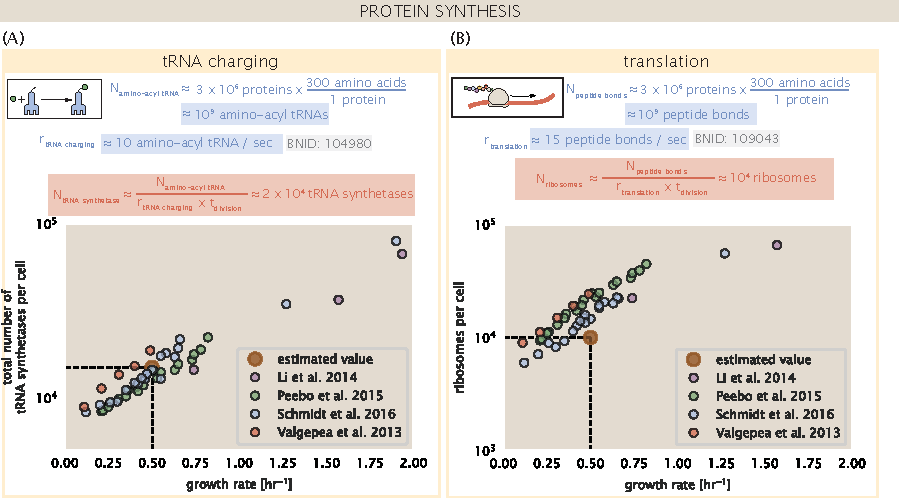
\includegraphics{main_figs/protein_synthesis.pdf}
        \caption{\textbf{Estimation of the required tRNA synthetases and
        ribosomes.} (A) Estimation for the
        number of tRNA synthetases that will supply the required amino acid
        demand. The sum of all tRNA synthetases copy numbers are plotted as a
        function of growth rate ([ArgS], [CysS], [GlnS], [GltX], [IleS], [LeuS],
        [ValS], [AlaS]$_2$, [AsnS]$_2$, [AspS]$_2$, [TyrS]$_2$, [TrpS]$_2$,
        [ThrS]$_2$, [SerS]$_2$, [ProS]$_2$, [PheS]$_2$[PheT]$_2$, [MetG]$_2$,
        [lysS]$_2$, [HisS]$_2$, [GlyS]$_2$[GlyQ]$_2$). (B) Estimation for the
        number of ribosomes required to synthesize all proteins in the cell. The
        average abundance of ribosomes is plotted as a function of growth rate.
        Our estimated values are shown for a growth rate of 0.5 hr$^{-1}$.}
    \label{fig:protein_synthesis}
    }
    \end{fullwidth}
\end{figure}

We can begin to gain some intuition into how translation might limit growth by
noting that the total number of peptide bonds generated as the cell doubles,
$N_{aa}$, which we used in our calculation above, will be given by, $\tau \cdot
r_t \cdot R$. Here, $\tau$ refers to the doubling time of the cell under
steady-state growth, $r_t$ is the maximum translation elongation rate, and $R$
is the average number of ribosomes per cell. With the growth rate related to the
cell doubling time by $\lambda = ln(2)/\tau$, we can write the
translation-limited growth rate as,

\begin{equation}
\lambda_{\textrm{translation-limited}} = \frac{ln(2) \cdot r_t \cdot R}{N_{aa}}.
\end{equation}
Alternatively, since $N_{aa}$ is related to the total protein mass through the
molecular weight of each protein, we can also consider the growth rate in terms
of ribosomal mass fraction. By making the approximation that an average amino
acid has a molecular weight of 110 Da (see \FIG{translation_1}(A)), we can
rewrite the growth rate as,

\begin{equation}
\lambda_{\textrm{translation-limited}} \approx \frac{ln(2) \cdot r_t}{L_R}  \Phi_R,
\label{eq:translation_limit_growth_rate}
\end{equation}
where $L_R$ is the total length in amino acids that make up a ribosome, and
$\Phi_R$ is the ribosomal mass fraction. This is plotted as a function of
ribosomal fraction $\Phi_R$ in \FIG{translation_1}(A), where we take $L_R
\approx $7459 aa, corresponding to the length in amino acids for all ribosomal
subunits of the 50S and 30S complex. This formulation assumes that the cell can
transcribe the required amount of rRNA, which appears reasonable for  \textit{E.
coli} under the  allowing us to consider the inherent limit on growth set by the
ribosome.

The growth rate defined by Equation \ref{eq:translation_limit_growth_rate}
reflects  mass-balance under steady-state growth and has long provided a
rationalization to the apparent linear increase in \textit{E. coli}'s ribosomal
content as a function of growth rate \citep{Goldberger1979, scott2010}. For our
purposes, there are several important consequences of this  trend. Perhaps the
first thing to notice is that there is a maximum growth rate at about $\lambda
\approx 6 hr^{-1}$, or doubling time of about 7 minutes (dashed line). This
growth rate can be viewed as an inherent maximum growth rate due to the need for
the cell to double the cell's entire ribosomal mass. Interestingly, this limit
is independent of the absolute number of ribosomes, but rather is simply given
by time to translate an entire ribosome, $L_R/ r_t$. As shown in
\FIG{translation_1}(B), we can reconcile this with the observation that in order
to double the average number of ribosomes, each ribosome must produce a second
ribosome. This is a process that cannot be parallelized.

For reasonable values of $\Phi_R$, between about 0.1 - 0.3 \citep{scott2010},
the maximum growth rate is in line with experimentally reported growth rates
around 0.5 - 2 $hr^{-1}$. Here we are implicitly assuming that translation
proceeds randomly, without preference between ribosomal or non-ribosomal mRNA,
which appears reasonable. Importantly, in order for a cell to scale this growth
limit set by $\Phi_R$, cells \textit{must} increase their ribosomal abundance.
This can be achieved by either synthesizing more ribosomes or reducing the
fraction of non-ribosomal proteins. Reduction of non-ribosomal proteins is not
straight forward since, as we have found throughout our estimates, doubling a
cell requires a substantial number of other enzymes and transporters. Increasing
the absolute ribosomal abundance is limited by the number of rRNA operons.

\begin{figure}
  \begin{fullwidth}
        \centering{
            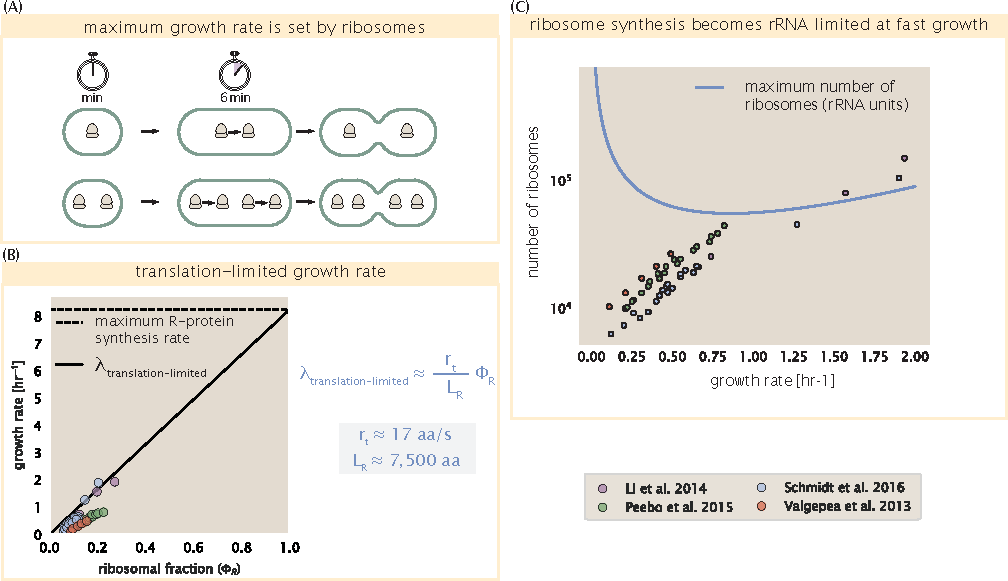
\includegraphics{main_figs/fig7_ribosome_growth_limit_2.pdf}
            \caption{\textbf{Translation-limited growth rate.} (A) Here we
            consider the translation-limited growth as a function of ribosomal
            fraction. By mass balance, the time required to double the entire
            proteome ($N_{aa}$ /$r_t \cdot $) sets the translation-limited
            growth rate, $\lambda_{\textrm{translation-limited}}$. Here $N_{aa}$
            is effectively the number of peptide bonds that must be translated,
            $r_t$ is the translation elongation rate, and $R$ is the number of
            ribosomes. This can also be re-written in terms of the ribosomal
            mass fraction $\Phi_R = m_R$ / $m_{\textrm{protein}}$, where $m_R$
            is the total ribosomal mass and $m_{\textrm{protein}}$ is the mass
            of all proteins in the cell. $L_R$ refers to the summed length of
            the ribosome in amino acids.
            $\lambda_{\textrm{translation-limited}}$ is ploted as a function of
            $\Phi_R$ (solid line). (B) The dashed line in part (A) identifies a
            maximum growth rate that is set by the ribosome. Specifically, this
            growth rate corresponds to the time required to  translation an
            entire ribosome, $L_R/ r_t$ . This is a result that is independent
            of the number of ribosomes in the cell as shown schematically here.
            (C) Schematic showing translation-specific requirements for maintenance
            of steady-state growth. In a nutrient rich environment, amino acid supply $r_{aa}$ is sufficiently in
            excess of demand by ribosomes translating at their maximal rate. In poorer
            nutrient conditions, reduced amino acid supply $r_{aa}$ will decrease
            the rate of elongation. In a regime where $r_{aa}$ is less than $r_t \cdot R$,
            the number of actively translating ribosomes will need to be reduced in order
            to maintain steady-state growth.}
        \label{fig:translation_1}
        }
  \end{fullwidth}
\end{figure}

While it is common for bacteria to decrease their ribosomal abundance in poorer
nutrient conditions \cite{scott2010, liebermeister2014}, this does not decrease
to zero. From the perspective of a bacterium dealing with uncertain nutrient
conditions, there is likely a benefit for the cell to maintain some relative
fraction of ribosomes to support rapid growth as nutrient conditions improve.
However, if we consider a scenario where nutrient conditions become poorer and
poorer, there will be a regime where ribosomes are in excess of the nutrient
supply. If the cell is to maintain steady-state growth, it will need to
attenuate its translational activity since ribosomes would otherwise exhaust
their supply of amino acids and bring cell growth to a halt
(\FIG{translation_1}(C)). In the next section we will consider this more
specifically for \textit{E. coli}, which has been shown to maintain a relatively
high elongation rate even in stationary phase ($\approx$ 8 aa/s, \cite{dai2016})
where cell growth is minimal.

[NB: I'm considering moving this paragraph near the end of the next section].

% In addition,
% given their massive size at about 850 kDa, they may play an as-yet fully
% understood role as a crowding agent in cellular function \cite{delarue2018,
% solerbistue2020}.

\subsection{Multiple replication forks bias ribosome abundance.}

\textit{E. coli} cells grow by an adder mechanism, whereby cells add a constant
volume with each cell division \citep{taheriaraghi2015}. In conjunction with
this, additional rounds of DNA replication are triggered when cells reach a
critical volume per origin of replication (\FIG{translation_ecoli}(A)). This
leads to the classically-described exponential increase in cell size with growth
rate \cite{schaechter1958, si2017, si2019}. In the context of maximizing growth
rate, it is notable that the majority of ribosomal proteins and rRNA operons are
found closer to the DNA origin. Given the need to increase to total gene dosage
of rRNA operons at faster growth rates, and the intimate relationship between ribosomal
content and growth rate we considered above, this raises the possibility that the
observed size scaling and increase in chromosomal content might simply be
a means for the cell to tune biosynthesis according to its
physiological state.

While an increase in transcription has been observed for genes near the origin
in rapidly growing \textit{E. coli}  \citep{scholz2019}, we were unaware of such
characterization at the proteomic level. In order to test whether there is a
relative increase in protein expression for genes closer to the origin, we
calculated a running boxcar average of protein copy number as a function of
each gene's transcriptional start site. While absolute protein copy numbers can vary
substantially across the chromosome, we indeed observe a bias in expression
under fast growth conditions (\FIG{translation_ecoli}(B), showing the result
using a 0.5 kb averaging window). The dramatic change in protein copy number
near the origin mainly reflects the increase in ribosomal protein expression.
This trend is in contrast to slower growth conditions where the average copy
number is more uniform across the length of the chromosome.

\begin{figure*}
    \begin{fullwidth}
    \centering{
        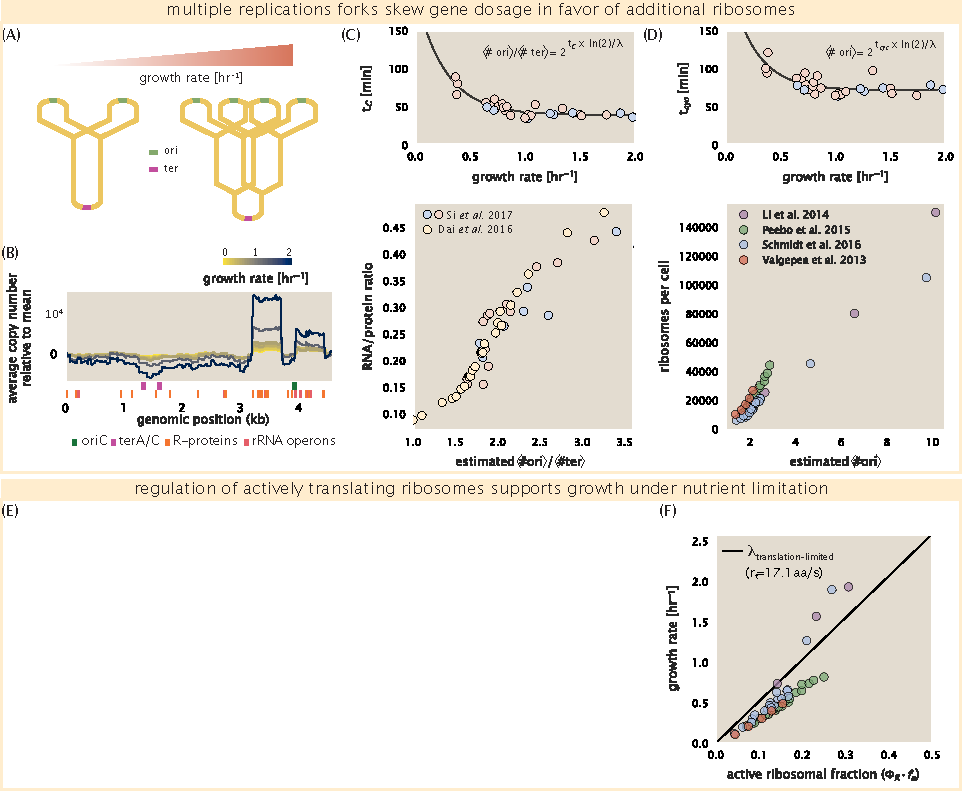
\includegraphics{main_figs/fig8_ribosome_growth_limit_ecoli_temp.pdf}
        \caption{\textbf{Multiple replication forks skew gene dosage and
        ribosomal content.} (A) Schematic shows the expected
        increase in replication forks (or number of ori regions) as \textit{E. coli} cells
        grow faster. (B) A running boxcar average of protein copy number is calculated for
        each each growth condition considered by
        Schmidt \textit{et al.}. A 0.5 kb averaging window was used. Protein
        copy numbers are reported relative to their condition-specific means in order to center all
        data sets.
        (C) and (E) show experimental data from Si \textit{et al.} (2017)
        Solid lines show fits to the data, which were used to estimate
        $\langle$\# ori$\rangle$ / $\langle$\# ter$\rangle$ and $\langle$\# ori$\rangle$
        [NB: to note fit equations]. Red data points correspond to measurements in strain
        MG1655, while light green points are for strain NCM3722. (D) Plot compares our estimate of
        $\langle$\# ori$\rangle$ / $\langle$\# ter$\rangle$  to the experimental
        measurements of ribosomal abundance. Ribosomal fraction was approximated from
        the RNA/protein ratios of Dai \textit{et al.} (2016) (yellow) and Si \textit{et al.} (2017) (light red and light green) by the conversion RNA/protein ratio $\approx \Phi_R \cdot 2.1$.
        (F) plots the ribosome copy number estimated from the proteomic data against
        our estimate of $\langle$\# ori$\rangle$.
        (G) [in progress], (H) Experimenta data from Dai \textit{et al.} are
        used to estimate the fraction of actively translating ribosomes. The
        solid line represents the translation-limited growth rate for ribosomes
        elongating at 17.1 aa/s. }
        \label{fig:translation_ecoli}
    }
    \end{fullwidth}
\end{figure*}

If ribosomal genes (rRNA and ribosomal proteins) are being synthesized according
to their available gene dosage we can make two related hypotheses about how
their abundance should vary with chromosomal content. The first is that the
ribosomal protein fraction should increase in proportion  to the average ratio of
DNA origins to DNA termini ($\langle$\# ori$\rangle$ / $\langle$\# ter$\rangle$
ratio). This is a consequence of the skew in DNA dosage as cells grow faster.
The second is that the absolute number of ribosomes should increase in proportion to the number of DNA origins ($\langle$\# ori$\rangle$), since this will reflect the total gene dosage at a particular growth condition.

In order to test eahc of these expectations we considered the experimental data
from Si \textit{et al.} (2017), which inferred these parameters for cells under
nutrient-limtied growth. $\langle$\# ori$\rangle$ / $\langle$\# ter$\rangle$
ratio) depends on how quickly chromosomes are replicated relative the cell's
doubling time $\tau$ and is given by 2$^{\tau_C / \tau}$. Here $\tau_C$ is the
time taken to replicate \textit{E. coli}'s' chromosome, referred to as the C
period of cell division.  In \FIG{translation_ecoli}(C) we plot $\tau_C$ versus
$\tau$ that were measured, with data points in red corresponding to \textit{E.
coli} strain MG1655, and blue to strain NCM3722. In their work they also
measured the total RNA to protein ratio  which reflects ribosomal abundance and
we show that data along with other recent  measurements from Dai \textit{et
al.}. Indeed we find that the ribosomal fraction increases with $\langle$\#
ori$\rangle$ / $\langle$\# ter$\rangle$ (\FIG{translation_ecoli}(C)). Across our
different proteomic data sets there also appeared two distinct trends. To
consider the possibility that this may reflect systematic differences in how the
data was generated, we also considered recent measurements of total RNA to
protein ratio across the growth rates considered, which provide an alternatic
measure of ribosomal abundance (RNA to protein ratio $\approx \Phi_R$ x 2.1
\cite{dai2016}). While these showed a similar correlation, they were most
consistent with the proteomic data from Schmidt \textit{et al.} (2016) and Li
\textit{et al.} (2014).

We can similarly estimate $\langle$\# ori$\rangle$, which depends on how often
replication forks are initiated per cell cycle. This is given by the number of
overlapping cell cycles,  2$^{\tau_{cyc} / \tau}$, where $\tau_{cyc}$, refers to
the total time of chromosome replication and cell division.
\FIG{translation_ecoli}(E) shows the associated data from Si \textit{et al.},
which we use to estimate $\langle$\# ori$\rangle$  for each growth condition of
the proteomic data. In agreement with our expectations, we find a strong
correlation between the ribosome copy number and estimated $\langle$\#
ori$\rangle$ (\FIG{translation_ecoli}(F)).

[NB: to do. 1) slow growth regime, 2) putting it all together ; cells appear to
grow near the translation-limited rate ($r_t$ = 17aa/s) across all growth coniditions. Need
to provide some rationalization for points above line. Maybe it's the interpretation
of $L_R$, or the reality that a ribosome complex is more complex than the simple picture of a 50S + 30S subunit consisdered here. In any case, in the fast growth regime, this amounts to
differences of ~minutes. ]

[NB: to incorporate. Titration of the cellular ppGpp concetration invoked similar proteomic changes
to those observed under nutrient limitation \citep{zhu2019}. In light of our
hypothesis that such changes to the proteome are intimately linked to  the
details of DNA replication, it was recently shown that both the  $\langle$\#
ori$\rangle$ / $\langle$\# ter$\rangle$ and cell size lost their growth rate
dependent scaling in a ppGpp null strain. Rather, cells exhibit a $\langle$\#
ori$\rangle$ / $\langle$\# ter$\rangle$ closer to 4 and cell size more
consistent with a fast growth state \citep{fernandezcoll2020}. This supports the
possibility that in addition  to coordinating ribosome activity, (p)ppGpp
signaling may be acting to coordinate other  cellular processes in accordance
with nutrient conditions and biosynthetic demand. From this  perspective, the
increase in the rate of DNA initation and associated increase in cell  size may
be viewed as a way for the cell to vary its proteomic composition and
biosynthetic  capacity according to its available nutrient conditions. ]


% ability to begin replication of multiple copies of its genome
% during a single cell cycle. This is achieved through multiple initiation forks
% and nested DNA replication. [need to refer to work from to Jun lab here!! -
% under adder mechanism, the cell appears to add a certain cell mass in proportion
% to its number of origins]. We find that the ribosome copy number increases in
% proportion to the expected number of origins. The process of nested DNA
% replication will lead to a bias in gene dosage for genes closer to the origin of
% replication \cite[], Importantly, ribosomal protein and rRNA genes are closer to
% the origin of replication \cite{scholz2019} and this provides a natural way for
% \textit{E. coli} to bias the proportion of ribosomes at faster growth without
% the advent of additional gene regulation strategies. Given that ribosomal genes
% in \textit{E. coli} appear to be transcribed at their maximal rate at fast
% growth rates [cite??],  increasing ribosomal copy number through increased gene
% dosage represents a creative  approach for the cell to grow faster without gross
% down-regulation of non-ribosomal genes.

% Next consider growth below the capacity of ribosomes.


% Maybe start with E. coli section by noting details from Jun lab as a given. Si et al 2017: The average cell size increased exponentially with respect to the nutrient-imposed growth rate l ( = ln2/t), in agreement with the nutrient growth law [1] (Figure 1; see the Supplemental Information). The ribosome fraction 4R increased linearly with the growth rate, confirming previous re- ports [8, 9]. tC and tcyc were both constant for a wide range of growth conditions at tC = 38.00 ± 4.50 and tcyc = 75.10 ± 7.20 (Fig- ure 1C; see the Supplemental Information) [21, 22].
%  AND it follows 'adder' model of cell division

%  Noting Fig7A, highlight that for cells to optimize their growth , they will benefit by varying their ribosomal abundance; and that they can do this by varying gene dosage - since otherwise it is not obvious how they might make more ribsoomes.

% ****** Data from that 2020 paper on ppGpp and Si et al, and Zhu et al. all point to an increase in ribosomal content with higher number of origins (t_cyc/ tau)
% ->> Can I show this somehow , maybe an important point.



% Might be worth noting that E. coli doesn't grow if you knockout regulation by ppGpp. FROM Zhu et al. 2019 NAR: On the other hand, low ppGpp levels seem to be adverse for biomass growth as well, as shown by the inability of ppGpp- null strain to grow in minimal medium (21,32,33), suggest- ing the importance of maintain an optimal ppGpp level for cell growth.

% It'll remain to be determined whether perturbations like those in Dai et al.,
% and the more recent paper in NAR is consistent with a varying number of
% origins. But I think it's curious that they see a trend exactly like the trend
% in nutrient-limited growth when they vary ppGpp, and roughly similar (high)
% active fraction of ribosomes. I guess is that this type of regulation works
% on more than just ribosomes, and perhaps it is changing number of origins.
% Another point is that fraction of ribosomes again seems to move toward
% a non-zero limit, which bodes well with number of ribosomes depending on
% number of DNA ori.

% I don't think it's trivial to 'up' regulate ribosomal synthensis. This seems like an importsnt consideration.

% I think it might be worth noting that we can think of this changing gene dosage as also changing the genome makeup of the cell.

% \subsection{Maximum Growth Rate is Determined by the Ribosomal Mass Fraction}
We begin by considering the length of time needed to replicate a single
ribosome. As mentioned in our discussion of rRNA synthesis, the bacterial
ribosome is approximately 2/3 RNA by mass, with the remaining 1/3 being composed
of protein. Of the $\approx$ 50 ribosomal subunits, all are present as a single
copy save for RplL which is present in four copies. Taking these proteins
together, a single ribosome is composed of $L_R \approx$ 7500 individual amino
acids, approximately equal to the number of peptide bonds. Again assuming a
reasonable translation rate of $r_t \approx$ 15 amino acids per second, we arrive at
an simple estimate that it takes on the order of  $L_R / r_t \approx$ 7 minutes to
translate a single ribosome. This limit, as remarked upon by others
\citep{dill2011}, serves as a hard limit for how quickly \textit{E. coli} could
replicate. As each ribosome would therefore need to copy itself, this  7 minute
speed limit is independent of the number of ribosomes per cell
(\FIG{ribosome_limit}(A)), yet assumes that the only proteins that need
to be replicated for division to occur are ribosomal proteins, a regime we know is not met in
biological reality. 

However, we can consider the translation limited growth rate as a function of
the fraction $\Phi_R$ of the total number of amino acids in the proteome $N_\text{pep}$
that are sequestered in a ribosome, $N_\text{pep}^\text{(ribosome)}$. To compute this quantity, we
note that the number of amino acids in a ribosome is related to the protein mass
via 
\begin{equation}
  m_\text{ribosome} \approx L_R \times m_\text{AA}
  \label{eq:mribo}
\end{equation}
where $m_\text{AA}$ is the average mass of an amino acid which is $\approx$ 110
Da (BNID: 104877). Similarly, we can compute the mass of the total cellular
proteome as 
\begin{equation}
  m_\text{proteome} \approx N_\text{pep} \teims m_\text{AA}.
  \label{eq:mproteome}
\end{equation}

Together, \EQ{mribo} and \EQ{mproteome} allow us to define the ribosomal mass
fraction as 
\begin{equation}
  \Phi_R = \frac{m_\text{ribosome} \times R}{m_\text{proteome}} \approx \frac{R \times L_R}{N_\text{pep}}.
  \label{eq:phir}
\end{equation}
Relating the number of peptide bonds to be synthesized to complete division to
the number of ribosomes per cell in this manner allows us to enumerate an
expression for translation-limited growth. As cells grow exponentially in time
\cite{godin2010}, the rate of cellular growth can be computed as 
\begin{equation}
N_\text{pep} \lambda = r_t \times R \times f_a,
\label{eq:exp_cell_growth}
\end{equation}
where $\lambda$ is the cellular growth rate and $f_a$ is a multiplicative factor
which describes the fraction of ribosomes actively translating. This latter term
allows us to account for the possibility of nonfunctional, immature ribosomes or
active sequestration of ribosomes through small-molecule alarmones such as
(p)ppGpp which can be significant at slow growth rates \citep{dennis2004,
dai2016}. Combining \EQ{phir} and \EQ{exp_cell_growth} yields an expression for
the translation limited growth rate 
\begin{equation}
\lambda_\text{translation-limited} \approx \frac{r_t}{L_R}\Phi_Rf_a.
\label{eq:lam_lim}
\end{equation}

This expression is plotted in the top panel of \FIG{limit}(B) assuming $f_a =
1$. When $\Phi_R \approx 1$ (i.e. when all proteins in the cell are ribosomal),
the maximum growth rate corresponds to the speed limit of $\approx$ 7 min,
illustrated by a dashed line in the top panel of \FIG{limit}(B). As the product
$f_a \times \Phi_R$ is
decreased, meaning the ribosomes occupy a smaller and smaller proportion of the
proteome, we observe that the growth similarly decreases. To make a connection
with the proteomic data, we require a means to estimate $f_a$ at each growth
rate. Recent measurements by \cite{dai2016} reveal that $f_a \approx 1$ at fast
growth rates ($>$ 0.75 hr$^{-1}$) and monotonically decreases as slower growth
rates (\FIG{limit} (B), inset in bottom plot). Using these data, we estimated
$f_a$ for each growth rate present in the proteomic data set. In general, these
data appear to skirt this translation limited growth regime as growth conditions
change (\FIG{limit}(B), colored points in bottom plot). There is a notable
discrepancy between the data collected in \cite{schmidt2016, li2014} and that
collected from \cite{valgepea2013, peebo2015}. When compared to other,
non-proteomic wide measurements of the active ribosome mass fraction
(\FIG{limit} (B), grey points in bottom plot), the data from \cite{valgepea2013}
and \cite{peebo2015} are notably aberrant, suggesting a systematic error in
these data. 


The translation-limited view of growth defined \EQ{lam_lim} reflects
mass-balance under steady state growth and has long provided a rationalization
of the apparent linear increase in \textit{E. coli}'s ribosomal content as a
function growth rate \cite{goldberger1979,schaechter1958,scott2010}. While this
is a useful framework to approximately consider how the relative abundance of ribosomes
(compared to all other proteins) defines the growth rate, it is worth noting
that as growth rate increases, so does the cell size and therefore so must the
proteome mass. With a handle on how elongation rate and the total number of
peptide bonds per proteome is related to the growth rate, we now expand this
description to account for the changing cell size, allowing us to consider a
potential bottleneck in the synthesis of rRNA.

% To  gain some intuition into how ribosomal synthesis influences
% bacterial growth, we again consider the total number of peptide bonds that must
% be synthesized, which we denote as $N_\text{pep}$. With cells growing exponentially in time
% \citep{godin2010}, the rate of cellular growth will be related to the rate of protein synthesis by
% \begin{equation}
%     N_\text{pep} \lambda = r_t R f_a,
%     \label{eq:mass_balance}
% \end{equation}
% where $\lambda$ is the cell growth rate,  $r_t$ is the maximum
% elongation rate in AA per second, and $R$ is the average ribosome copy
% number per cell. The multiplicative factor $f_a$ refers to the fraction of
% ribosomes actively translating, and allows us to account for the possibility of
% nonfunctional, immature ribosomes or active sequestration of ribosomes, mediated
% by the secondary-messenger molecule alarmones, such as guanosine pentaphosphate
% [(p)ppGpp] at slow growth \citep{dennis2004, dai2016}.

% Rather than speaking in terms of absolute ribosome abundance, we can account for
% the ribosome content as was defined by \cite{scott2010} as the mass of fraction
% of the proteome occupied by ribosomes $\Phi_R$. Similarly, as $N_\text{pep}$ is related to
% the total protein mass through the molecular weight of each protein, we can also consider the growth
% rate in terms of the fraction of the total proteome mass dedicated to ribosomal
% proteins. By making the approximation that an average amino acid has a molecular
% weight of 110 Da (BNID: 104877), the total protein mass $m_\text{protein}$ is
% related to $N_\text{pep}$ by $(m_\text{protein}/\text{110 Da}) \times N_A$,
% where $N_A$ is Avogadro's number. Similarly, $R$ is related to the ribosomal
% protein mass by $R \approx (m_R/\text{800 Da}) \times N_A$, where 800 Da
% reflects the summed molecular weight of all ribosomal subunits.  This allows us
% to approximate  $R / N_\text{pep} \approx \Phi_R / L_R$,  where $\Phi_R$ is the
% ribosomal mass fraction $m_\text{protein}/m_R$, and $L_R$ the ratio of 800 kDa /
% 110 Da per amino acid or, alternatively, the total length in amino acids that
% make up a ribosome. Under this parameterization, the translation-limited growth rate can then be written in
% the form
% \begin{equation}
% \lambda_{\textrm{translation-limited}} \approx \frac{r_t}{L_R}  \Phi_R f_a.
% \label{eq:translation_limit_growth_rate}
% \end{equation}
% This is plotted as a function of the ribosomal fraction $\Phi_R$ in the top panel of
% \FIG{ribosome_limit}(A), where we take $L_R \approx$ 7500 AA, corresponding to
% the length in amino acids for all ribosomal subunits of the 50S and 30S complex
% (BNID: 101175), and $f_a$ = 1. To compare this relationship to the proteomic
% data, we make use of recent measurements of $f_a$ from \cite{dai2016}
% (\FIG{ribosome_limit}(A), bottom inset) to estimate the active
% fraction of ribosomal protein across each proteomic data set
% (\FIG{ribosome_limit}(A), colored points, bottom). In general, the data appear to
% skirt this limit in growth rate as nutrient conditions vary. There is a notable discrepancy
% in the data from \cite{peebo2015, valgepea2013}, where cells appear to grow
% substantially slower given their estimated ribosomal fraction. Here we have
% also collected a number of recent non-proteomic measurements of ribosomal fraction and
% find them most consistent with the measurements from \cite{li2014,
% schmidt2016} (gray points; also see \FIGSUPP[ribosome_limit]{ribosome_limit_supp}(A)).

% The growth rate defined by \EQ{translation_limit_growth_rate} reflects
% mass-balance under steady state growth and has long provided a rationalization
% of the apparent linear increase in \textit{E. coli}'s ribosomal content as a
% function of growth rate \citep{goldberger1979, scott2010}. The maximum rate,
% when $\Phi_R$ = 1, could only be achieved if a cell contained only ribosomes \citep{dill2011}.
% This corresponds to the synthesis time of all ribosomal subunits, $L_R/ r_t
% \approx$ 7 minutes and interestingly, is independent of the
% absolute number of ribosomes (\FIG{ribosome_limit}(B)). To return to our earlier comments on
% parallelization, it is this step that is rate-limiting, with each ribosome being
% required to produce a second ribosome. Unless elongation rate increased, or
% cells could trim their total ribosomal protein mass, this dependency limits both
% the maximum growth rate (when $\Phi_R$ = 1), and also the achieveable growth
% rate under more moderate values of $\Phi_R$.

\begin{figure}
  \begin{fullwidth}
        \centering{
        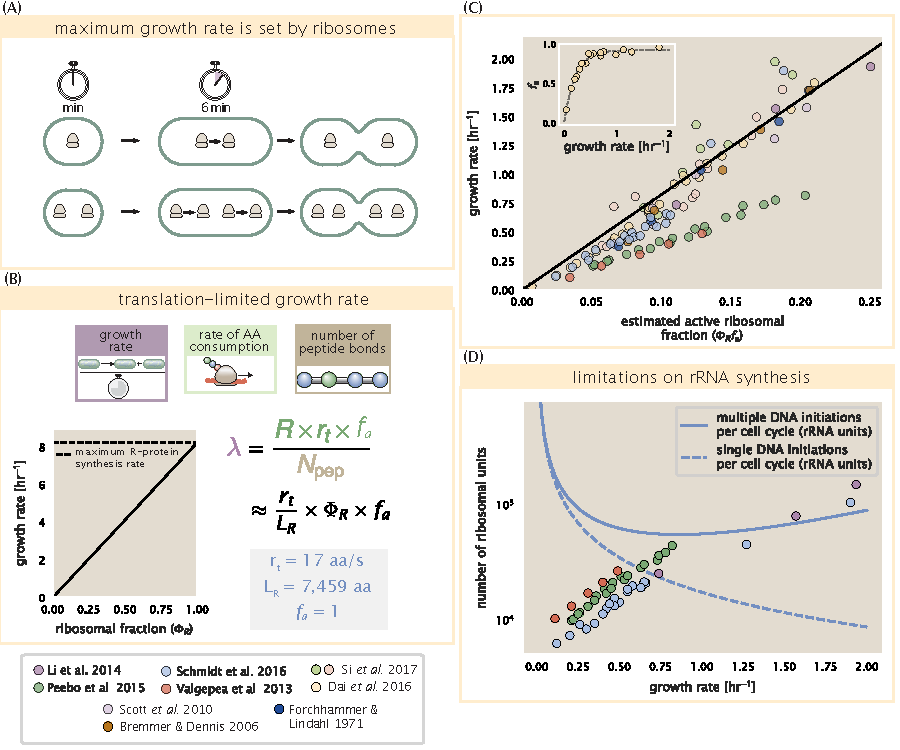
\includegraphics{main_figs/fig7_ribosome_as_limit.pdf}
        \caption{\textbf{Translation-limited growth rate.}  (A) \textit{top}:
        Translation-limited growth as a function of the ribosomal fraction. The
        solid line is calculated for an elongation rate of 17 aa per second.
        The dashed line corresponds to the maximum rate of ribosomal protein
        (R-protein) synthesis considered in part (C).
        \textit{bottom}: Actively translating ribosomal fraction versus growth rate.
        The actively translating ribosomal fraction is calculated using the
        estimated values of $f_a$ from  \cite{dai2016} (shown in inset; see
        Appendix \nameref{sec:SI_f_a} for additional detail). Gray data points
        show additional measurements from literature and consider further in
        \FIGSUPP[ribosome_limit]{ribosome_limit_supp}(A).
        (B) An inherent
        maximum growth rate is set by the time to synthesize all ribosomal
        subunits. This growth rate is given by $r_t/ L_R$, where $r_t$ is
        the elongation rate and $L_R$ is the total number of amino acids
        that make up the entire ribosomal complex. This rate is independent
        of the number of ribosomes and instead is limited by the time required to
        double an individual ribosome.
        (C) Maximum number of
        rRNA units that can be synthesized as a function of growth rate.
        Solid curve corresponding to the rRNA copy number is calculated by
        multipyling the number of rRNA operons by the estimated number of
        $\langle\text{\# ori}\rangle$ at each growth rate. The quantity
        $\langle\text{\# ori}\rangle$ was calculated using Equation 4 and
        the measurements from \cite{si2017} that are plotted in
        \FIG{translation_ecoli_partA}(A). The dashed line shows the maximal
        number of functional rRNA units produced from a single chromosomal
        initiation per cell cycle. }
        \label{fig:ribosome_limit}


        \figsupp[Comparison of $\Phi_R f_a$ with literature and estimation of $\langle$\# ori$\rangle$.]{(A) Actively translating ribosomal fraction versus growth rate.
        The actively translating ribosomal fraction is calculated using the
        estimated values of $f_a$ from  \cite{dai2016} (shown in inset; see
        Appendix \nameref{sec:SI_f_a} for additional detail). Additional measurements
        in addition to the proteomic measurements are based on measurements of cellular RNA to
        protein ratio, with $\Phi_R \approx$ the cellular RNA to
        protein ratio divided by 2.1 \citep{dai2016}. (B) Experimental measurements of
        the cell doubling time $\tau$ and cell cycle time $t_{cyc}$
         from Si \textit{et al.}
        (2017). Dashed line shows fit to the data, which were used to estimate
        $\langle$\# ori$\rangle$. $t_{cyc}$ was assumed to vary in proportion to
        $\tau$ for doubling times greater than 40 minutes, and reach a
        minimum value of 73 minutes. See Appendix
        \nameref{sec:SI_ori} for additional details exact estimation of rRNA copy number. Red data points correspond
        to measurements in strain MG1655, while light green points are for
        strain NCM3722.
        Schematic shows the expected increase in replication forks (or number of
        ori regions) as \textit{E. coli} cells grow faster. }{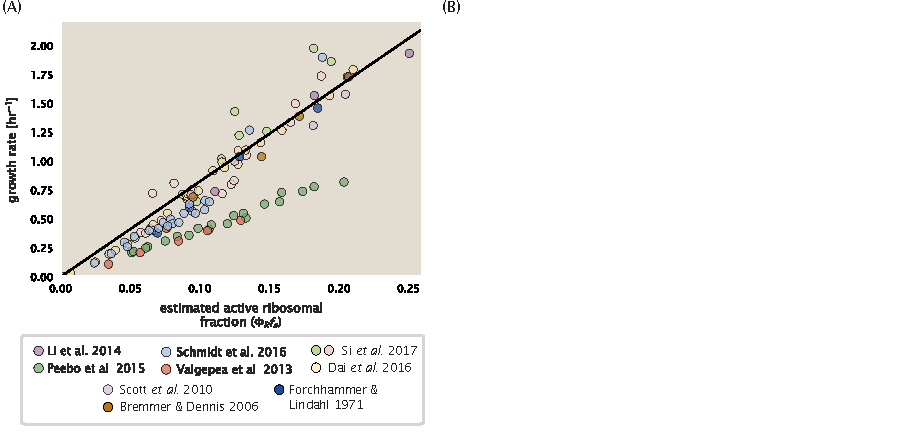
\includegraphics{main_figs/fig7_ribosome_as_limit_Supp.pdf}}\label{figsupp:ribosome_limit_supp}
        }
  \end{fullwidth}
\end{figure}

\subsection{rRNA Synthesis Presents a Potential Bottleneck during Rapid Growth}
\textit{E. coli} rarely exhibits growth rates above 2 hr$^{-1}$
\citep{bremer2008}, which is still well-below the synthesis rate of a single
ribosome, and below the growth rates reported for several other bacteria
\citep{roller2016}. Here we need to also consider ribosomal synthesis from the
perspective of limiting rRNA synthesis, which as we have found earlier, will depend on the
number of rRNA operons to transcribe rRNA.

Due to multiple rounds of chromosomal replication per cell doubling, the
effective number of rRNA operons increases with growth rate and will vary in
proportion to the average number of origins per cell, $\langle$\# ori$\rangle$.
This parameter is set by how often replication must be initiated per cell
doubling in order to maintain steady state growth, and quantified by
\begin{equation}
    \langle \text{\# ori} \rangle = 2^{\tau_{cyc} / \tau} = 2^{\tau_{cyc} \lambda / ln(2)}.
    \label{eq:Nori}
\end{equation}
Here, $t_{cyc}$ is the cell cycle time (referring to the time from replication
initiation to cell division), and $\tau$ is the cell doubling time.  We used the
experimental measurements of $\tau_{cyc}$ and  $\tau$ from \cite{si2017}
(\FIGSUPP[ribosome_limit]{ribosome_limit_supp}(B)) to calculate $\langle$\#
ori$\rangle$  with \EQ{Nori} as a function of growth rates. For growth rates
above about 0.5 hr$^{-1}$, $t_{cyc}$ is approximately constant at about 70
minutes, which means that $\langle$\# ori$\rangle$ will grow exponentially with
growth rate. Since the rRNA operons are predominantly located near to origin of
replication  (BNID: 100352, \cite{dennis2004}), we make the simplifying
assumption that that the number of rRNA operons  will be directly proportional
to $\langle$\# ori$\rangle$.

Returning to our rule-of-thumb of 1 functional rRNA unit per second per operon,
we estimate the maximum number of ribosomes that could be made as a function of
growth rate (\FIG{ribosome_limit}(C), blue curve). Although we expect this
estimate to drastically overestimate rRNA abundance at slower growth rates
($\lambda < 0.5\, \text{hr}^{-1}$), it provides a useful reference alongside the
proteomic measurements. For growth rates above about 1 hr$^{-1}$, we find that
cells will \textit{need} to transcribe rRNA near their maximal rate. As a counter
example, if \textit{E. coli} did not initiate multiple rounds of replication,
they would be unable to make enough rRNA for the observed number of ribosomes
(dashed blue curve in \FIG{ribosome_limit}(C)). The convergence between the
maximum rRNA production and measured ribosome copy number suggests rRNA
synthesis may begin to present a bottleneck at the fastest growth rates due to
the still-limited copies of rRNA genes.


% It is now well-documented that \textit{E. coli} cells add a constant volume per
% origin of replication, which is robust to a remarkable array of cellular
% perturbations \citep{si2017}.

% To consider
% this  in the context of the proteomic data, we used measurements of $\tau_{cyc}$
% and  $\tau$ from \cite{si2017} (\FIG{translation_ecoli_partA}(A)) to
% calculate $\langle$\# ori$\rangle$  with \EQ{Nori} at different growth
% rates. For ribosomal synthesis, we find an approximately linear correlation
% between ribosome copy number and $\langle$\# ori$\rangle$
% (\FIG{translation_ecoli_partA}(B)).
%
% For a constant cell cycle time, which is observed at growth rates above about
% 0.5 hr$^{-1}$ (\FIG{translation_ecoli_partA}(A), \citep{helmstetter1968}),
% \EQ{Nori} states that $\langle \text{\# ori} \rangle$ will need to increase
% exponentially with the growth rate.

% \subsection{Rapid Growth Requires \textit{E. coli} to Increase Both Cell Size and Ribosomal
Mass Fraction}
In the right-hand side of \FIG{ribosome_limit}(B),  we also find that above about 0.75
hr$^{-1}$, the growth rate is determined solely by the ribosomal mass fraction
$\Phi_R$, since $f_a$ is close to 1, and $r_t$ is near its maximal rate
\citep{dai2016}. While $\Phi_R$ will need to increase in order for cells to
grow faster, the fractional dependence in \EQ{lam_limited}
gives little insight into how this scaling is actually achieved by the cell.

It is now well-documented that \textit{E. coli} cells add a constant volume per
origin of replication, which is robust to a remarkable array of cellular
perturbations \citep{si2017}. Given the proteomic measurements featured in this
work, we find that the ribosome copy number also scales in proportion to
$\langle$\# ori$\rangle$ (\FIG{translation_ecoli_partA}(A)). However,  an
increase in ribosome abundance alone is not necessarily sufficient to increase
growth rate and  we also need to consider how $\Phi_R$ varies with $\langle$\#
ori$\rangle$. Importantly, as shown in \FIG{translation_ecoli_partA}(B), we find
that the deviations in protein expression with $\langle$\# ori$\rangle$ are
largely restricted to regions of ribosomal protein genes
\FIG{translation_ecoli_partA}(B). Here we have calculated the position-dependent
protein expression across the chromosome by a running Gaussian average of
protein copy number (20 kbp st. dev. averaging window) based on each gene's
transcriptional start site. These were median-subtracted to account for the
change in total protein abundance with $\langle$\# ori$\rangle$. This result
suggests that $\Phi_R$ is also being tuned in proportion to $\langle$\#
ori$\rangle$ under nutrient-limited growth, and in particular, it is through
this additional dependence on $\Phi_R$, combined with the exponential increase
in $\langle$\# ori$\rangle$, that \textit{E. coli} exhibits an exponential
increase in cell size with growth rate.

% To understand how this relates to growth rate, we
% neeed to consider the changes in proteome composition and ribosome abundance
% with $\langle$\# ori$\rangle$. In \FIG{translation_ecoli_partA}(D),


% For a
% constant cell cycle time $\tau_{cyc}$, which is observed at growth rates above
% about 0.5 hr$^{-1}$ (\FIG{translation_ecoli_partA}(A), \citep{helmstetter1968}),
% \EQ{Nori} states that $\langle \text{\# ori} \rangle$ will need to increase
% exponentially with the growth rate.

%
%
%
% While this says nothing of the observed scaling between cell
% size and growth rate, the additional dependency on ribosomal fraction through
% \EQ{translation_limit_growth_rate} provides an important link.
%
%



%
% To better explore how cells vary protein abundance proteome-wide
% across growth conditions, in \FIG{translation_ecoli_partA}(D), we show that the major deviations
% in protein expression across the chromosome in different growth conditions is a change
% in ribosomal expression.
%
% determined the position-dependent protein expression across the chromosome by
% calculating a running Gaussian average of protein copy number (20 kbp st. dev.
% averaging window) based on each gene's transcriptional start site. These were
% median-subtracted to account for the differences in total protein abundance.
%

%
%
% \subsection{Rapid Growth Requires an Increase in Ribosomal Copy Number and Cell Size}
% In \FIG{ribosome_limit}(C) we find that above about 0.75 hr$^{-1}$, the growth
% rate is dictated by the ribosomal mass fraction $\Phi_R$, since $f_a$ is close
% to 1, and $r_t$ is near its maximal rate [cite and refer to figure/
% supplemental]. While the preceeding section helps us understand that cells will
% need to increase $\Phi_R$ in order to grow faster, the fractional dependence
% gives little insight into how this is actually achieved within the cell. Here we
% consider how the observed changes in absolute protein content
% relate to this dependence between growth rate and $\Phi_R$.
%
% It is now well-documented that \textit{E. coli} cells add a constant volume per
% origin of replication, which is robust to a remarkable array of cellular
% perturbations \citep{si2017}.  The average number of origins per cell, $\langle$\#
% ori$\rangle$, is set by how often replication must be initiated per cell doubling
% under steady state growth. This can be quantified as
% \begin{equation}
%     \langle \text{\# ori} \rangle = 2^{\tau_{cyc} / \tau} = 2^{\tau_{cyc} \lambda / ln(2)},
%     \label{eq:Nori}
% \end{equation}
% where $t_{cyc}$ is the cell cycle time (referring to the time from replication
% initiation to cell division), and $\tau$ is the cell doubling time. To consider
% this  in the context of the proteomic data, we used measurements of $\tau_{cyc}$
% and  $\tau$ from \cite{si2017} (\FIG{translation_ecoli_partA}(A)) to
% calculate $\langle$\# ori$\rangle$  with \EQ{Nori} at different growth
% rates. For ribosomal synthesis, we find an approximately linear correlation
% between ribosome copy number and $\langle$\# ori$\rangle$
% (\FIG{translation_ecoli_partA}(B)).
%
% For a constant cell cycle time, which is observed at growth rates above about
% 0.5 hr$^{-1}$ (\FIG{translation_ecoli_partA}(A), \citep{helmstetter1968}),
% \EQ{Nori} states that $\langle \text{\# ori} \rangle$ will need to increase
% exponentially with the growth rate. While this says nothing of the observed
% scaling between cell size and growth rate, the additional dependency on
% ribosomal fraction through \EQ{translation_limit_growth_rate} provides an
% important link. To better explore how cells vary protein abundance proteome-wide
% across growth conditions, in \FIG{translation_ecoli_partA}(D), we
% determined the position-dependent protein expression across the chromosome by
% calculating a running Gaussian average of protein copy number (20 kbp st. dev.
% averaging window) based on each gene's transcriptional start site. These were
% median-subtracted to account for the differences in total protein abundance.
% Importantly, the major deviations in protein copy number are largely restricted to
% regions of ribosomal protein genes. This suggests that the ribosomal fraction
% $\Phi_R$ is also being tuned in proportion to $\langle$\# ori$\rangle$, and that
% it is through this dependence that \textit{E. coli} exhibits an exponential
% increase in cell volume with growth rate.




\begin{figure*}
    \begin{fullwidth}
    \centering{
        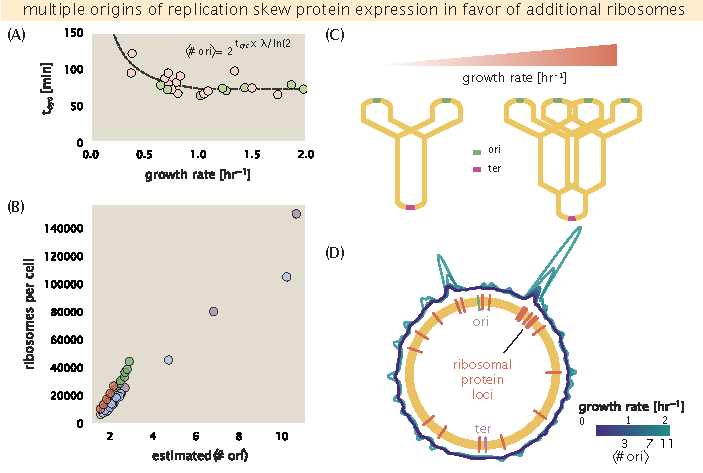
\includegraphics{main_figs/fig8_ribosome_growth_limit_ecoli_a_polar_coord.pdf}
        \caption{\textbf{Cells increase both absolute ribosome abundance and $\Phi_R$ with
        $\langle$\# ori$\rangle$.} (A) Plot of the ribosome copy number estimated from the
        proteomic data against the estimated $\langle$\# ori$\rangle$ (see Appendix
        \nameref{sec:SI_ori} for additional details). (B) A running
        Gaussian average (20 kbp st. dev.) of protein copy number is calculated
        for each growth condition considered by \citep{schmidt2016} based
        on each gene's transcriptional start site. Since total
        protein abundance increases with growth rate, protein copy numbers are
        median-subtracted to allow comparison between growth conditions.
        $\langle$\# ori$\rangle$ are estimated using the data in (A) and
        Equation \ref{eq:Nori}. } \label{fig:translation_ecoli_partA}
    }
    \end{fullwidth}
\end{figure*}

% 
\subsection{Alarmone-Mediated Regulation Controls the Rate of Protein Synthesis}

As we have seen, cell size, total proteomic content, and the number of ribosomes
are all interconnected and influence the achievable growth rate. The drastic
change in these parameters across different growth conditions suggests that
they are being tuned to better match the cell's biosynthetic capacity to the
specific environment. Take, as another illustration of this, the recent
experimental work by \cite{dai2016}. In one set of experiments the authors
considered growth in cells whose primary glucose transport system was disrupted
($\Delta$\textit{ptsG}). Unsurprisingly, the growth rate was reduced, and was
measured at about two-fold slower than their wild-type line.  This change,
however, was not simply the result of now-limiting carbon uptake. Instead, cells
accomodated the perturbation by also reducing their ribosomal mass fraction by
a factor of two, which is still in line with \EQ{translation_limit_growth_rate}
under translation-limited growth.  In this final, we explore the interconnection
between cell size, ribosome content, and growth rate by formulating a minimal
model of growth rate control. We use it to quantitatively show how tuning these
parameters help cells maximize their growth rate.

To react to changes in nutrient conditions, bacteria rely on the synthesis or
degradation of secondary-messenger molecules  like (p)ppGpp, which cause global
changes in transcriptional and translational activity. In \textit{E. coli},
amino acid starvation causes the accumulation of de-acylated tRNAs at the
ribosome's A-site and leads to a strong increase in (p)ppGpp synthesis activity
by the enzyme RelA \citep{hauryliuk2015}. Cells also accumulate (p)ppGpp  during
steady-state growth in poorer growth conditions, which leads to a decrease in
the fraction of actively translating ribosomes, $f_a$  (with $f_a \approx 0.5$
at a growth rate of $\approx$ 0.3 hr$^{-1}$; \FIG{ribosome_limit}(C) - inset).

Furthermore, (p)ppGpp can inhibit the initiation of DNA replication by mediating
a change in transcriptional activity and the supercoiling state of the origin of
replication \citep{kraemer2019}. These observations all raise the possibility
that it is through (p)ppGpp that cells mediate the growth-rate dependent changes
in $\langle$\# ori$\rangle$, cell size, and ribosomal abundance and activity
\citep{zhu2019, Buke2020}. Indeed, recent work in a (p)ppGpp deficient strain of
\textit{E. coli} found that cells exhibited a high ratio of $\langle$\#
ori$\rangle$ to $\langle$\# ter$\rangle$, and cell sizes that were more
consistent with a fast growth state where (p)ppGpp levels are normally low
\citep{fernandezcoll2020}.

\subsection{Ribosomal Elongation Rate and Cellular Growth Rate are Linked by
Amino Acid Scarcity}
Here we consider a mode of regulation in which the rate of peptide elongation
$r_t$ depends only on the availability of amino acids (and, therefore, also
amino-acyl tRNAs). It is through the elongation rate $r_t$ that we assume cells
adjust their ribosomal content ($R$, $\Phi_R$) according to nutrient
availability and for simplicity, do not explicitly model changes in  $\langle$\#
ori$\rangle$ or regulation by (p)ppGpp.

The rate of elongation $r_t$ will depend on how quickly the ribosomes can match
codons with their correct amino-acyl tRNA, along with the subsequent steps of
peptide bond formation and translocation. We therefore coarse-grain the steps of
elongation to two time-scales,  1) the time required to find and bind each
correct amino-acyl tRNA, and 2) the remaining steps in peptide elongation that
will not depend on the amino acid availability. Under this model, other
molecular players required for translation like elongation factors and GTP are
considered in sufficient abundance, which appear to be valid assumptions given
our analysis of the proteomic data and energy production thus far. The time to
translate each codon is given by the inverse of the elongation rate $r_t$, which
can be written as,

\begin{equation}
\frac{1}{r_t} = \frac{1}{k_{on} \alpha [AA]_{\text{eff}}} + \frac{1}{r_{t}^{\text{max}}}.
\end{equation}
where we have assumed that the rate of binding by amino-acyl tRNA $k_{on}$ is
proportional to $[AA]_{\text{eff}}$ by a constant $\alpha$. The second term on
the right-hand side reflects our assumption that other steps in peptide
elongation are not rate-limiting, with a maximum elongation rate
$r_{t}^{\text{max}}$ of about 17 amino acids per second \cite{dai2016}. As the
rate of amino acid supply, denote by $r_{AA}$, varies with changing nutrient
condtions, the cell can maximize the rate of protein synthesis by tuning the
rate of amino acid consumption (mathematized as $r_t \times R \times f_a$) ,
shown schematically in \FIG{elongation_rate_model}(A). This can be stated more
succinctly in terms of an effective dissociation constant, $K_D = r_{t}^{\text{max}} / \alpha k_\text{on}$, where the elongation rate $r_t$ is now given by

\begin{equation}
r_t = \frac{r_{t}^{\text{max}}}{1 + K_D/[AA]_{\text{eff}}}.
\label{eq:rt_kd_simple}
\end{equation}

Under steady-state growth, the amino acid concentration is constant
($\frac{d[AA]_\text{eff}}{dt}=0$) and will relate to the rate of amino acid
synthesis (or import, for rich media) and/or tRNA charging, as $r_{AA}$, and the
rate of consumption, $r_t\times R \times f_a$ by,

\begin{equation}
\int_{0}^{t} \frac{d[AA]_{\text{eff}}}{dt} dt =  \int_{0}^{t}([r_{AA}] - [r_t\times R \times f_a]) dt,
\label{eq:aaeff_int}
\end{equation}
where the time from 0 to $t$ is an arbitrary length of time, and the square
brackets indicate concentrations per unit time. Integrating \EQ{aaeff_int}
yields,

\begin{equation}
   [AA]_\text{eff} = \frac{t(r_{AA} - r_t \times R \times f_a)}{V},
   \label{eq:aa_final}
\end{equation}
with  $r_{AA}$ is in units of AA per unit time and $r_t$ is in units of AA per
unit time per ribosome, for a cell with average volume $V$. Plugging \EQ{aa_final}
into \EQ{rt_kd_simple} allows us to then solve for $r_t$ and
a complete derivation is provided in Appendix \ref{sec:SI_model}.

In \FIG{elongation_rate_model}(B), we illustrate how the elongation rate depends
on the ribosomal copy number. Here, we have considered a unit volume $V =
1$\textmu m$^3$, a unit time $t = 1$ s, a $K_D = 5$ mM (inferred from
\cite{bennett2009}), $f_a = 1$, and an arbitrarily chosen $r_{AA} = 5\times 10^6$ AA
$\cdot$ s$^{-1} \cdot$ \textmu m$^{-3}$. At low ribosome copy numbers, the
observed elongation rate is dependent primarily on the ratio of $K_D / Vr_{AA}$
[as $r_t^{\text{max}} \times R \times f_a << r_{AA}$, point (1) in
\FIG{elongation_rate_model}(B)]. As the ribosome copy number is increased such
that the amino acid supply rate and  consumption rate are nearly equal [point
(2) in \FIG{elongation_rate_model}(B)], the observed elongation rate begins to
decrease sharply. When the ribosome copy number is increased even further,
consumption at the maximum elongation rate exceeds the supply rate, yielding  a
significantly reduced elongation rate [point (3) in
\FIG{elongation_rate_model}{B)]. While the elongation rate will always be
dominated by the amino acid supply rate at sufficiently low ribosome copy
numbers, the elongation rate at larger ribosome abundances can be increased by
tuning $f_a$ such that not all ribosomes are elongating, reducing the total
consumption rate.

\begin{figure}
    \centering{
        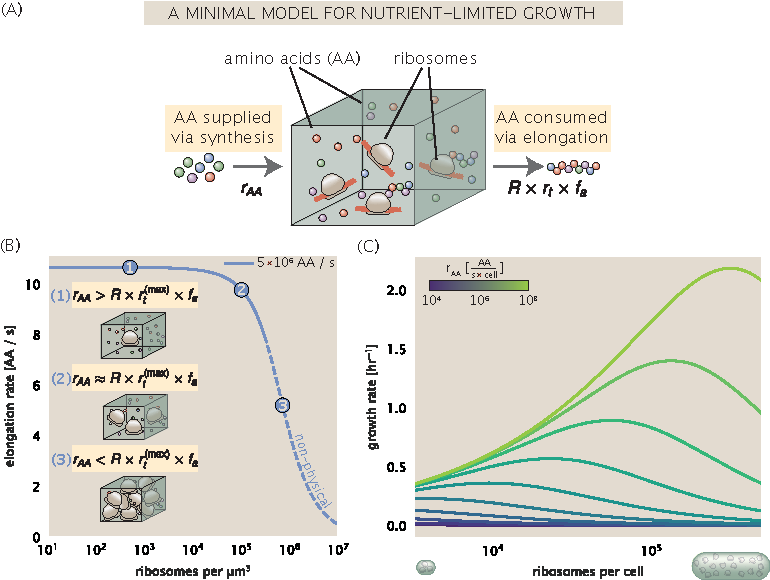
\includegraphics{main_figs/elongation_model.pdf}
        \caption{\textbf{A minimal model of growth rate control under
        nutrient limitation.} (A) We consider a unit volume of cellular material
        composed of amino acids (colored spheres) provided at a supply rate
        $r_{AA}$. These amino acids are polymerized by a pool of ribosomes
        (brown blobs) at a rate $r_t \times R \times f_a$, where $r_t$ is the
        elongation rate, $R$ is the ribosome copy number in the unit volume, and
        $f_a$ is the fraction of those ribosomes actively translating. (B) The
        observed elongation rate is plotted as a function of ribosomes in a unit
        volume \textmu m$^3$. The three points correspond to three regimes of
        ribosome copy numbers and are shown schematically on the left-hand side.
        The region of the curve shown as dashed lines represents a non-physical
        copy number, but is shown for illustrative purposes. This curve was
        generated using the parameters $r_{AA} = 5 \times 10^6$ AA / s, $K_D =
        5$ mM, and $r_t^\text{(max)} = 17.1$ AA / s. (C) The cellular growth
        rate is plotted as a function of total cellular ribosome copy number for
        different cellular amino acid supply rates, with blue and green curves
        corresponding to low and high supply rates, repsectively. As the
        ribosome copy number is increased, so too is the cell volume and total
        protein abundance. We direct the reader to the Suppemental Information
        for discussion  on the inference of the realtionship between cell
        volume, number of peptide bonds, and ribosome copy number.}
        \label{fig:elongation_rate_model}
    }
\end{figure}

\subsubsection{Optimal Growth Rate, Ribosomal Content, and Cell Size Depend on Nutrient
Availability and Metabolic Capacity.}

To relate elongation rate to growth rate, we constrain the set of parameters
based on our available proteomic measurements; namely, we restrict the values of
$R$, $N_{pep}$, and $V$ to those associated with the amalgamated proteomic data
(described in Appendix \nameref{estimate_protein_per_cell}). We then consider
how changes in the nutrient conditions, through the parameter $r_{AA}$,
influence the maximum growth rate as determined by \EQ{lambda_limit}.
\FIG{elongation_rate_model}(C) shows how the observed growth rate depends on the
rate of amino acid supply $r_{AA}$ as a function of the cellular ribosome copy
number. A feature immediately apparent is the presence of a maximal growth rate
whose dependence on $R$ (and consequently, the cell size) increases with
increasing $r_{AA}$. Importantly, however, there is an optimum set of $R$,
$N_{pep}$, and $V$ that are strictly dependent on the value of $r_{AA}$.
Increasing the ribosomal concentration beyond the cell's metabolic capacity has
the adverse consequence of depleting the supply of amino acids and a concomitant
decrease in the elongation rate $r_t$ [\FIG{elongation_rate_model}(B)].

Also of note is the growth rate profiles shown for low amino acid supply rates
[purple and blue lines in \FIG{elongation_rate_model}(C)], representing growth
in nutrient-poor media. In these conditions, there no longer exists a peak in
growth, at least in the range of physiologically-relevant  ribosome copy
numbers. Instead, cells limit their pool of actively translating ribosomes  by
decreasing $f_a$ \citep{dai2016}, which would help maintain the pool of
available amino acids $[AA]_\text{eff}$ and increase the achievable elongation
rate. This observation is in agreement with the central premise of the cellular
resource allocation principle proposed by \cite{scott2010,
klumpp2009,klumpp2014} and \cite{hui2015}.

\section{Discussion}
Continued experimental and technological improvements have led to a treasure
trove of quantitative biological data \citep{hui2015, schmidt2016, si2017,
gallagher2020, peebo2015, valgepea2013}, and an ever advancing molecular view
and mechanistic understanding of the constituents that support bacterial
growth \citep{taheriaraghi2015, morgenstein2015, si2019, karr2012,
kostinski2020, macklin2020}. In this work we have compiled what we believe to be the
state-of-the-art knowledge on proteomic copy number across a broad range of
growth conditions in \textit{E. coli}. We have made this data accessible
through a \href{https://github.com/RPGroup-PBoC/growth_limits}{GitHub
repository}, and an \href{https://rpgroup.caltech.edu/growth_limits//data_explorer}{interactive
figure} that allows exploration of specific
protein and protein complex copy numbers. Through a series of
order-of-magnitude estimates that traverse key steps in the bacterial cell
cycle, this proteomic data has been a resource to guide our understanding of
two key questions: what biological processes limit the absolute speed limit
of bacterial growth, and how do cells alter their molecular constituents as a
function of changes in growth rate or nutrient availability? While not
exhaustive, our series of estimates provide insight on the scales of
macromolecular complex abundance across four classes of cellular processes --
the transport of nutrients, the production of energy, the synthesis of the
membrane and cell wall, and the numerous steps of the central dogma.

In general, the copy numbers of the complexes involved in these processes were
in reasonable agreement with our order-of-magnitude estimates. Since many of these
estimates represent soft lower-bound quantities, this suggests that cells do not
express proteins grossly in excess of what is needed for a particular growth
rate. Several exceptions, however, also highlight the dichotomy between a
proteome that appears to "optimize" expression according to growth rate and one
that must be able to quickly adapt to environments of different nutritional
quality. Take, for example, the expression of carbon transporters. Shown in
\FIG{carbon_tport}(B), we find that cells always express a similar number of
glucose transporters irrespective of growth condition. At the same time, it is
interesting to note that many of the alternative carbon transporters are still
expressed in low but non-zero numbers ($\approx$ 10-100 copies per cell) across
growth conditions. This may relate to the regulatory configuration for many of
these operons, which require the presence of a metabolite signal in order for
alternative carbon utilization operons to be induced \citep{monod1949,
laxhuber2020}. Furthermore, upon induction, these transporters are expressed and
present in abundances in close agreement with a simple estimate.

Of the processes illustrated in \FIG{categories}, we arrive at a
ribosome-centric view of cellular growth rate control. This is in some sense
unsurprising given the long-held observation that \textit{E. coli} and many
other organisms vary their ribosomal abundance as a function of growth
conditions and growth rate \citep{scott2010, metzlraz2017}. However, through our
dialogue with the proteomic data, two additional key points emerge. The first
relates to our question of what process sets the absolute speed limit of
bacterial growth. While a cell can parallelize many of its processes simply by
increasing the abundance of specific proteins or firing multiple rounds of DNA
replication, this is not so for synthesis of ribosomes
[\FIG{ribosome_limit}(A)]. The translation time for each ribosome [$\approx$ 7
min, \cite{dill2011}] places an inherent limit on the growth rate that can only
be surpassed if the cell were to increase their polypeptide elongation rate, or
if they could reduce the total protein and rRNA mass of the ribosome. The second
point relates to the long-observed correlations between growth rate and cell
size \citep{schaechter1958, si2017}, and between growth rate and ribosomal mass
fraction. While both trends have sparked tremendous curiosity and driven
substantial amounts of research in their own regards, these relationships are
themselves intertwined. In particular, it is the need for cells to increase
their absolute number of ribosomes under conditions of rapid growth that require
cells to also grow in size. Further experiments are needed to test the validity
of this hypothesis. In particular, we believe that the change in growth rate in
response to translation-inhibitory drugs (such as chloramphenicol) could be
quantitatively predicted, given one had precision measurement of the relevant
parameters, including the fraction of actively translating ribosomes $f_a$ and
changes in the metabolic capacity of the cell (i.e. the rate that amino acids can be made
available) for a particular growth condition.

While the generation of new ribosomes plays a dominant role in growth rate
control, there exist other physical limits to the function of cellular
processes. One of the key motivations for considering energy production was the
physical constraints on total volume and surface area as cells vary their size
\citep{harris2018, ojkic2019}. As \textit{E. coli} get larger at faster growth
rates, an additional constraint begins to arise in energy production and
nutrient uptake due to the relative decrease in total surface area, where ATP is
predominantly produced \citep{szenk2017}. Specifically, the cell interior
requires an amount of energy that scales cubically with cell size, but the
available surface area only grows quadratically [\FIG{energy_scaling}(A)]. While
this threshold does not appear to be met for \textit{E. coli} cells growing at 2
hr$^{-1}$ or less, it highlights an additional constraint on growth given the
apparent need to increase cell size in order to grow faster. This limit is
relevant even to eukaryotic organisms, whose mitochondria exhibit convoluted
membrane structures that nevertheless remain bacteria-sized organelles
\citep{guo2018}. In the context of bacterial growth and energy production more
generally, we have mainly limited our analysis to the aerobic growth conditions
associated with the proteomic data and further consideration will be needed for
anaerobic growth.1

This work is by no means meant to be a complete dissection of bacterial
growth rate control, and there are many aspects of the bacterial proteome and
growth that we neglected to consider. For example, other recent work
\citep{liebermeister2014, hui2015, schmidt2016} has explored how the proteome is
structured and how that structure depends on growth rate. In the work of
\cite{hui2015}, the authors coarse-grained the proteome into six discrete
categories being related to either translation, catabolism, anabolism, and
others related to signaling and core metabolism. The relative mass fraction of
the proteome occupied by each sector could be modulated by external application
of drugs or simply by changing the nutritional content of the medium. While we
have explored how the quantities of individual complexes are related to cell
growth, we acknowledge that higher-order interactions between groups of
complexes or metabolic networks at a systems-level may reveal additional
insights into how these growth-rate dependences  are mechanistically achieved.
Furthermore, while we anticipate the conclusions summarized here are applicable
to a wide collection of bacteria with similar lifestyles as \textit{E. coli},
other bacteria and archaea may have evolved other strategies that were not
considered. Further experiments with the level of rigor now possible in
\textit{E. coli} will need to be performed in a variety of microbial organisms
to learn more about how regulation of proteomic composition and  growth rate
control has evolved over the past 3.5 billion years.

%
%
%
%
% our estimates are
% appear to be in excess of what would be minimally required to support cell
% growth at the observed rates.
%
%
%  to elucidate a
% fundamental question in bacterial physiology -- what sets the speed limit at
% which cells can divide?


%
% Recent years have seen an explosion in our understanding of the cellular
% macromolecular composition at unprecedented resolution. This quantitative,
% molecular view of cell biology has transformed our understanding of how and when
% genes are expressed, to what degree they are expressed, and precisely how they
% are post-translationally modified (a topic we have not considered in this work,
% but appreciate nonetheless). Despite these impressive studies, an understanding
% of how the abundance and regulation is related to growth rate has been largely
% treated with phenomenological models, often containing obscure dimensionless
% parameters or polynomial fits to data. While these phenomenological treatments
% have revealed fascinating features of the resource allocation within the
% proteome, elucidating the molecular details of \textit{how} these resource
% allocation strategies operate has remained enigmatic.
%
% In this work, we present a series of order-of-magnitude estimates to elucidate a
% fundamental question in bacterial physiology -- what sets the speed limit at
% which cells can divide?
%
%
% Countless careers have been built examining the minutiae of each of
% the processes listed in \FIG{categories}, resulting in a treasure
% trove of literature representing decades of careful experimentation, modeling,
% and interpretation of results. Despite the undeniable complexity of each
% individual process, our work illustrates that in order to understand what sets
% the scale of the observed protein copy numbers and their corresponding
% dependence on growth rate, a coarse-grained view of the system is often
% appropriate.
%
%
% [GC: Other topics to discuss include the utility of scrounging the data from the
% literature to assemble, to our knowledge, the most complete view of the
% condition-dependent proteome of \textit{E. coli}.]
%
%
% [Fill in.]

% Parallelized DNA replication represents a solution that allows  \textit{E. coli}
% to synthesize enough rRNA as it grows faster. That the cell appears to
% be synthesizing rRNA near its maximal rate at growth rates above about 0.5 h$^{-1}$
% may also have consequences on robust scaling  between
% cell size and $\langle$\# ori$\rangle$. As one example, when cells are exposed
% to sublethal doses of ribosome-inhibiting drugs like chloramphenicol, there is a
% notable increase in the cell's ribosomal fraction (grey points,
% \FIG{translation_ecoli_partA}(D)), but otherwise the cell is able to maintain
% its cell size according to $\langle$\# ori$\rangle$ \citep{si2017}. While the
% presence of chloramphenicol will inhibit protein synthesis, it will also allow
% for relatively higher rRNA synthesis due to the longer doubling time. If the
% cell can scale it ribosomal protein abundance through feedback from rRNA
% synthesis, than we would expect the relative abundance of ribosomes to increase
% according to the increase in rRNA synthesis. This type of feedback was
% considered long ago \citep{nomura1984} and we consider this possibility further
% in Supplemental Appendix XX.


% While it is difficult to distinguish between causality and correlation, the data
% also helps us resolve why cell size, should exhibit an exponential increase with growth
% rate once cells begin to parallelize DNA replication. Specifically,
%
% is consistent with the need for cells to increase their effective rRNA gene
% dosage in order to grow according to the constraint set by Equation 2. Importantly, it
% may also shed some light on the notable increase in ribosomal content
% that is observed when sublethal doses of antibiotics \citep{scott2010, dai2016}.
% Specifically, if rRNA synthesis is rate limiting, and nutrient conditions
% largely dictate the extent of overlapping DNA replication cycles, than addition
% of antibiotic will lengthen the doubling time and allow increased rRNA
% synthesis relative to the rate of cell division. In Supplemental Section XX, we
% consider this further using additional data from \cite{si2017}.


% A number of recent papers further highlight the possibility that regulation
% (p)ppGpp may be the critical component of the apparent scaling laws in
% \textit{E. coli}. In the context of ribosomal activity, increased levels of
% (p)ppGpp are associated with lower ribsomal content, and at slow growth
% are associated with reduced activity by ribosomes and RNA polymerse \citep{dai2016,
% dai2018} [citations for RNAP]. Titration of the cellular (p)ppGpp concetrations (up or down) can
% invoke similar proteomic changes reminiscent of those observed under nutrient
% limitation \citep{zhu2019}. In light of the limiting dependence of ribosome copy
% number on chromosomal gene dosage, it was recently shown that growth in a
% (p)ppGpp null strain abolishes both the scaling in cell size  and the
% $\langle$\# ori$\rangle$ / $\langle$\# ter$\rangle$ ratio. Instead, cells
% exhibited a high $\langle$\# ori$\rangle$ / $\langle$\# ter$\rangle$ closer to 4
% and cell size more consistent with a fast growth state where (p)ppGpp levels are
% low \citep{fernandezcoll2020}. From these results, perhaps the perspective to
% take is that the scaling laws  reflect an attempt for the cell to mitigate its
% biological activity according  to available nutrients.



%%%%%%%%%%%%%%%%%%%%%%%%%%%%%%%%%%%%%%%%%%%%%%%%%%%%%%%%%%%%
%%% Appendix START
%%%%%%%%%%%%%%%%%%%%%%%%%%%%%%%%%%%%%%%%%%%%%%%%%%%%%%%%%%%%
\newpage


\title{Supplemental material for: Fundamental limits on the rate of bacterial cell division}
% \author[1, $\dagger$]{Nathan M. Belliveau}
% \author[2, $\dagger$]{Griffin Chure}
% \author[3]{Christina L. Hueschen}
% \author[4]{Hernan G. Garcia}
% \author[5]{Jane Kondev}
% \author[6]{Daniel S. Fisher}
% \author[1, 7, *]{Julie A. Theriot}
% \author[8, 9, *]{Rob Phillips}
% \affil[1]{Department of Biology, University of Washington, Seattle, WA, USA}
% \affil[2]{Department of Applied Physics, California Institute of Technology, Pasadena, CA, USA}
% \affil[3]{Department of Chemical Engineering, Stanford University, Stanford, CA, USA}
% \affil[4]{Department of Molecular Cell Biology and Department of Physics, University of California Berkeley, Berkeley, CA, USA}
% \affil[5]{Department of Physics, Brandeis University, Waltham, MA, USA}
% \affil[6]{Department of Applied Physics, Stanford University, Stanford, CA, USA}
% \affil[7]{Allen Institute for Cell Science, Seattle, WA, USA}
% \affil[8]{Division of Biology and Biological Engineering, California Institute of Technology, Pasadena, CA, USA}
% \affil[9]{Department of Physics, California Institute of Technology, Pasadena, CA, USA}
% \affil[*]{Co-corresponding authors. Address correspondence to phillips@pboc.caltech.edu and jtheriot@uw.edu}
% \contrib[$\dagger$]{These authors contributed equally to this work}

\maketitle

\newpage
\tableofcontents

\newpage
\section{Experimental Details Behind Proteomic Data}
\label{sec:SI_exp_summary}
Here we provide a brief summary of the experiments behind each proteomic data
set considered. The purpose of this section is to identify how the authors
arrived at absolute protein abundances. In the following section
(see section on~\nameref{sec:SI_data_summary}) we will then provide a summary of the
protein abundance measurements. Table \ref{tab:datasets} provides an overview of
the publications we considered. These are predominately mass spectrometry-based,
with the exception of the work from \cite{li2014} which used ribosomal
profiling, and the fluorescence-based counting done in \cite{taniguchi2010}.
After having compiled and comparing these  measurements, we noted substantial
deviations in the measurements from \cite{taniguchi2010} and \cite{soufi2015}
(shown in the following section), and decided to only use the data from
\cite{taniguchi2010, li2014, valgepea2013, peebo2015} in the main text. For
completeness, we include these additional datasets in our discussion of the experimental
data.

\begin{table}[bt]
\caption{\label{tab:datasets}Overview of proteomic data sets.}
\begin{tabular}{l l l }
\toprule
Author & Method & Reported Quantity \\
\midrule
Taniguchi \textit{et al.} (2010)  & YFP-fusion, cell fluorescence    & fg/copies per cell      \\
Valgepea \textit{et al.} (2012)   & mass spectrometry                & fg/copies per cell      \\
Peebo \textit{et al.} (2014)      & mass spectrometry                & fg/copies per fl        \\
Li \textit{et al.} (2014)         & ribosomal profiling              & fg/copies per cell $^a$ \\
Soufi \textit{et al.} (2015)      & mass spectrometry                & fg/copies per cell      \\
Schmidt \textit{et al.} (2016)    & mass spectrometry                & fg/copies per cell $^b$ \\
\bottomrule
\end{tabular}

\medskip
a. The reported values assume that the proteins are long-lived compared to the
generation time but are unable to account for post-translational modifications
that may alter absolute protein abundances.
\\
b. This mass spectrometry approach differs substantially from the others since
in addition to the relative proteome-wide abundance measurements, the authors
performed absolute quantification of 41 proteins across all growth conditions
(see section on~\nameref{sec:SI_schmidt} for more details on this).
\end{table}

\subsection{Fluorescence based measurements}
In the work of \cite{taniguchi2010}, the authors used a chromosomal YFP fusion
library where individual strains have a specific gene tagged with a YFP-coding
sequence. 1018 of their 1400 attempted strains were used in the work. A
fluorescence microscope was used to collect cellular YFP intensities across  all
these strains. Through automated image analysis, the authors normalized
intensity measurements by cell size to account for the change in size and
expression variability across the cell cycle. Following correction of  YFP
intensities for cellular autofluorescence, final absolute protein levels were
determined by a calibration curve with single-molecule fluorescence intensities.
This calibration  experiment was performed separately using a purified YFP
solution.

\subsection{Ribosomal profiling measurements}
The work of \cite{li2014} takes a sequencing based approach to estimate protein
abundance. Ribosomal profiling, which refers to the deep sequencing of
ribosome-protected mRNA fragments, can provide a quantitative measurement of the
protein synthesis rate.  As long as the protein life-time is long relative to
the cell doubling time, it is possible to  estimate absolute protein copy
numbers. The absolute protein synthesis rate has units of  proteins per generation,
and for stable proteins will also correspond to the protein  copy number per
cell.

In the experiments, ribosome-protected mRNA is extracted from cell lysate  and
selected on a denaturing polyacrylamide gel for deep sequencing (15–45 nt long
fragments collected and sequenced  by using an Illumina HiSeq 2000 in
\cite{li2014}). Counts of ribosome footprints from the sequencing data were then
corrected empirically for position-dependent biases in ribosomal density across
each gene, as well as dependencies on specific sequences including the
Shine-Dalgarno sequence. These data-corrected ribosome densities represent
relative protein synthesis rates. Absolute protein synthesis rates are obtained
by multiplying the relative rates by the total cellular protein per cell. The
total protein  per unit volume  was determined with the Lowry method to quantify
total protein, calibrated against bovine serum albumin (BSA). By counting
colony-forming units following serial dilution of their cell cultures, they then
calculated the total protein per cell.

\subsection{Mass spectrometry measurements}
Perhaps not surprisingly, the data is predominantly mass spectrometry based. This is
largely due to tremendous improvements in the sensitivity of mass spectrometers,
as well as improvements in sample preparation and data analysis
pipelines. It is now a relatively routine task to extract protein from a cell
and quantify the majority of proteins present by shotgun proteomics. In general, this
involves lysing cells, enzymatically digesting the proteins into short peptide
fragments, and then introducing them into the mass spectrometer (e.g.
with liquid chromatography and electrospray ionization), which itself can
have multiple rounds of detection and further fragmentation of the peptides.

Most quantitative experiments rely on labeling protein with stable isotopes,
which allow multiple samples to be measured together by the mass spectrometer.
By measuring samples of known total protein abundance simultaneously (i.e. one
sample of interest, and one reference), it is possible to determine relative
protein abundances. Absolute protein abundances can be estimated following the
same approach used above for ribosomal profiling, which is to multiply each
relative abundance measurement by the total cellular protein per cell. This is
the approach taken by \cite{valgepea2013, peebo2015} and \cite{soufi2015}, with
relative protein abundances determined based on the relative peptide intensities
(label free quantification 'LFQ' intensities). For the data of
\cite{valgepea2013}, total protein per cell was determined by measuring  total
protein by the Lowry method, and counting colony-forming units following serial
dilution. For the data from   \cite{peebo2015}, the authors did not determine
cell quantities and instead report the cellular protein abundances in protein
per unit  volume by assuming a mass density of 1.1 g/ml, with a 30\% dry mass
fraction.

An alternative way to arrive at absolute protein abundances is to dope in
synthetic peptide  fragments of known abundance. These can serve as a direct way
to calibrate mass spectrometry  signal intensities to absolute mass. This is the
approach taken by \cite{schmidt2016}. In addition  to a set of shotgun proteomic
measurements to determine proteome-wide relative abundances,  the authors also
performed absolute quantification of  41 proteins covering over four orders of
magnitude in cellular abundance. Here,  a synthetic peptide was generated for
each of the proteins, doped into each protein sample, and used these to
determine absolute protein abundances of the 41 proteins. These absolute
measurements, determined for every growth condition,  were then used as a
calibration curve to convert proteomic-wide relative abundances into  absolute
protein abundance per cell. A more extensive discussion of the
\cite{schmidt2016} data set can be found in Section \nameref{sec:SI_schmidt}.

\section{Summary of Proteomic Data}
\label{sec:SI_data_summary}
In the work of the main text we only used the data from \cite{valgepea2013,
li2014, peebo2015, schmidt2016}. As shown in \FIG{total_protein_final}(A), the
reported total protein abundances in the work of \cite{taniguchi2010} and
\cite{soufi2015} differed quite substantially from the other work. For the work
of \cite{taniguchi2010} this is in part due to a lower coverage in total
proteomic mass quantified, though we also noticed that most proteins appear
undercounted when compared to the other data.

\FIG{total_protein_final}(B) summarizes the total protein mass for each data
set used in our final compiled data set. Our inclination initally was to
leave reported copy numbers untouched, but a notable descrepency between the scaling
of the total protein per cell between \cite{schmidt2016} and the other data sets
forced us to dig deeper into those measurements (compare \cite{schmidt2016} and
\cite{li2014} data in \FIG{total_protein_final}(A)). The particular trend in
\cite{schmidt2016} appears to be due to assumptions made about cell size and we
provide a more extensive discussion and analysis of their data in
\nameref{sec:SI_schmidt}. As a compromise, and in an effort to treat all data
equally, we instead applied an correction factor to all protein abundance values
based on a data-driven estimate of total protein per cell. Here we used cell
size measurements from \cite{si2017, si2019}, and an estimate of total protein
content through expected dry mass. Total protein per cell was then determined
using available data on total DNA, RNA, and protein from \cite{basan2015,
dai2016}, which  account for the majority of dry mass in the cell. We describe
these details further in sections  on \nameref{sec:protein_size_SV} and
\nameref{sec:estimate_protein_per_cell} that follows.

\begin{figure}
    \begin{fullwidth}
    \centering{
        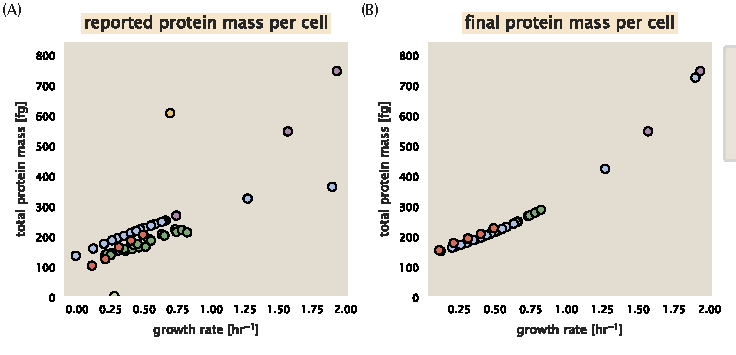
\includegraphics{SI_figs/dataset_corrections.pdf}
        \caption{\textbf{Summary of the growth-rate dependent total protein
        abundance for each data set.} (A) Total protein abundance per cell as
        originally reported in the data sets of \cite{taniguchi2010, valgepea2013, li2014,
        soufi2015, peebo2015, schmidt2016}. Note that the data from \cite{peebo2015} only
        reported protein abundances per unit volume and total protein per cell
        was found by multiplying these by the growth-rate dependent cell size as
        determined by \cite{si2017}. (B) Adjusted total protein abundances
        across the proteomic data sets are summarized. Protein abundances were
        adjusted so that all data shared a common set of growth-rate dependent
        total protein per cell and cellular protein concentration following the
        cell size expectations of \cite{si2017} (see section on
        \nameref{sec:protein_size_SV} for further details). }
        \label{fig:total_protein_final}
    }
    \end{fullwidth}
\end{figure}

Lastly, in \FIG{venn} we show the total proteomic coverage and overlap of
proteins quantified across each data set. In part (A) we plot the total number
of  unique proteins, while in part (B) we plot a Venn diagram to also show the
intersections across each data set. Overall, the overlap in quantified proteins
is quite high, with 1157 proteins quantified across all data sets. The
sequencing based approach of \cite{li2014} has substantially higher coverage
compared to the mass spectrometry data sets (3394 genes versus the 2041 genes
quantified in the work of \cite{schmidt2016}). However, in terms of total
protein mass, the data from \cite{li2014, schmidt2016, peebo2015} each quantify
roughly equivalent total protein mass.  An exception to this is in the data from
\cite{valgepea2013}, where we find that  the total protein quantified in
\cite{valgepea2013} is 90-95 \% of the total protein mass (when using the data
from \cite{schmidt2016} as a reference).


% \begin{figure*}
%     \centering{
%         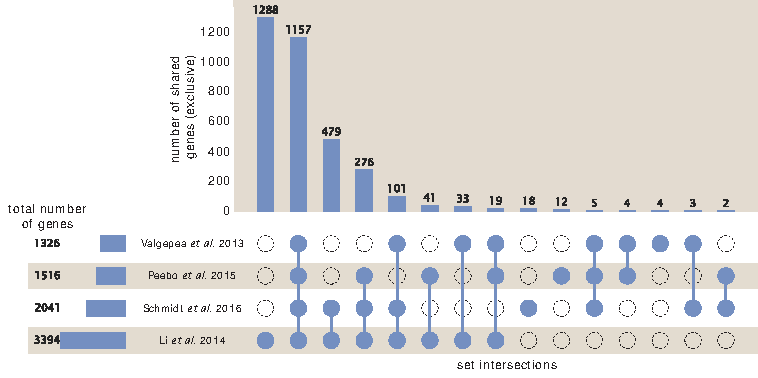
\includegraphics{SI_figs/dataset_upset_diagram.pdf}
%         \caption{\textbf{Comparison of proteomic coverage across different data sets.}
%         An UpSet diagram \citep{Lex2014} summarizes the total number of protein
%         coding genes whose protein abundance was reported in the data sets of
%         \cite{valgepea2013, li2014, schmidt2016, peebo2015}. Bar plot on bottom
%         left indicates the total number of genes reported in each individual
%         data. The main bar plot summarizes the number of unique proteins
%         identified across overlapping subsets of the data.  For example, in the
%         first column only the data from \cite{li2014}  is considered (indicated
%         by solid blue circle) and 1288 proteins are identified as exclusive to
%         the data set. In the second column, the intersection of all four data
%         sets is considered, with 1157 proteins quantified across them. This
%         follows for each additional column in the plot, with the subset under
%         consideration denoted by the solid blue circles.
%         } \label{fig:upset}
%     }
% \end{figure*}

\begin{figure*}
    \centering{
        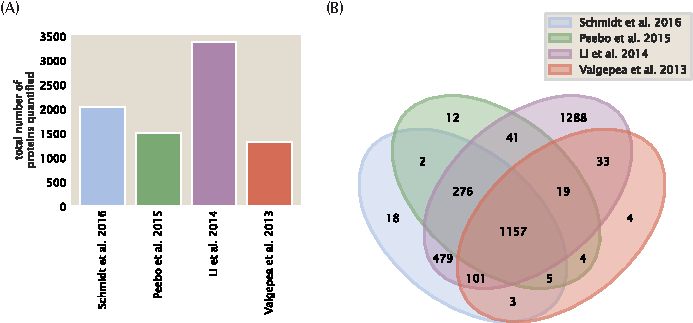
\includegraphics{SI_figs/intersections_venn.pdf}
        \caption{\textbf{Comparison of proteomic coverage across different data sets.}
        (A) Total number of unique proteins quantified in the data sets of
        \cite{valgepea2013, li2014, schmidt2016, peebo2015}. (2) Venn diagram
        showing the number of unique proteins and their intersections across each
        of the four data sets in (A). The intersection of all four data
        sets identifies 1157 proteins with measured protein copy number values.
        } \label{fig:venn}
    }
\end{figure*}

\section{Estimation of Cell Size and Surface Area}
\label{sec:protein_size_SV}
Since most of the proteomic data sets lack cell size (i.e. volume) measurements, we chose
instead to use a common estimate of size for any analysis requiring cell
size or surface area.  Since each of the data sets used either K-12 MG1655 or
its derivative, BW25113 (from the lab of Barry L. Wanner; the parent strain of
the Keio collection \citep{datsenko2000, baba2006}), we fit the MG1655 cell size
data from the supplemental material of \cite{si2017, si2019} using the optimize.curve\_fit function
from the Scipy python package \citep{2020scipynmeth}.

The average size measurements from each of their experiments are shown in Figure
\FIG{final_size_data_Si}, with  cell length and width shown in (A) and (B),
respectively. The length data was well described by the exponential function 0.5
$e^{1.09 \cdot \lambda}$ + 1.76 \textmu m, while the width data was well
described by 0.64 $e^{0.24 \cdot \lambda}$ \textmu m. In order to estimate cell
size we take the cell as a cylinders with two hemispherical ends \citep{si2017,
basan2015}. Specifically,  cell size  is estimated from,

\begin{equation}
V = \pi \cdot r^2 \cdot (l - 2r/3),
\label{eq:cell_size}
\end{equation}
where $r$ is half the cell width. A best fit to the data is described by 0.533
$e^{1.037 \cdot \lambda}$ \textmu m$^3$. Calculation of the cell surface area is
given by,

\begin{equation}
 S = \eta \cdot \pi (\frac{\eta \cdot \pi}{4} - \frac{\pi}{12})^{-2/3} V^{2/3},
 \label{eq:surface_area}
\end{equation}
where $\eta$ is the aspect ratio ($\eta$ = $l/w$) \citep{ojkic2019}.

\begin{figure}
		\centering
    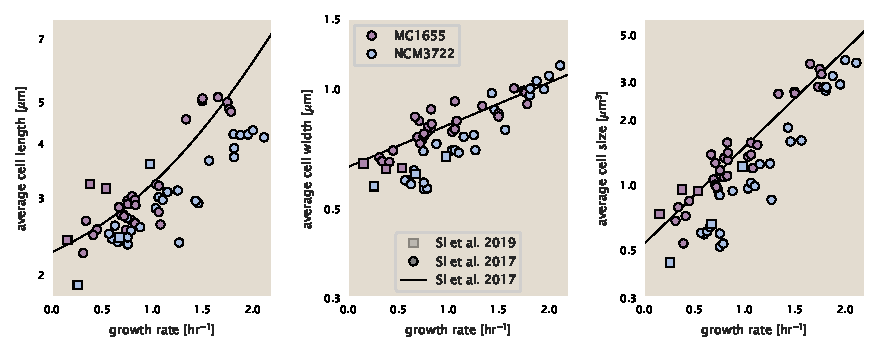
\includegraphics[width=1.0\textwidth]{SI_figs/Si_size_data_fit.pdf}
    \caption{\textbf{Summary of size measurements from Si \textit{et al.} 2017,
    2019.} Cell lengths and widths were measured from cell contours obtained from
    phase contrast images, and refer to the long and short axis respectively. (A)
    Cell lengths and (B) cell widths show the mean measurements reported (they
    report 140-300 images and 5,000-30,000 for each set of samples; which likely
    means about 1,000-5,000 measurements per mean value reported here since they
    considered about 6 conditions at a time). Fits were made to the  MG1655 strain
    data; length: 0.5 $e^{1.09 \cdot \lambda}$ + 1.76 \textmu m, width:  0.64
    $e^{0.24 \cdot \lambda}$ \textmu m. (C) Cell size, $V$, was calculated as
    cylinders with two hemispherical ends (Equation \ref{eq:cell_size}). The
    MG1655 strain data gave a best fit of 0.533 $e^{1.037 \cdot \lambda}$ \textmu m$^3$.}
  \label{fig:final_size_data_Si}
\end{figure}


\section{Estimation of Total Protein Content per Cell}
\label{sec:estimate_protein_per_cell}
In order to estimate total protein per cell for a particular growth rate, we
begin by estimating the cell size from the fit shown in Figure
\FIG{final_size_data_Si}(C) (0.533 $e^{1.037 \cdot \lambda}$ \textmu m$^3$). We
then estimate the total protein content from the total dry mass of the cell.
Here we begin by noting that  for almost the entire range of growth rates
considered here, protein, DNA, and RNA were reported to account for at least 90
\% of the dry mass (\cite{basan2015}). The authors also found that the total dry
mass concentration was roughly constant across growth conditions. Under such a
scenario, we can calculate the total dry mass concentration for protein, DNA,
and RNA, which is given by 1.1 g/ml x 30 \% x 90 \% or about $[M_P]$ = 300 fg
per fl. Multiplying this by our prediction of cell size gives the total dry mass
per cell.

However, even if dry mass concentration is relatively constant across growth
conditions, it is not obvious how protein concentration might vary due to
the substantial increase in rRNA at faster
growth rates (\cite{dai2016}). This is a well-documented result that arises from
an increase in ribosomal abundance at faster growth rates
(\cite{scott2010}). To proceed therefore rely on experimental
measurements of total DNA content per cell that also come from Basan \textit{et
al.}, and RNA to protein ratios that were measured in Dai \textit{et al.} (and
cover the entire range of growth conditions considered here). These are
reproduced in Figure \FIG{schmidt_adjustment_varying_conc}(A) and (B),
respectively.

Assuming that the protein, DNA, and RNA account for 90 \% of the total dry mass,
the protein mass can then determined by first subtracting the experimentally
measured DNA mass,  and then using the experimental estimate of the RNA to
protein ratio. The total protein per cell is will be related to the summed RNA
and protein mass by,

\begin{equation}
	M_{P} = \frac{[M_P + M_{RNA}]}{1 + (RP_{ratio})}.
\end{equation}
$(RP_{ratio}$ refers to the RNA to protein ratio as measured by Dai \textit{et
al.}. In Figure \FIG{schmidt_adjustment_varying_conc}(C) we plot the estimated
cellular concentrations for protein, DNA, and RNA from these calculations, and
in Figure \FIG{schmidt_adjustment_varying_conc}(D) we plot their total expected
mass per cell. This later quantity is the growth rate-dependent total protein
mass that was used to extimate total protein abundance across all data sets (and
summaried in \FIG{total_protein_final}(B)).


\begin{figure}
		\centering
    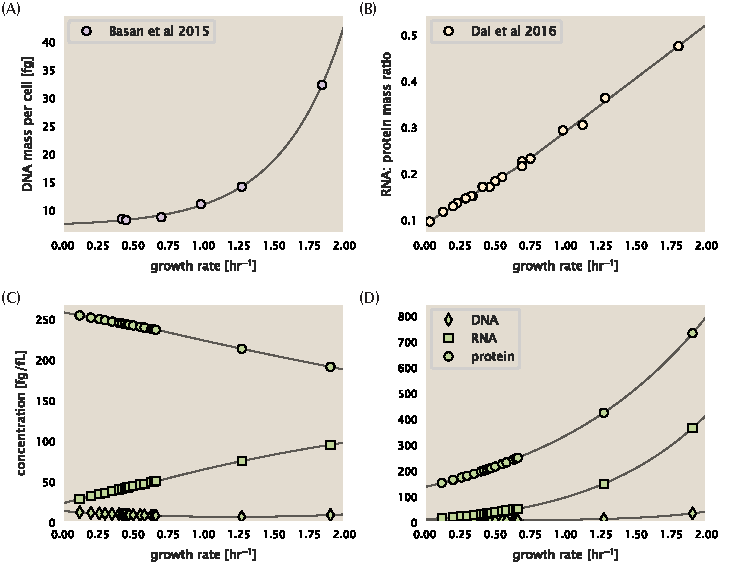
\includegraphics[width=1\textwidth]{SI_figs/schmidt_estimate_protein_RNA_DNA_corrections.pdf}
  \caption{{\bf Empirical estimate of cellular protein, DNA, and RNA as a
  function of growth rate.} (A) Measured DNA mass per cell as a function of
  growth rate, reproduced from Basan \textit{et al.} 2015. The data was fit to
  an exponential curve (DNA mass in fg per cell is given by 0.42 $e^{2.23 \cdot
  \lambda}$ + 7.2 fg per cell, where $\lambda$ is the growth rate in hr$^{-1}$).
  (B) RNA to protein measurements as a function fo growth rate. The data was for
  to two lines: for growth rates below 0.7 hr$^{-1}$, the RNA/protein ratio is
  0.18$\cdot \lambda$ + 0.093, while for growth rates faster than 0.7 hr$^{-1}$
  the RNA/protein ratio is given by 0.25$\cdot \lambda$ + 0.035. For (A) and (B)
  cells are grown under varying levels of nutrient limitation, with cells grown
  in minimal media with different carbon sources for the slowest growth
  conditions, and rich-defined media for fast growth rates. (C) Predictions of
  cellular protein, DNA, and RNA concentration.  (D) Total cellular mass
  predicted for protein, DNA, and RNA using the cell size predictions from Si
  \textit{et al.}. Symbols (diamond: DNA, square: RNA, circle: protein)
	show estimated values of mass concentration and mass per cell for the specific
	growth rates in \cite{schmidt2016}.
	 	}
  \label{fig:schmidt_adjustment_varying_conc}
\end{figure}

\section{Additional Considerations of Schmidt \textit{et al.} Data Set}
\label{sec:SI_schmidt}

While the data set from \cite{schmidt2016} remains a heroic effort that our
lab continues to return to as a resource, there were steps taken in their
calculation of protein copy number that we felt needed further
consideration. In particular, the authors made an assumption of constant
cellular protein concentration across all growth conditions and used
measurements of cell volume that appear inconsistent with an expected
exponential scaling of cell size with growth rate that is well-documented in
\textit{E. coli} (\cite{schaechter1958, taheriaraghi2015, si2017}).

We begin by looking at their cell volume measurements, which are shown in blue
in Figure \FIG{cell_size_literature}. As a comparison, we also plot cell sizes
reported in three other recent papers: measurements from Taheri-Araghi
\textit{et al.} and Si \textit{et al.} come from the lab of Suckjoon Jun, while
those from Basan \textit{et al.} come  from the lab of Terence Hwa.  Each set of
measurements used microscopy and cell segmentation to determine the length and
width, and then calculated cell size by treating the cell is a cylinder with two
hemispherical ends, as we considered in the previous section. While there is
notable discrepancy between the two research groups, which are both using strain
NCM3722, Basan \textit{et al.} found that this came specifically from
uncertainty in determining the cell width. This is prone to inaccuracy given the
small cell size and optical resolution limits (further described in their
supplemental text). Perhaps the more concerning point is that while each of
these alternative measurements show an exponential increase in  cell size at
faster growth rates, the measurements used by Schmidt \textit{et al.} appear to
plateau. This resulted in an analogous trend in their final reported total
cellular protein per cell as shown in Figure \FIG{schmidt_adjustment_summary}
(purple data points), and is in disagreement with other measurements of total
protein at these growth rates \citep{basan2015}.

\begin{figure}
		\centering{
    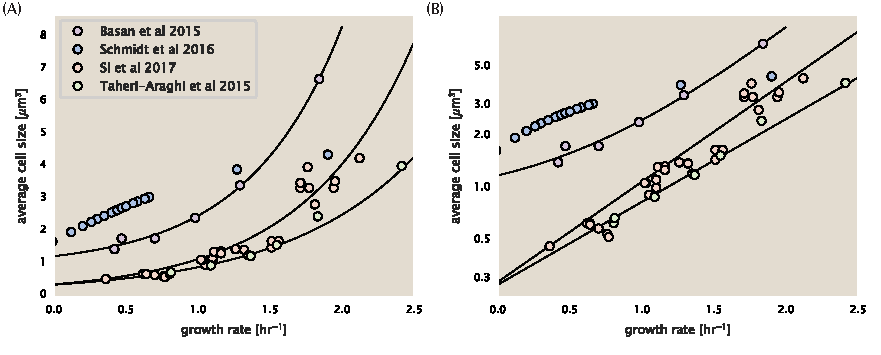
\includegraphics[width=1\textwidth]{SI_figs/size_data_lit.pdf}
  \caption{\textbf{Measurements of cell size as a function of growth rate.}
	 	(A) Plot of the reported cell sizes from several recent papers.  The data
	 	in blue come from Volkmer and Heinemann, 2011 (\cite{volkmer2011}) and were
	 	used in the work of Schmidt \textit{et al.}. Data from the lab of Terence Hwa
	 	are shown in purple (\cite{basan2015}), while the two data sets shown in green
	 	and red come from the lab of Suckjoon Jun (\cite{taheriaraghi2015,
	 	si2017}). (B) Same as in (A) but with the data plotted on a logarithmic
	 	y-axis to highlight the exponential scaling that is expected for \textit{E.
	 	coli}.}
  \label{fig:cell_size_literature}
  }
\end{figure}

Since it is not obvious how measurements of cell size influenced their reported
protein abundances, in the following subsections we begin by considering this
calculation. We then consider three different approaches to estimate the
growth-rate dependent total protein mass to compare with those values reported
from \cite{schmidt2016}. The results of this are summarized in
\FIG{cell_size_literature}(B), with the original values from both
\cite{schmidt2016} and \cite{li2014} shown in \FIG{cell_size_literature}(A) for
reference. For most growth conditions, we find that total protein per cell is
still in reasonable agreement. However, for the fastest growth conditions, with
glycerol + supplemented amino acids, and LB media, all estimates are
substantially higher than those originally reported. This is the main reason why
we chose to readjusted protein abundance as shown in
\FIG{total_protein_final}(B) (with the calculation described in section
\nameref{sec:estimate_protein_per_cell}).


\begin{figure}
		\centering
    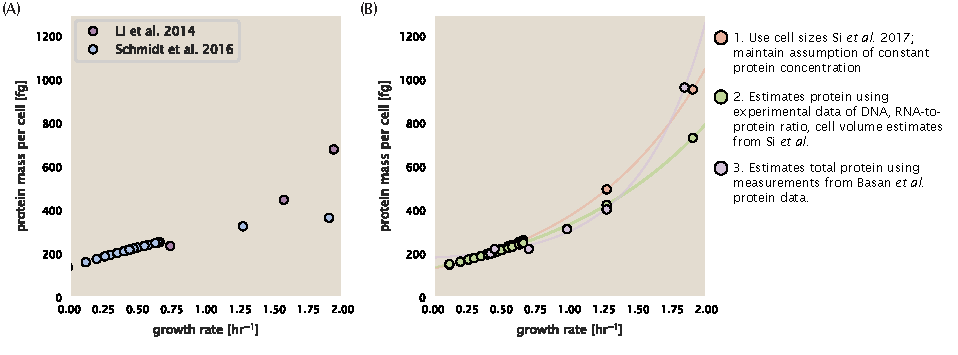
\includegraphics[width=1\textwidth]{SI_figs/schmidt_protein_corrections.pdf}
  \caption{{\bf Alternative estimates of total cellular protein for the growth conditions
    considered in Schmidt \textit{et al.}} (A) The original protein mass from
    Schmidt \textit{et al.} and Li \textit{et al.} are shown in purple and blue,
    respectively. (B) Three alternative estimates of total protein per cell.
		1.  \textit{light red}: Rescaling of total protein mass assuming a
    growth rate independent protein concentration and cell volumes estimated
    from Si \textit{et al.} 2017. 2. \textit{light green}:  Rescaling of total protein
    mass using estimates of growth rate-dependent protein concentrations and
    cell volumes estimated from Si \textit{et al.} 2017. Total protein per cell
		is calculated by assuming a 1.1 g/ml cellular mass density, 30\% dry mass, with
		90\% of the dry mass corresponding to DNA, RNA, and protein \citep{basan2015}. See
		\nameref{sec:estimate_protein_per_cell} for details on calculation. 3.\textit{light purple}: Rescaling
    of total protein mass using the experimental measurements from Basan
    \textit{et al.} 2015.
	 	}
  \label{fig:schmidt_adjustment_summary}
\end{figure}

\subsection{Effect of cell volume on reported absolute protein abundances}

As noted in section \nameref{sec:SI_exp_summary},
the authors calculated proteome-wide protein abundances by first determining
absolute abundances of 41 pre-selected proteins, which relied on adding
synthetic heavy reference peptides into their protein samples at known abundance.  This
absolute quantitation was performed in replicate for each growth condition.
Separately, the authors also performed a more conventional mass spectrometry
measurement for samples from each growth condition, which attempted to maximize
the number of quantified proteins but only provided relative abundances based on
peptide intensities. Finally, using their 41 proteins with absolute abundances
already determined, they then created calibration curves with which to relate
their relative intensity to absolute protein abundance for each growth
condition.  This allowed them to estimate absolute protein abundance for all
proteins detected in their proteome-wide data set. Combined with their flow
cytometry cell counts, they were then able to determine absolute abundance of
each protein detected on a per cell basis.

While this approach provided absolute abundances, another necessary step
to arrive at total cellular protein was to account for any protein loss during
their various protein extraction steps. Here the authors attempted to determine
total protein separately using a BCA protein assay.  In personal communications,
it was noted that determining reasonable total protein abundances by BCA across
their array of growth conditions  was particularly troublesome. Instead, they
noted confidence in their total protein measurements for cells grown in M9
minimal media + glucose and  used this as a reference point with which to
estimate the total protein for all other growth conditions.

For cells grown in M9 minimal media + glucose an average total mass of $M_P$ =
240 fg per cell was measured. Using their reported cell volume, reported as
$V_{orig}$ = 2.84 fl, a cellular protein concentration of $[M_P]_{orig}$ =
$M_P/V_{orig}$ = 85 fg/fl. Now, taking the assumption that cellular protein
concentration is relatively independent of growth rate, they could then estimate
the total protein mass for all other growth conditions from,

\begin{equation}
	M_{P\_i} = [M_P]_{orig} \cdot V_{i}
\end{equation}
where $M_{P_i}$ represents the total protein mass per cell and $V_{i}$ is the
cell volume for each growth condition $i$ as measured in Volkmer and Heinemann,
2011. Here the thinking is that the values of $M_{P_i}$ reflects the total
cellular protein for growth condition $i$, where any discrepancy from their
absolute protein abundance is assumed to be due to protein loss during sample
preparation. The protein abundances from their absolute abundance measurements
noted above were therefore scaled to their estimates and are  shown in Figure
\FIG{schmidt_adjustment_summary} (purple data points).

If we instead consider the cell volumes predicted in the work of Si \textit{et
al.}, we again need to take growth in M9 minimal media + glucose as a reference
with known total mass, but we can follow a similar approach to estimate total
protein mass for all other growth conditions. Letting  $V_{Si\_glu}$ = 0.6 fl be
the predicted cell volume, the cellular protein concentration becomes
$[M_P]_{Si}$ = $M_P/V_{Si\_glu}$ = 400 fg/fl. The new total protein mass per
cell can then be calculated from,

\begin{equation}
	M_{P\_i}' = [M_P]_{Si} \cdot V_{Si\_i}
\end{equation}
where $M_{P_i}'$ is the new protein mass prediction, and $V_{Si_i}$ refers to
the new volume prediction for each condition $i$, These are shown as red data points in
Figure \FIG{schmidt_adjustment_summary}(B).


\subsection{Relaxing assumption of constant protein concentration across growth conditions}
We next relax the assumption that cellular protein concentration is constant and
instead, attempt to  estimate it using experimental data. Here we use the
estimation of total protein mass per cell detailed in section
\nameref{sec:estimate_protein_per_cell} for all data points in the
\cite{schmidt2016} data set. The green data points in
\FIG{schmidt_adjustment_summary}(B) show this prediction, and this represents
the approach used to estimate total protein per cell for all data sets.


\subsection{Experimental measurements of total protein from Basan \textit{et al.} 2015.}

One of the challenges in our estimates in the preceding  sections is the need to
estimate protein concentration and cell volumes. These are inherently difficult
to to accurately due to the small size of \textit{E. coli}. Indeed, for all the
additional measurements of cell volume included in Figure
\FIG{cell_size_literature}, no measurements were performed for cells growing
at rates below 0.5 $hr^{-1}$. It therefore remains to be determined whether our
extrapolated cell volume estimates are appropriate, with the possibility that
the logarithmic scaling of cell size might break down for slower growth.

In our last approach we therefore attempt to estimate total protein using
experimental data that required  no estimates of concentration or cell volume.
Specifically, in the work of  Basan \textit{et al}, the authors measured total
protein per cell for a broad range of growth rates (reproduced in Figure
\FIG{schmidt_adjustment_basan}). These were determined by first measuring
bulk protein from cell lysate, measured by the colorimetric Biuret method
(\cite{You2013}), and then abundance per cell was calculated from cell counts
from either plating cells or a Coulter counter. While it is unclear why Schmidt
\textit{et al.} was unable to take a similar approach, the results from Basan
\textit{et al} appear more consistent with our expectation that cell mass will
increase exponentially with faster growth rates. In addition, although they do
not consider growth rates below about 0.5 $hr^{-1}$, it is interesting to note
that the protein mass per cell appears to plateau to a minimum value at slow
growth. In contrast, our estimates using cell volume so far have predicted that
total protein mass should continue to decrease slightly for slower growing
cells. By fitting this data to an exponential function dependent on growth rate,
we could then estimate the total protein per cell for each growth condition
considered by \cite{schmidt2016}. These are plotted as red data points in
\FIG{schmidt_adjustment_summary}(B).


\begin{figure}
		\centering
    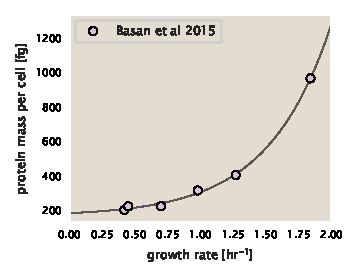
\includegraphics[width=0.5\textwidth]{SI_figs/schmidt_protein_estimate_basan.pdf}
  \caption{{\bf Total cellular protein reported in Basan \textit{et al.} 2015.}
  Measured protein mass as a function of growth rate as reproduced from Basan
  \textit{et al.} 2015, with cells grown under different levels of nutrient
  limitation. The data was fit to an exponential curve  where protein mass in fg
  per cell is given by 14.65 $e^{2,180 \cdot \lambda}$ + 172 fg per cell, where
  $\lambda$ is the growth rate in hr$^{-1}$).}
  \label{fig:schmidt_adjustment_basan}
\end{figure}

\section{Calculation of Complex Abundance}

All protein data quantified the abundance of individual proteins per cell.
However, this work requires estimates on the abundance of individual protein
\textit{complexes}, rather than the copy number of individual proteins. In our
analysis of the protein copy number data, it became clear that the reported copy
numbers do not always align with those based on reported stiochometry. As one
example of this, the F-O subunit of ATP synthase consists of three protein
subunits with a stiochometry of [AtpB][AtpF]$_2$[AtpE]$_{10}$ (also referred to
as subunits a, b, and c, respectively). In the experimental data of
\cite{schmidt2016}, the values deviate from this quite substantially, with
approximately 1000 AtpB, 9000 AtpF, and 300 AtpE reported per cell (minimal
media + glucose growth condition).  This highlights the technical challenges
that still remain in our ability to quantify cellular composition, particularly
for membrane-bound proteins like the ATP synthase complex considered here.  In
this section, we outline the approach we used to annotate proteins as part of
each macromolecular complex and how we used averaging across the individual
protein measurements to estimate an absolute complex abundances per cell.

Protein complexes, and proteins individually, often have a variety of names,
both longform and shorthand. As individual proteins can have a variety of
different synonyms, we sought to ensure that each protein annotated in the
data sets used the same synonym. To do use, we relied heavily on the EcoCyc
Genomic Database \citep{keseler2017}.  Each protein in available data sets
included an annotation of one of the gene name synonyms as well as an
accession ID -- either a UniProt or Blattner "b-number". We programmatically
matched up individual accession IDs between the proteins in different data sets.
In cases where accession IDs matched but the gene names were different, we
manually verified that the gene product was the same between the datasets and
chose a single synonym.  All code used  in the data cleaning and unification
procedures can be found on the associated
\href{https://github.com/rpgroup-pboc/growth_limits}[GitHub repository]
(DOI:XXX) associated with this paper as well as on the associated
\href{https://rpgroup.caltech.edu/growth_limits}{paper website}.

With each protein conforming to a single identification
scheme, we then needed to identify the molecular complexes each protein was a
member of. Additionally, we needed to identify how many copies of each protein
were present in each complex (i.e. the subunit copy number) and compute the
estimated abundance complex that accounted for fluctuations in subunit
stoichiometry. To map proteins to complexes, we accessed the
EcoCyc \textit{E. coli} database \cite{keseler2017} using PathwayTools version
23.0 \cite{karp2019}. With a license for PathWay Tools, we
mapped each unique protein to its annotated complexes via the
BioCyc Python package. As we mapped each protein with \textit{all} of its
complex annotations, there was redundancy in the dataset. For example, ribosomal
protein L20 (RplT) is annotated to be a component of the 50S ribosome (EcoCyc
complex \texttt{CPLX-03962}) as well as a component of the mature 70S ribosome
(EcoCyc complex \texttt{CPLX-03964}).

In addition to the annotated complex, we collected information on the
stoichiometry of each macromolecular complex. For a complex with $N_\text{subunits}$ protein species,
for each protein subunit $i$ we first calculate the number of complexes that
\textit{could} be formed given the measured protein copy numbers per cell,
\begin{equation}
    N_\text{complex}(\text{subunit i}) = \frac{P_\text{subunit i}^\text{(measured)}}{m_\text{subunit i}}.
    \label{eq:subunit_max}
\end{equation}
Here, $P_\text{subunit i}^\text{(measured)}$ refers to the measured protein copy number of species $i$,
and $m$ refers to the number of monomers present for that protein in the complex. For example, the 70S mature ribosome complex has 55 protein components, all of
which are present in a single copy except L4 (RplL), which is present in 4
copies ($m$ = 4). For each ribosomal protein, we then calculate the  maximum number of
complexes that could be formed using \EQ{subunit_max}. This example, along with
example from 5 other macromolecular complexes, can be seen in
\FIG{complex_counting}.

It is important to note that measurement noise, efficiency of protein
extraction, and differences in protein stability will mean that the precise value of each
calculation will be different for each component of a given complex. Thus, to
report the total complex abundance, we use the arithmetic mean of
across all subunits in the complex,
\begin{equation}
   \langle N_\text{complex} \rangle = \frac{1}{N_\text{subunits}}\sum\limits_i^{N_\text{subunits}} \frac{P_{i}^\text{(measured)}}{m_\text{subunit i}}.
   \label{eq:complex_count}
\end{equation}
in \FIG{complex_counting}, we show this mean value as a grey line for a variety
of different complexes. Additionally, we have built an interactive figure
accessible on the \href{https://www.rpgroup.caltech.edu/growth_limits}{paper
website} where the validity of this approach can be examined for any complex
with more than two subunits (thus, excluding monomers and dimers).

\begin{figure}
    \begin{fullwidth}
        \centering{
            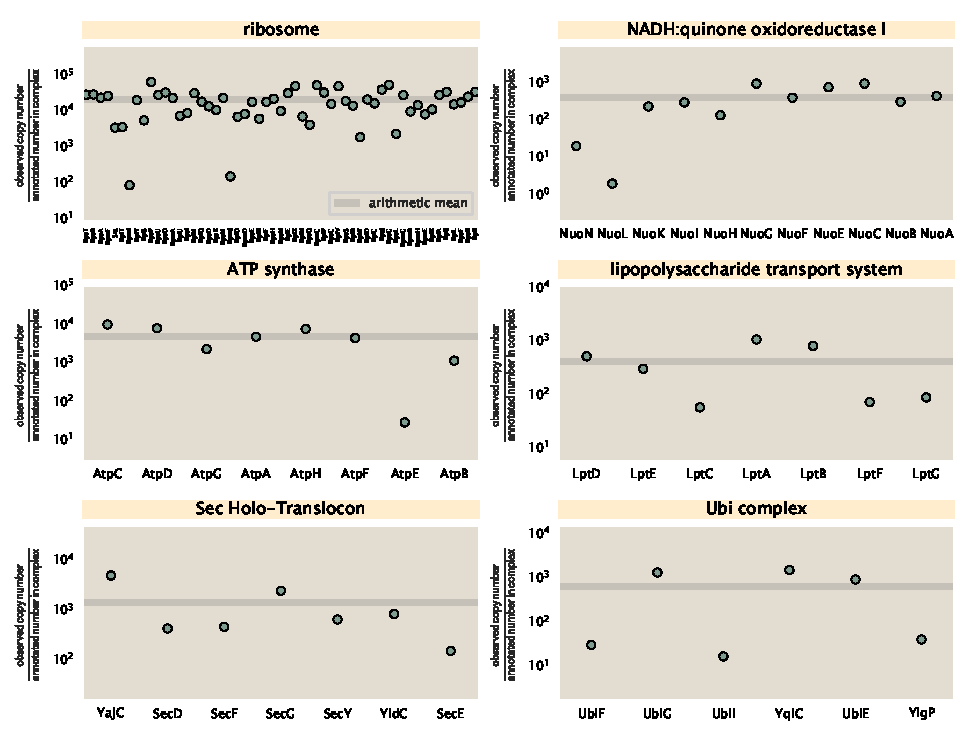
\includegraphics{SI_figs/figSX_subunit_counting.pdf}
            \caption{\textbf{Calculation of the mean complex abundance from
            measurements of single subunits.} Six of the largest complexes (by
            number of subunits) in \textit{E. coli}. Points correspond to the
            maximum number of complexes that can be formed given measurement of
            that individual protein. Solid grey line corresponds to the
            arithmetic mean across all subunits. These data correspond to
            measurements from \cite{schmidt2016} in a glucose-supplemented
            minimal growth medium.}
            \label{fig:complex_counting}
        }
    \end{fullwidth}
\end{figure}

\section{Extending Estimates to a Continuum of Growth Rates}
\label{sec:SI_continuum_est}
In the main text, we considered a standard stopwatch of 5000 s to estimate the
abundance of the various protein complexes considered. In addition to point
estimates, we also showed the estimate as a function of growth rate as
transparent grey curves. In this section, we elaborate on this continuum
estimate, giving examples of estimates that scale with either cell volume, cell
surface area, or number of origins of replication.

\subsection{Estimation of the total cell mass}
For many of the processes estimated in the main text we relied on a cellular dry
mass of $\approx 300$ fg from which we computed elemental and protein fractions
using knowledge of fractional composition of the dry mass. At modest growth
rates, such as the 5000 s doubling time used in the main text, this is a
reasonable number to use as the typical cell mass is $\approx$ 1 pg and
\textit{E. coli} cells can approximated as 70\% water by volume. However, as we
have shown in the preceding sections, the cell size is highly dependent on the growth rate. This means that a dry mass of 300
fg cannot be used reliably across all growth rates.

Rather, using the phenomenological  description of cell volume scaling
exponentially with growth rate, and using a rule-of-thumb of a cell buoyant
density of $\approx 1.1$ pg / fL (BNID: 103875), we can calculate the cell dry mass across a
range of physiological growth rates as
\begin{equation}
    m_\text{cell} \approx \rho V(\lambda) \approx \rho ae^{\lambda * b}
    \label{eq:def_mcell}
\end{equation}
where $a$ and $b$ are constants with units of \textmu m$^3$  and hr,
respectively. The value of these constants can be estimated from the careful
volume measurements performed by \cite{si2017}, as considered in Appendix \nameref{sec:protein_size_SV} earlier.

\subsection{Complex Abundance Scaling With Cell Volume}
Several of the estimates performed in the main text are implicitly dependent
on the cell volume. This includes processes such as ATP utilization and, most
prominently, the transport of nutrients, whose demand will be proportional to the volume
of the cell. Of the latter, we estimated the
number of transporters that would be needed to shuttle enough carbon,
phosphorus, and sulfur across the membrane to build new cell mass. To do so,
we used elemental composition measurements combined with a 300 fg cell dry
mass to make the point estimate. As we now have a means to estimate the total
cell mass as a function of volume, we can generalize these estimates across
growth rates.

Rather than discussing the particular details of each transport system, we will
derive this scaling expression in very general terms. Consider that we wish to
estimate the number of transporters for some substance $X$, which has been
measured to be made up some fraction of the dry mass, $\theta_X$. If we assume
that, irrespective of growth rate, the cell dry mass is relatively constant
\citep{basan2015} and $\approx$ 30\% of the total cell mass, we can state that
the total mass of substance $X$ as a function of growth rate is
\begin{equation}
m_X \approx 0.3 \times \rho V(\lambda) \theta_X,
\label{eq:m_x}
\end{equation}
where we have used $\rho V(\lambda)$ as an estimate of the total cell mass,
defined in Equation \ref{eq:def_mcell}. To convert this to the number of units $N_X$ of substance
$X$ in the cell, we can use the formula weight $w_X$ of a single unit of $X$ in
conjunction with Equation \ref{eq:m_x},
\begin{equation}
    N_X \approx \frac{m_X}{w_X}.
    \label{eq:n_x}
\end{equation}

To estimate the number of transporters needed, we make the approximation that
loss of units of $X$ via diffusion through porins or due to the permeability of
the membrane is negligible  and that a single transporter complex can transport
substance $X$ at a rate $r_X$. As this rate $r_X$  is in units of $X$ per time
per transporter, we must provide a time window over which the transport process
can occur. This is related to the cell doubling time $\tau$, which can be
calculated from the the growth rate $\lambda$ as $\tau = \log(2) / \lambda$.
Putting everything together, we arrive at a generalized transport scaling
relation of
\begin{equation}
N_\text{transporters}(\lambda) = \frac{0.3 \times \rho V(\lambda)\theta_X}{w_X r_X \tau}.
\label{eq:transporter_continuum}
\end{equation}

This function is used to draw the continuum estimates for the number of
transporters seen in Figures 2 and 3 as transparent grey curves. Occasionally,
this continuum scaling relationship will not precisely agree with the point
estimate outlined in the main text. This is due to the choice of $\approx$ 300 fg
total dry mass per cell for the point
estimate, whereas we considered more precise values of cell mass in the continuum estimate. We
note, however, that both this scaling relation and the point estimates are meant
to describe the order-of-magnitude observed, and not the predict the exact
values of the abundances.

Equation \ref{eq:transporter_continuum} is a very general relation for processes where the
cell volume is the "natural variable" of the problem. This means that, as the
cell increases in volume, the requirements for substance $X$ also scale with
volume rather than scaling with surface area, for example. So long as the rate
of the process, the fraction of the dry mass attributable to the substance, and
the formula mass of the substance is known, Equation \ref{eq:transporter_continuum} can be
used to compute the number of complexes needed. For example, to compute the
number of ATP synthases per cell, Equation \ref{eq:transporter_continuum} can be slightly
modified to the form
\begin{equation}
    N_\text{ATP synthases}(\lambda) = \frac{0.3 \times \rho V(\lambda)\theta_{protein}N_\text{ATP}}{w_{AA} r_\text{ATP} \tau},
\end{equation}
where we have included the term $N_\text{ATP}$ to account for the number of ATP
equivalents needed per amino acid for translation ($\approx$ 4, BNID: 114971),
and $w_{AA}$ is the average mass of an amino acid. The grey curves in Figure 4
of the main text were made using this type of expression.

\subsection{A Relation for Complex Abundance Scaling With Surface Area}
In our estimation for the number of complexes needed for lipid synthesis and
peptidoglycan maturation, we used a particular estimate for the cell surface
area ($\approx$ 5 \textmu$m$, BNID: 101792) and the fraction of dry mass
attributable to peptidoglycan ($\approx$ 3\%, BNID: 101936). Both of these
values come from glucose-fed \textit{E. coli} in balanced growth. As we are
interested in describing the scaling as a function of the growth rate, we must
also consider how these values scale with cell surface area, which is the natural
variable for these types of processes. In the coming paragraphs, we highlight
how we incorporate a condition-dependent surface area into our calculation of
the number of lipids and murein monomers that need to be synthesized and
crosslinked, respectively.

\subsubsection{Number of Lipids}
To compute the number of lipids as a function of growth rate, we make the
assumption that some features, such as the surface area of a single lipid
($A_\text{lipid} \approx$ 0.5 nm$^2$, BNID: 106993) and the total fraction of the membrane
composed of lipids ($\approx$ 40\%, BNID: 100078) are independent of the growth
rate. Using these approximations combined with Equation \ref{eq:surface_area}, and
recognizing that each membrane is composed of two leaflets, we can
compute the number of lipids as a function of growth rate as

\begin{equation}
    N_\text{lipids}(\lambda) \approx \frac{4\,\text{leaflets} \times 0.4 \times
    \eta\pi\left(\frac{\eta\pi}{4} -
    \frac{\pi}{12}\right)^{-2/3}V(\lambda)^{2/3}}{A_\text{lipid}}
\end{equation}
where $\eta$ is the length-to-width aspect ratio and $V$ is the cell volume.

\subsubsection{Number of Murein Monomers}
In calculation of the number of transpeptidases needed for maturation of the
peptidoglycan, we used an empirical measurement that $\approx$ 3\% of the dry
mass is attributable to peptidoglycan and that a single murien monomer is
$m_\text{murein} \approx$ 1000 Da. While the latter is independent of growth rate, the former is
not. As the peptidoglycan exists as a thin shell with a width of $w \approx 10$
nm encapsulating the cell, one would expect the number of murein monomers scales
with the surface area of this shell. In a similar spirit to our calculation of
the number of lipids, the total number of murein monomers as a function of
growth rate can be calculated as
\begin{equation}
N_\text{murein monomers}(\lambda) \approx \frac{\rho_\text{pg} w \eta\pi\left(\frac{\eta\pi}{4} -
    \frac{\pi}{12}\right)^{-2/3}V(\lambda)^{2/3}}{m_\text{murein}},
\end{equation}
where $\rho_\text{pg}$ is the density of peptidoglycan.


\subsection{Complex Abundance Scaling With Number of Origins, and rRNA Synthesis}
While the majority of our estimates hinge on the total cell volume or surface
area, processes related to the central dogma, namely DNA replication and
synthesis of rRNA, depend on the number of chromosomes present in the cell. As
discussed in the main text, the ability of \textit{E. coli} to parallelize the
replication of its chromosome by having multiple active origins of replication
is critical to synthesize enough rRNA, especially at fast growth
rates. Derived in \cite{si2017} and reproduced in the main text and Appendix \nameref{sec:SI_ori} below, the average number of
origins of replication at a given growth rate can be calculated as
\begin{equation}
\langle\# \text{ori} \rangle \approx 2^{t_\text{cyc} \lambda / \ln 2}
\label{eq:nori}
\end{equation}
where $t_\text{cyc}$ is the total time of replication and division. We can make
the approximation that $t_\text{cyc} \approx$ 70 min, which is the  time from
the initiation of chromosomal replication until division. This time corresponds to
the sum of the so-called C and D periods of the cell cycle, which correspond to
the time it takes to replicate the entire chromosome (C period) and the time
from completion to eventual division (D period) \cite{helmstetter1968}.

In the case of rRNA synthesis, the majority of the rRNA operons are surrounding
the origin of replication. Thus, at a given growth rate $\lambda$, the average
dosage of rRNA operons per cell $D_\text{rRNA}$ is
\begin{equation}
D_\text{rRNA}(\lambda) \approx N_\text{rRNA operons} \times 2^{t_{cyc} \lambda / \ln 2}.
\label{eq:rRNA_dosage}
\end{equation}

This makes the approximation that \textit{all} rRNA operons are localized around
the origin. In reality, the operons are some distance away from the origin,
making Equation \ref{eq:rRNA_dosage} an approximation \citep{dennis2004}.

In the main text, we stated that at a growth rate of 0.5 hr$^{-1}$, there is
$\approx$ 1 chromosome per cell. While a fair approximation, Equation \ref{eq:nori}
illustrates that is not precisely true, even at slow growth rates. In estimating
the number of RNA polymerases as a function of growth rate, we consider that
regardless of the number of rRNA operons, they are all sufficiently loaded with
RNA polymerase such that each operon produces one rRNA per second. Thus, the
total number of RNA polymerase as a function of the growth rate can be
calculated as
\begin{equation}
    N_\text{RNA polymerase}(\lambda) \approx L_\text{operon}D_\text{rRNA}\rho_\text{RNA polymerase},
\end{equation}
where $L_\text{operon}$ is the total length of an rRNA operon ($\approx$ 4500
bp) and $\rho_\text{RNA polymerase}$ is packing density of RNA polymerase on a
given operon, taken to be 1 RNA polymerase per 80 nucleotides.

\section{Estimation of $\langle$\#ori$\rangle$ / $\langle$\#ter$\rangle$ and $\langle$\#ori$\rangle$.}

\textit{E. coli} shows robust scaling of cell size with the average the number
of origins $\langle$\#ori$\rangle$ per cell \citep{si2017}. Since protein makes
up a  majority of the cell's dry mass, the change is cell size is also a
reflection of the changes in proteomic composition and total abundance across
growth conditions. Given the potential constraints on rRNA synthesis and changes
in ribosomal copy number with $\langle$\#ori$\rangle$, it becomes important to
also consider how protein copy numbers vary with the state of chromosomal
replication. This is particularly true  when trying to make sense of the changes
in ribosomal fraction and growth-rate dependent changes in proteomic composition
at a  mechanistic level.  As considered in the main text, it is becoming
increasingly apparent that regulation through the secondary messengers (p)ppGpp
may act to limit DNA replication and also reduce ribosomal activity in poorer
nutrient conditions.  In this context, both $\langle$\#ori$\rangle$, as well as
the $\langle$\#ori$\rangle$ / $\langle$\#ter$\rangle$ ratio become important
parameters to consider and keep tract of. An increase in $\langle$\#ori$\rangle$
/ $\langle$\# ter$\rangle$ ratio  in particular, causes a relatively higher gene
dosage in rRNA and r-protein genes due to skew in genes near the origin, where
the majority of these are located

In the main text we estimated the change in $\langle$\#ori$\rangle$ with growth
rate using the nutrient-limited wild-type cell data from \cite{si2017}. We
consider their measurements of DNA replication time ($t_{C}$, 'C' period of
cell division), total cell cycle time ($t_{cyc}$, 'C' + 'D' period of cell
division), and doubling time $\tau$ from wild-type \textit{E. coli} growing
across a range of growth conditions. Here we show how we  esimate this
parameter, as well as the $\langle$\#ori$\rangle$ / $\langle$\# ter$\rangle$
ratio from their data.  We begin by considering $\langle$\#ori$\rangle$. If the
cell cycle time takes longer  than the time of cell division, the cell will need
to initiate DNA replication  more often than its rate of division, $2^{\lambda
t} = 2^{ln(2) \cdot t/ \tau}$ to maintain steady-state growth. Cells will need
to do this in proportion to the ratio $\lambda_{cyc} / \lambda =  t_{cyc}/\tau$,
and the number of origins per cell (on average) is then given by $2^{t_{cyc}/
\tau}$.   The average number of termini will in contrast depend on the lag time
between  DNA replication and cell division, $t_{D}$, with
$\langle$\#ori$\rangle$ / $\langle$\# ter$\rangle$ ratio = $2^{t_{cyc}/ \tau -
t_{D}/ \tau} =  2^{t_{C}/ \tau}$.

In Figure \ref{fig:Si_Cm}(A) and (B) we plot the measured $t_{C}$ and $t_{cyc}$
values versus the doubling time from \cite{si2017}. The authors estimated
$t_{C}$ by marker frequency analysis using qPCR, while  $t_{cyc} = t_{C} +
t_{D}$ were inferred from $t_{C}$ and $\tau$. In the plots we see that both
$t_{C}$ and $t_{cyc}$ reach a minimum  at around 40 and 75 minutes,
respectively. For a C period of 40 minutes, this would correspond to a maximum
rate of elongation of about 1,000 bp/sec. Since we lacked a specific model to
describe how each of these parameters vary with growth condition, we assumed
that they were linearly dependent on the doubling time. For each parameter,
$t_{C}$ and $t_{cyc}$, we split them up into two domains corresponding to poorer
nutrient conditions and rich nutrient conditions (cut off at $\tau \approx$ 40
minutes where chromosomal replication becomes nearly constant). The fit lines
are shown as solid black lines. In Figure \ref{fig:Si_Cm}(C) and (D) we also
show $t_{C}$ and $t_{cyc}$ as a function of growth rate $\lambda$ along with our
piecewise linear fits, which match the plots in the main text.


\begin{figure}
    \begin{fullwidth}
        \centering{
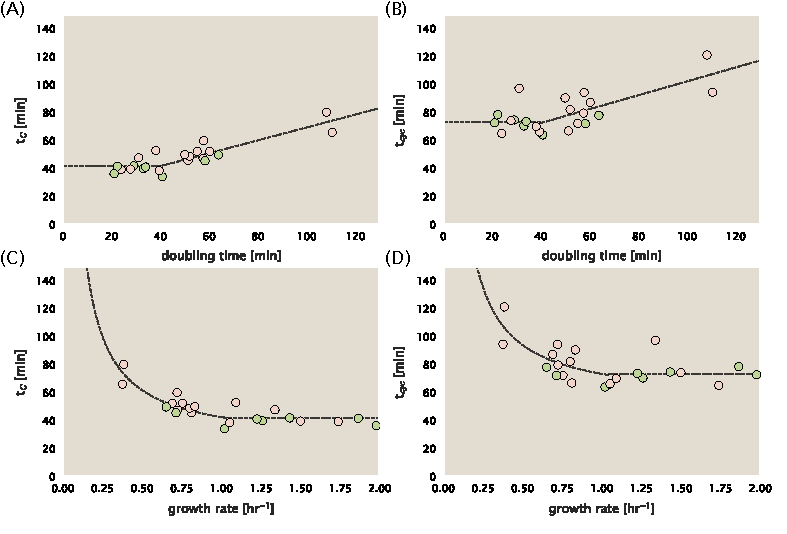
\includegraphics{SI_figs/supplemental_ori_ter.pdf} \caption{\textbf{Estimation of
    $\langle$\#ori$\rangle$ / $\langle$\# ter$\rangle$ and
    $\langle$\#ori$\rangle$ using data from Si \textit{et al.} (2017).} (A) and
    (B) plot the reported $t_{C}$ and $t_{cyc}$ as a function  of cell doubling
    time $\tau$, respectively. The dashed lines show a piecewise fit to  the
    data. For short doubling times (rich media), $t_{C}$ and $t_{cyc}$ are
    assumed  constant. At the transition, taken to occur at 40 minutes, the
    dashed line corresponds  to an assumed proportional increase in each
    parameter as a function of the doubling time. (C) and (D) plot the same data
    as in (A) and (B), but as a function of growth rate, given by $\lambda = ln(2)/\tau$.}
\label{fig:Si_tC_tcyc} }
\end{fullwidth}
\end{figure}

\section{Calculation of active ribosomal fraction.}

In the main text we used the active ribosomal fraction $f_a$ that was reported
in the work of \cite{dai2016} to estimate the active ribosomal mass fraction
$\Phi_R \times f_a$ across growth conditions. We lacked any specific model to
consider how  $f_a$ should vary with growth rate, and instead find that the data
is well-approximated by fitting to an exponential curve ($f_a$ = -0.889 $e^{4.6
\cdot \lambda}$ + 0.922; dashed line in inset of \FIG{ribosome_limit}(C)). We
use this function to estimate $f_a$ for each of the data points shown in
\FIG{ribosome_limit}(C).


% of actively translating ribosomes across
% the different datasets available based on the growth-rate dependent measurements from the work
% of \citep{dai2016}. Here we provide additional details on how $f_a$ was initially determined,
% and how we have used it to estimate the active ribosomal fraction for each data set.

% In the work of \citep{dai2016}, the authors independently measured the
% translation rate, ribosomal abundance (via the total RNA-to-protein ratio), and
% growth rate $\lambda$ across a vast range of growth conditions (growth rates spanning ~ 0
% - 2 h$^{-1}$). By requirements of mass balance, and an assumption that cells are doubling their
% proteome with each cell division under steady-state growth, we expect,
%
% \begin{equation}
%   r_t \cdot R  \lambda \cdot N_{aa}.
% \end{equation}
% $r_t$ is the translation elongation rate, $R$ is the number of ribosomes, and $N_{aa}$ is the number of peptide bonds that must be formed to double the cell's protein mass. An important observation from the work of \citep{dai2016} was that their measured translation rates and ribosomal abundance were incompatible with this expectation. This was particularly true at slow growth (below about 0.7 h$^{-1}$). The explanation arrived at by the authors is that cells are regulating the fraction of ribosomes that are translating. As further support for this idea, sublethal concentrations of chloramphenicol caused a further decrease in the apparent
% fraction of actively translating ribosomes.
%
% In Figure X we show the reported values of $f_a$ as a function of growth rate
%
% in order to maintain
%
%
%  \cdot R \cdot f_a$ $N_{aa}This corresponds to Equation 3 in the main text, where the
%
% estimate the fraction


% \section{Average protein expression across the chromosome.}
%
% In Figure 7(B) of the main text we plotted the average protein copy number along
% \textit{E. coli}'s chromosome using a boxcar averaging (i.e. running average)
% window of 0.5 Mb. This means that at each position on the chromosome, proteins
% with a transcription start site that were +/- 0.25 Mb from that position
% were  included in the calculated average. For \textit{E. coli},
% position 0 bp does not correspond the location of the origin and we  keep to
% this convention, using the reported positional information from EcoCyc. Since
% the chromosome is circular, when calculating the  average at positions  near the
% end positions (i.e. near either 0 bp or 4.6 Mb) we include the copy numbers
% on opposing ends.  For example, calculating the average for position 0 bp would
% include the range from 4.1 Mb to 0.25 Mb).  Here we provide some additional
% analysis to show how the absolute copy numbers compare across growth conditions,
% as well as the effect of the specific averaging window size.
%
% In the main text we centered each data set according to the mean average in order
% to  compare the relative changes in copy number along the length of the
% chromosome in each data set. In reality, there is also a correlation between the
% total genomic content and protein copy number, which increases at faster growth.
% This is shown in Figure \ref{fig:supplemental_boxcar_1}(A), where we plot the boxcar average from each
% growth condition without rescaling each about their mean values.
%
% \begin{figure}
%     \begin{fullwidth}
%         \centering{
% 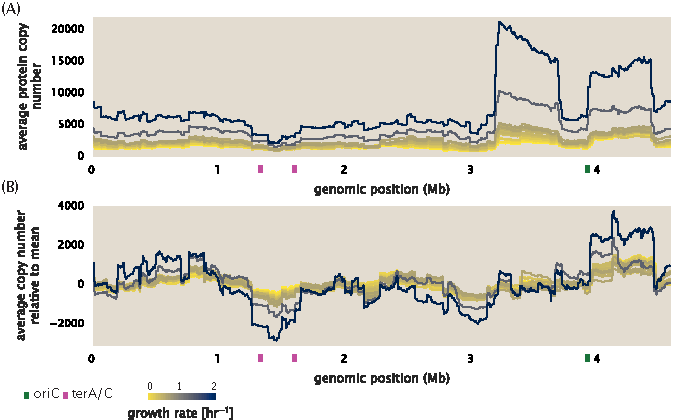
\includegraphics{SI_figs/supplemental_boxcar1.pdf} \caption{\textbf{Position-dependent protein expression at different growth rates.} (A) Protein copy number is reported along the length of the chromosome using a boxcar averaging, with window size of 0.5 Mb.
%   (B)The boxcar average protein copy number, shifted relative to the mean value for each
%   growth conditions, is show for a window size of 0.5 Mb. In this plot, all ribosomal
%   proteins and elongation factor EF-Tu were excluded in the analysis.}
% \label{fig:supplemental_boxcar_1} }
% \end{fullwidth}
% \end{figure}
%
% One of the challenges in interpreting this analysis is that the protein copy
% numbers for a small subset of proteins vary dramatically as a function of growth
% rate. This is particularly true for ribosomal proteins. In order to check
% whether the result is due simply due to the change in ribosomal copy number, we
% repeated the analysis with all ribosome proteins, and the translation elongation
% factor EF-Tu removed (Figure \ref{fig:supplemental_boxcar_1}(B)). Indeed we still
% see a skew in  protein abundance, with higher overall expression at the origin.
%
% The other important parameter in this analysis is the size of the averaging
% window, which we took at 0.5 Mb. In Figure \ref{fig:supplemental_boxcar_2} we show
% the  results when using averaging window sizes of 0.05 Mb, 0.25 Mb, 0.5 Mb, 1
% Mb, and 2 Mb. Aside from the smallest window size of 0.05 Mb, the analysis seems
% to show a similar result, with proteins near the origin showing highest
% expression. For the window size of  0.05 Mb, the copy numbers become much
% noisier due to the large differences in protein copy number  that are observed
% irrespective of the specific growth rate.
%
% \begin{figure}
%     \begin{fullwidth}
%         \centering{
% 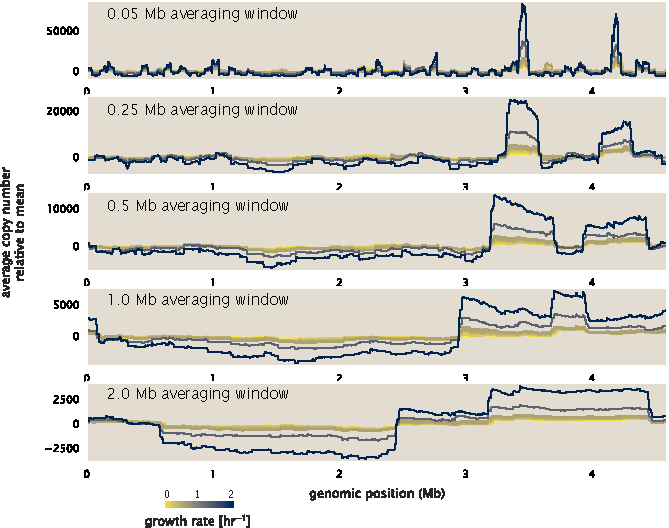
\includegraphics{SI_figs/supplemental_boxcar2.pdf} \caption{\textbf{Position-dependent protein expression at different growth rates.} (A) Protein copy number is reported along the length of the chromosome using a boxcar averaging. Here we consider different averaging window sizes:
% 0.05 Mb, 0.25 Mb, 0.5 Mb, 1.0 Mb, and 2 Mb. }
% \label{fig:supplemental_boxcar_2} }
% \end{fullwidth}
% \end{figure}


%
% \section{Hypothesis for increase in ribosomal abundance in the presence of chloramphenicol.}
%
% In the main text we note that the observed increase in ribosomal abundance  upon
% addition of non-lethal concentrations of chloramphenicol may in part  be a
% consequence of limiting rRNA production. Specifically, the proposal assumes that
% RNA polymerase are producing rRNA at their maximal rate (i.e. maximal packing of
% RNA polymerase on each rRNA operon). By sequestering ribosomes there will be a
% decrease in protein synthesis rate (i.e. lower $r_t \cdot R$) and a
% corresponding increase in doubling time. Qualitatively then, we may then expect
% that that more rRNA (and therefore more ribosomes) may be produced for a
% specific growth condition and longer doubling times  Figure
% \ref{fig:Si_Cm}(A).
%
% Here we consider data from Si \textit{et al.} (2017) where cells were grown in
% the presence of sub-lethal levels of chloramphenicol. In Figure \ref{fig:Si_Cm}(B) we
% plot measured RNA-to-protein ratios as a function of $\langle$\#ori$\rangle$ /
% $\langle$\# ter$\rangle$ (calculated using their reported values of $\tau_C$ and
% $\tau$). While the data is relatively noisy, we do see that
% increasing concentrations of chloramphenicol is associated with an increased
% RNA-to-protein ratios and this appears roughly independent of the particular
% $\langle$\#ori$\rangle$ / $\langle$\# ter$\rangle$ ratio.
%
% One challenge in interpreting the data is that the $\langle$\#ori$\rangle$ /
% $\langle$\# ter$\rangle$ ratio for a specific growth condition tends to decrease
% with increasing concentrations of chloramphenicol (indicated by marker type).
% Since the $\langle$\#ori$\rangle$ / $\langle$\# ter$\rangle$ ratio is defined by
% the ratio $\tau_C$/ $\tau$, this is likely a reflection of chloramphenicol
% slowing down protein production relative to the rate of DNA replication (though,
% both $\tau_C$ and $\tau$ increase with added chloramphenicol).
%
% Lastly, using the reported cell size data that was also available, we also
% consider how total ribosome copy number varies with growth condition and
% chloramphenicol. Here, as a first approaximation we assume that the total
% protein per cell will is proportional to cell size (with total protein $\approx$
% cell volume x 1.1 g/ml x 30\% dry mass x 55\% protein). We then estimate the
% number of ribosomes by multiplying the protein mass by our estimate of the
% ribosomal fraction.  Consistent with the apparent generality in how growth
% relates to cell size (size $\propto$ $\langle$\#ori$\rangle$) \citep{si2017},
% the number of ribosomes per cell collapse  onto a roughly linear trend with
% respect to the  $\langle$\#ori$\rangle$ (Figure \ref{fig:Si_Cm}(C)).
%
% That each of the chloramphenicol curves do not collapse onto a single line when
% normalized relative to $\langle$\#ori$\rangle$ (Figure \ref{fig:Si_Cm}(D))
% may be a reflection of biosynthetic rates increasing overall in richer media.
% For protein translation specifically, the rate of translation increases in both
% nutrient-limitation \citep{scott2010}, and with increasing concentrations of
% chloramphenicol \citep{dai2016} for poorer media (up to maximum of about 17 aa
% per second). It may be that other processes, and production of rRNA in
% particular may also slow down in poorer media.
%
% \begin{figure}
%     \begin{fullwidth}
%         \centering{
% 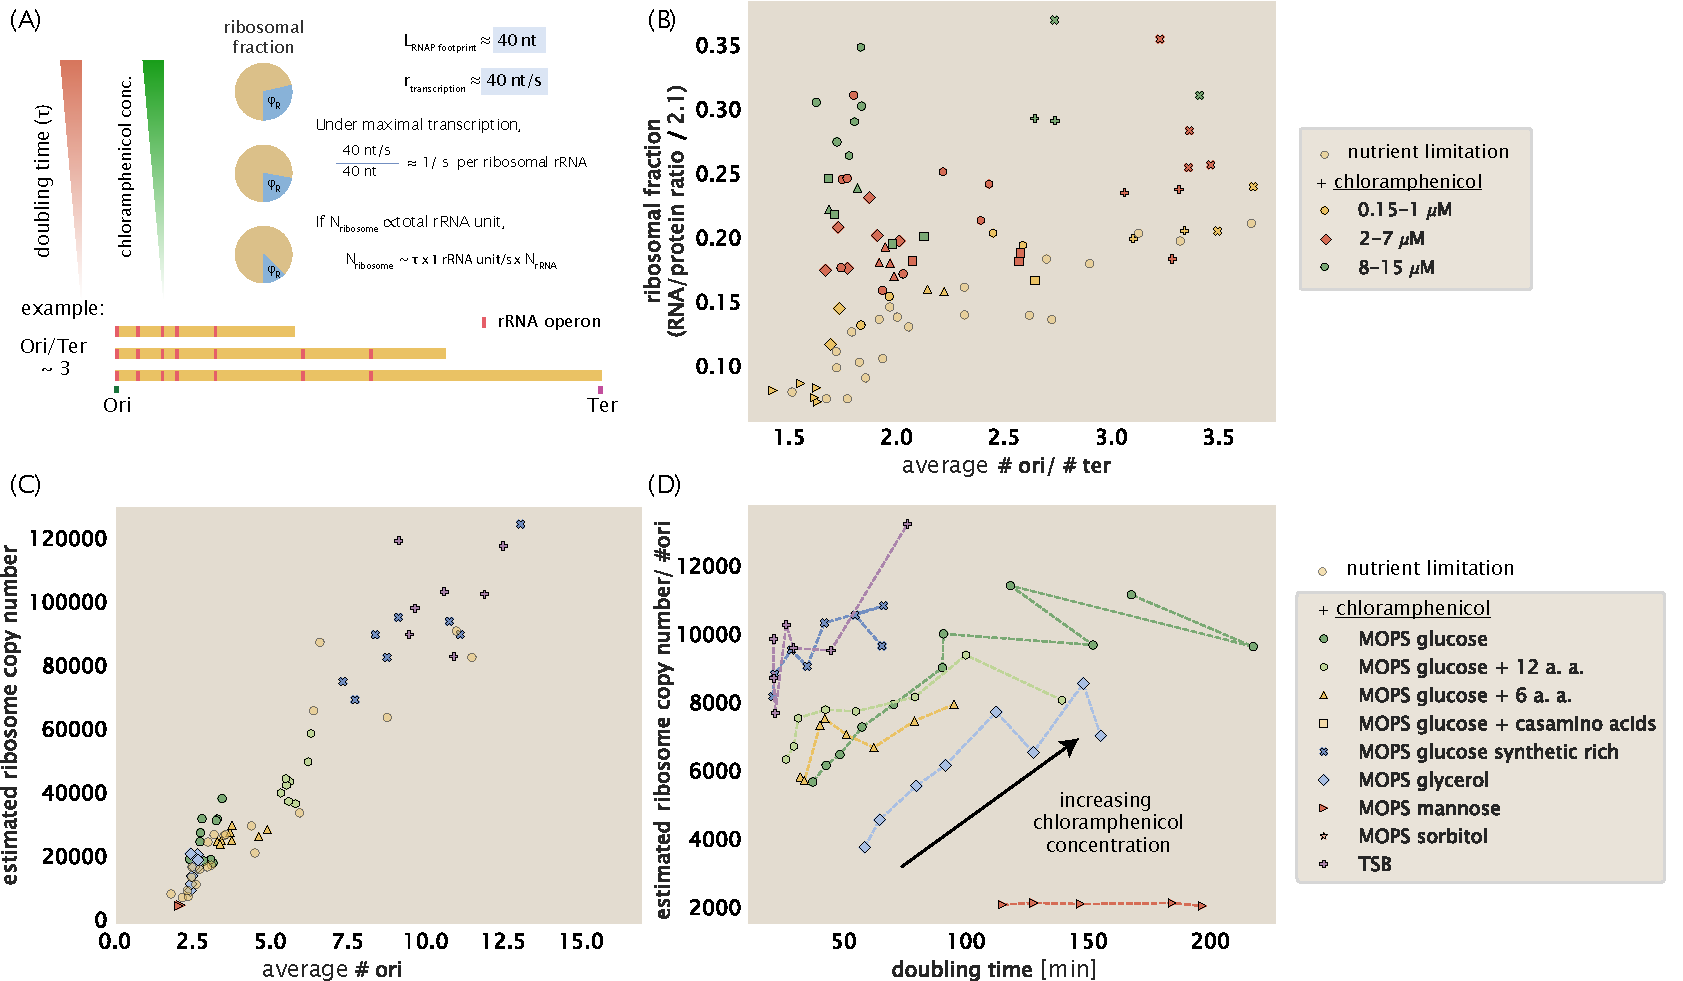
\includegraphics[width=1.2\textwidth]{SI_figs/supplemental_Si_Cm.pdf} \caption{\textbf{Potential effect of
%     chloramphenicol on ribosomal abundance of if rRNA production is limiting.}
%     (A) Schematic of proposed change in ribosomal abundance upon addition of non-lethal
%     does of chloramphenicol. We consider, for example, a $\langle$\#ori$\rangle$ / $\langle$\#ter$\rangle$ ratio of ~ 3, which reflects an effective chromosome whose gene dosage is biased more so to regions near the origin. If ribosome production is limited by
%     rRNA production in particular, then sequestering ribosomes will slow down
%     cell doubling and provide addition time for more rRNA to be made.
%     (B) Estimated ribosomal fraction ($\approx$ RNA/protein ratio x 2.1 \cite{dai2016}) at
%     as a function of measured $\langle$\#ori$\rangle$ / $\langle$\# ter$\rangle$ ratio. Data is
%     split into 'nutrient-limited' growth (pale yellow), low chloramphenicol concentration (yellow, 0.15 - 1 $\mu$M), medium chloramphenicol concentration (red, 2 - 7 $\mu$M), and
%     high chloramphenicol concentration (red, 8 - 15 $\mu$M). Marker type corresponds to
%     the growth media as indicated in part (C).
%     (C) Scaling of estimated ribosomal copy number with $\langle$\#ori$\rangle$, showing that
%     cells still scale their total protein in accord with apparent growth law \citep{si2017}
%     irrespective of presence of chloramphenicol.
%     (D) Estimated ribosomal copy number normalized by $\langle$\#ori$\rangle$. Data shows
%     a media-specific increase in ribosomal abundance per origin with longer doubling times.
%     All data is from \citep{si2017}, and show that average values from each growth condition and chloramphenicol concentration (including data from both strains, MG1655 and NCM3722).}
% \label{fig:Si_Cm} }
% \end{fullwidth}
% \end{figure}
%
%



\newpage
%%%%%%%%%%%%%%%%%%%%%%%%%%%%%%%%%%%%%%%%%%%%%%%%%%%%%%%%%%%%
%%% Bib START
%%%%%%%%%%%%%%%%%%%%%%%%%%%%%%%%%%%%%%%%%%%%%%%%%%%%%%%%%%%%
\bibliography{library.bib}

\end{document}
